\documentclass{nwureport}
\RequirePackage[l2tabu, orthodox]{nag}
\ifx\pdftexversion\undefined
\usepackage[dvips]{graphicx}
\else
\usepackage[pdftex]{graphicx}
% Only print picture outlines...
%\usepackage[pdftex,draft]{graphicx}
\DeclareGraphicsRule{*}{mps}{*}{}
\fi

\usepackage{caption}
\usepackage{siunitx}
\usepackage{hyperref}

\usepackage{minitoc}
\usepackage{pdfpages}
\usepackage{dirtree}
\usepackage[toc,page]{appendix}
%\usepackage[a4paper,lmargin=3.0cm, rmargin=1.0cm,tmargin=3.5cm,bmargin=2.50cm]{geometry}

%%%%%%%%%%%%%%%%%%%%%%%%%%%%%%%%%%%%%%%%%%%%%%%%%%%%%%%
% Reset text/figure fractions to more reasonable values
%%%%%%%%%%%%%%%%%%%%%%%%%%%%%%%%%%%%%%%%%%%%%%%%%%%%%%%
\renewcommand{\topfraction}{0.85}
\renewcommand{\textfraction}{0.1}
\renewcommand{\floatpagefraction}{0.79}
%%%%%%%%%%%%%%%%%%%%%%%%%%%%%%%%%%%%%%%%%%%%%%%%%%%%%%%
% Working
%\renewcommand{\topfraction}{0.85}
%\renewcommand{\textfraction}{0.}
%\renewcommand{\floatpagefraction}{0.79}
%%%%%%%%%%%%%%%%%%%%%%%%%%%%%%%%%%%%%%%%%%%%%%%%%%%%%%%

\graphicspath{{./images/}}

\usepackage{longtable}
%\usepackage{fullpage} % reduce margin whitespace
%\usepackage{setspace} % 

% This makes TOC and lists have very little white spacing...
\usepackage{tocloft}
%%%%%%%%%%%%%%%%%%%%%%%%%%%%%%%%%%%%%%%%%%%%%%%%%%%%%%%
% Draft assistance
%%%%%%%%%%%%%%%%%%%%%%%%%%%%%%%%%%%%%%%%%%%%%%%%%%%%%%%
%\usepackage{showkeys}
%\usepackage{showlabels}
%\usepackage{everypage}
%\usepackage{draftwatermark}
%%%%%%%%%%%%%%%%%%%%%%%%%%%%%%%%%%%%%%%%%%%%%%%%%%%%%%%

\usepackage{times} % font

\usepackage{booktabs}

\usepackage{multirow}

\usepackage{cmap}     % to produce searchable PDF

\usepackage{rotating,lscape}

%%%%%%%%%%%%%%%%%%%%%%%%%%%%%%%%%%%%%%%%%%%%%%%%%%%%%%%
% Page style - footers and headers
%%%%%%%%%%%%%%%%%%%%%%%%%%%%%%%%%%%%%%%%%%%%%%%%%%%%%%%
\usepackage{fancyhdr}
\usepackage{tocloft}
\pagestyle{fancy}

\renewcommand{\chaptermark}[1]{\markboth{\thechapter.\ #1}{}} 
\fancyhead{} % clear all header fields

\fancypagestyle{plain}{%
  \renewcommand{\headrulewidth}{0pt}% Header rule thickness
  \renewcommand{\footrulewidth}{0pt}% Footer rule thickness
  \fancyhf{}% Clear header/footer
  \fancyhead[L]{}% Chapter in header Left
  \renewcommand{\headrulewidth}{\iffloatpage{0pt}{0pt}}
  \fancyfoot[C]{-\thepage-} % Page number at the bottom 
}
%\fancypagestyle{frontmatter}{%
%  \renewcommand{\headrulewidth}{0pt}% No header rule
%  \renewcommand{\footrulewidth}{0pt}% No footer rule
%  \fancyhf{}% Clear header/footer
%  \fancyfoot[C]{-\thepage-}%
%}
\fancypagestyle{mainmatter}{%
  \renewcommand{\headrulewidth}{0pt}% Header rule
  \renewcommand{\footrulewidth}{0pt}% Footer rule
  \fancyhf{}% Clear header/footer
%  \fancyhead[L]{\scshape\leftmark}% Chapter in header Left
  \fancyhead[R]{Assessing the source contribution to atmospheric particulate matter in Wedela}% Page number in header Right
  \renewcommand{\headrulewidth}{\iffloatpage{0pt}{0pt}}
  \fancyfoot[C]{-\thepage-} % Page number at the bottom 
}

%doesn't work
%%\addtolength{\headheight}{5pt} 
%%\cfoot[]{-\thepage-}
%\fancyfoot{} % clear all footer fields
%\fancyfoot[C]{-\thepage-}
%%\renewcommand{\headrulewidth}{0pt}
%%\renewcommand{\footrulewidth}{0pt}

%%%%%%%%%%%%%%%%%%%%%%%%%%%%%%%%%%%%%%%%%%%%%%%%%%%%%%%

\usepackage[section]{placeins}

\usepackage{amsmath,url}
\usepackage{subeqnarray}

%pdfpagelabels, % Need to solve the figure count reset to use this
%%%%%%%%%%%%%%%%%%%%%%%%%%%%%%%%%%%%%%%%%%%%%%%%%%%%%%%%%%%%%
% Hyperref pdf options
%%%%%%%%%%%%%%%%%%%%%%%%%%%%%%%%%%%%%%%%%%%%%%%%%%%%%%%%%%%%%
\usepackage[pdftitle={Assessing the source contribution to atmospheric particulate matter in Wedela},pdfpagemode=UseOutlines,colorlinks,pdfauthor={Roelof
    Burger},bookmarks=true,pdftex=true,hyperindex,plainpages=false,pdfpagelabels,pagebackref]{hyperref}
%\hypersetup{colorlinks,linkcolor=black,citecolor=black,pdfstartview=Fit}
\hypersetup{pdfstartview=Fit}
%%%%%%%%%%%%%%%%%%%%%%%%%%%%%%%%%%%%%%%%%%%%%%%%%%%%%%%%%%%%%

%%%%%%%%%%%%%%%%%%%%%%%%%%%%%%%%%%%%%%%%%%%%%%%%%%%%%%%%%%%%%
% TOC font settings
%%%%%%%%%%%%%%%%%%%%%%%%%%%%%%%%%%%%%%%%%%%%%%%%%%%%%%%%%%%%%
%\usepackage[titles]{tocloft}
%\renewcommand{\cfttoctitlefont}{\sffamily}
%%%%%%%%%%%%%%%%%%%%%%%%%%%%%%%%%%%%%%%%%%%%%%%%%%%%%%%%%%%%%
% Advanced glossaries package
%%%%%%%%%%%%%%%%%%%%%%%%%%%%%%%%%%%%%%%%%%%%%%%%%%%%%%%%%%%%%
\usepackage[toc,style=long]{glossaries}
%%%%%%%%%%%%%%%%%%%%%%%%%%%%%%%%%%%%%%%%%%%%%%%%%%%%%%%%%%%%%

\usepackage{enumerate}
\usepackage{verbatim}  %  This is to use \begin{comment} ...

%\usepackage{sectsty}
%\allsectionsfont{\usefont{OT1}{phv}{bc}{n}\selectfont}
%\usepackage[sf]{titlesec}


%%%%%%%%%%%%%%%%%%%%%%%%%%%%%%%%%%%%%%%%%%%%%%%%%%%%%%%%%%%%%
% Glossaries and abbreviations
%%%%%%%%%%%%%%%%%%%%%%%%%%%%%%%%%%%%%%%%%%%%%%%%%%%%%%%%%%%%%
\usepackage[toc,style=long]{glossaries}

\newglossary{abbreviation}{aot}{ata}{Abbreviations}
%\newglossary{compounds}{cot}{cts}{List of Compounds}
% \newglossary{symbols}{sot}{sts}{List of Symbols}
\loadglsentries[abbreviation]{abbreviations}
%\loadglsentries[compounds]{compounds}
% \loadglsentries[symbols]{symbols}
\makeglossaries
%%%%%%%%%%%%%%%%%%%%%%%%%%%%%%%%%%%%%%%%%%%%%%%%%%%%%%%%%%%%%

\usepackage{natbib}
\begin{document}
\bibliographystyle{crg}

     \title{Asessing the source contribution to atmospheric particulate matter in Wedela}
     %\title{The establishment of rain gauge networks for rainfall estimation calibration of the South African new weather network}
     \author{
        Roelof Burger
          \thanks{
             Climatology Research Group\\
             Unit for Environmental Sciences and Management \\
             North-West University, Potchefstroom, 2520, South Africa \\
             {\tt roelof.burger@nwu.ac.za}} \\
     }
     \activity{Progress report}
     \projnumber{WEDANG01-QR1v1}
     \lab{Environmental Sciences and Management}
     \keywords{air quality, low-income settlements, townships, winter}
     \maketitle

\pagenumbering{roman}

\chapter*{Executive Summary}

\pagebreak

\chapter*{Acknowledgments}

The data was collected by:
\\
\begin{tabular}{ l l } 
Joe Malahlela  & NWU \\
Thomas Bigala  & NWU \\
Roelof Burger  & NWU \\
Marvin Qhekwana & NWU \\
Thapelo Letsolo & NWU \\
\end{tabular}

\clearpage

\dominitoc
\setcounter{tocdepth}{2} % set depth level of TOC
\pagestyle{plain}
{\thispagestyle{plain}
\tableofcontents
% Add page heading 
\addtocontents{toc}{~\hfill\textbf{Page}\par}
\addcontentsline{toc}{chapter}{Contents}
\clearpage
\listoffigures
\addtocontents{lof}{~\hfill\textbf{Page}\par}
\addcontentsline{toc}{chapter}{Figures}
\clearpage
\listoftables
\addtocontents{lot}{~\hfill\textbf{Page}\par}
\addcontentsline{toc}{chapter}{Tables}
%\clearpage
\printglossaries
%\clearpage
}

\pagenumbering{arabic}
\pagestyle{mainmatter}

%%%%%%%%%%%%%%%%%%%%%%%%%%%%%%%%%%%%%%%%%%%%%%%%%%%%%%%%%%%%%

\chapter{Introduction}

This report describes the 

%\minitoc

%%%%%%%%%%%%%%%%%%%%%%%%%%%%%%%%%%%%%%%%%%%%%%%%%%%%%%%%%%%%%

\chapter{Proposed methodology}

\section{Site description}
Wedela is a small, low income settlement located in the Gauteng province of
South-Africa (26°27'58"S 27°23'0"E). The settlement is in close proximity to Carltonville
and also less than 80km from Johannesburg, the area is also known for the various goldmines
that operate in the area. \hyperref[fig:wadela]{Figure \ref{fig:wadela}}
indicates the relative position of Wedela in South-Africa and in proximity to other major
in the region.

\begin{figure}[!htb]
    \centering
    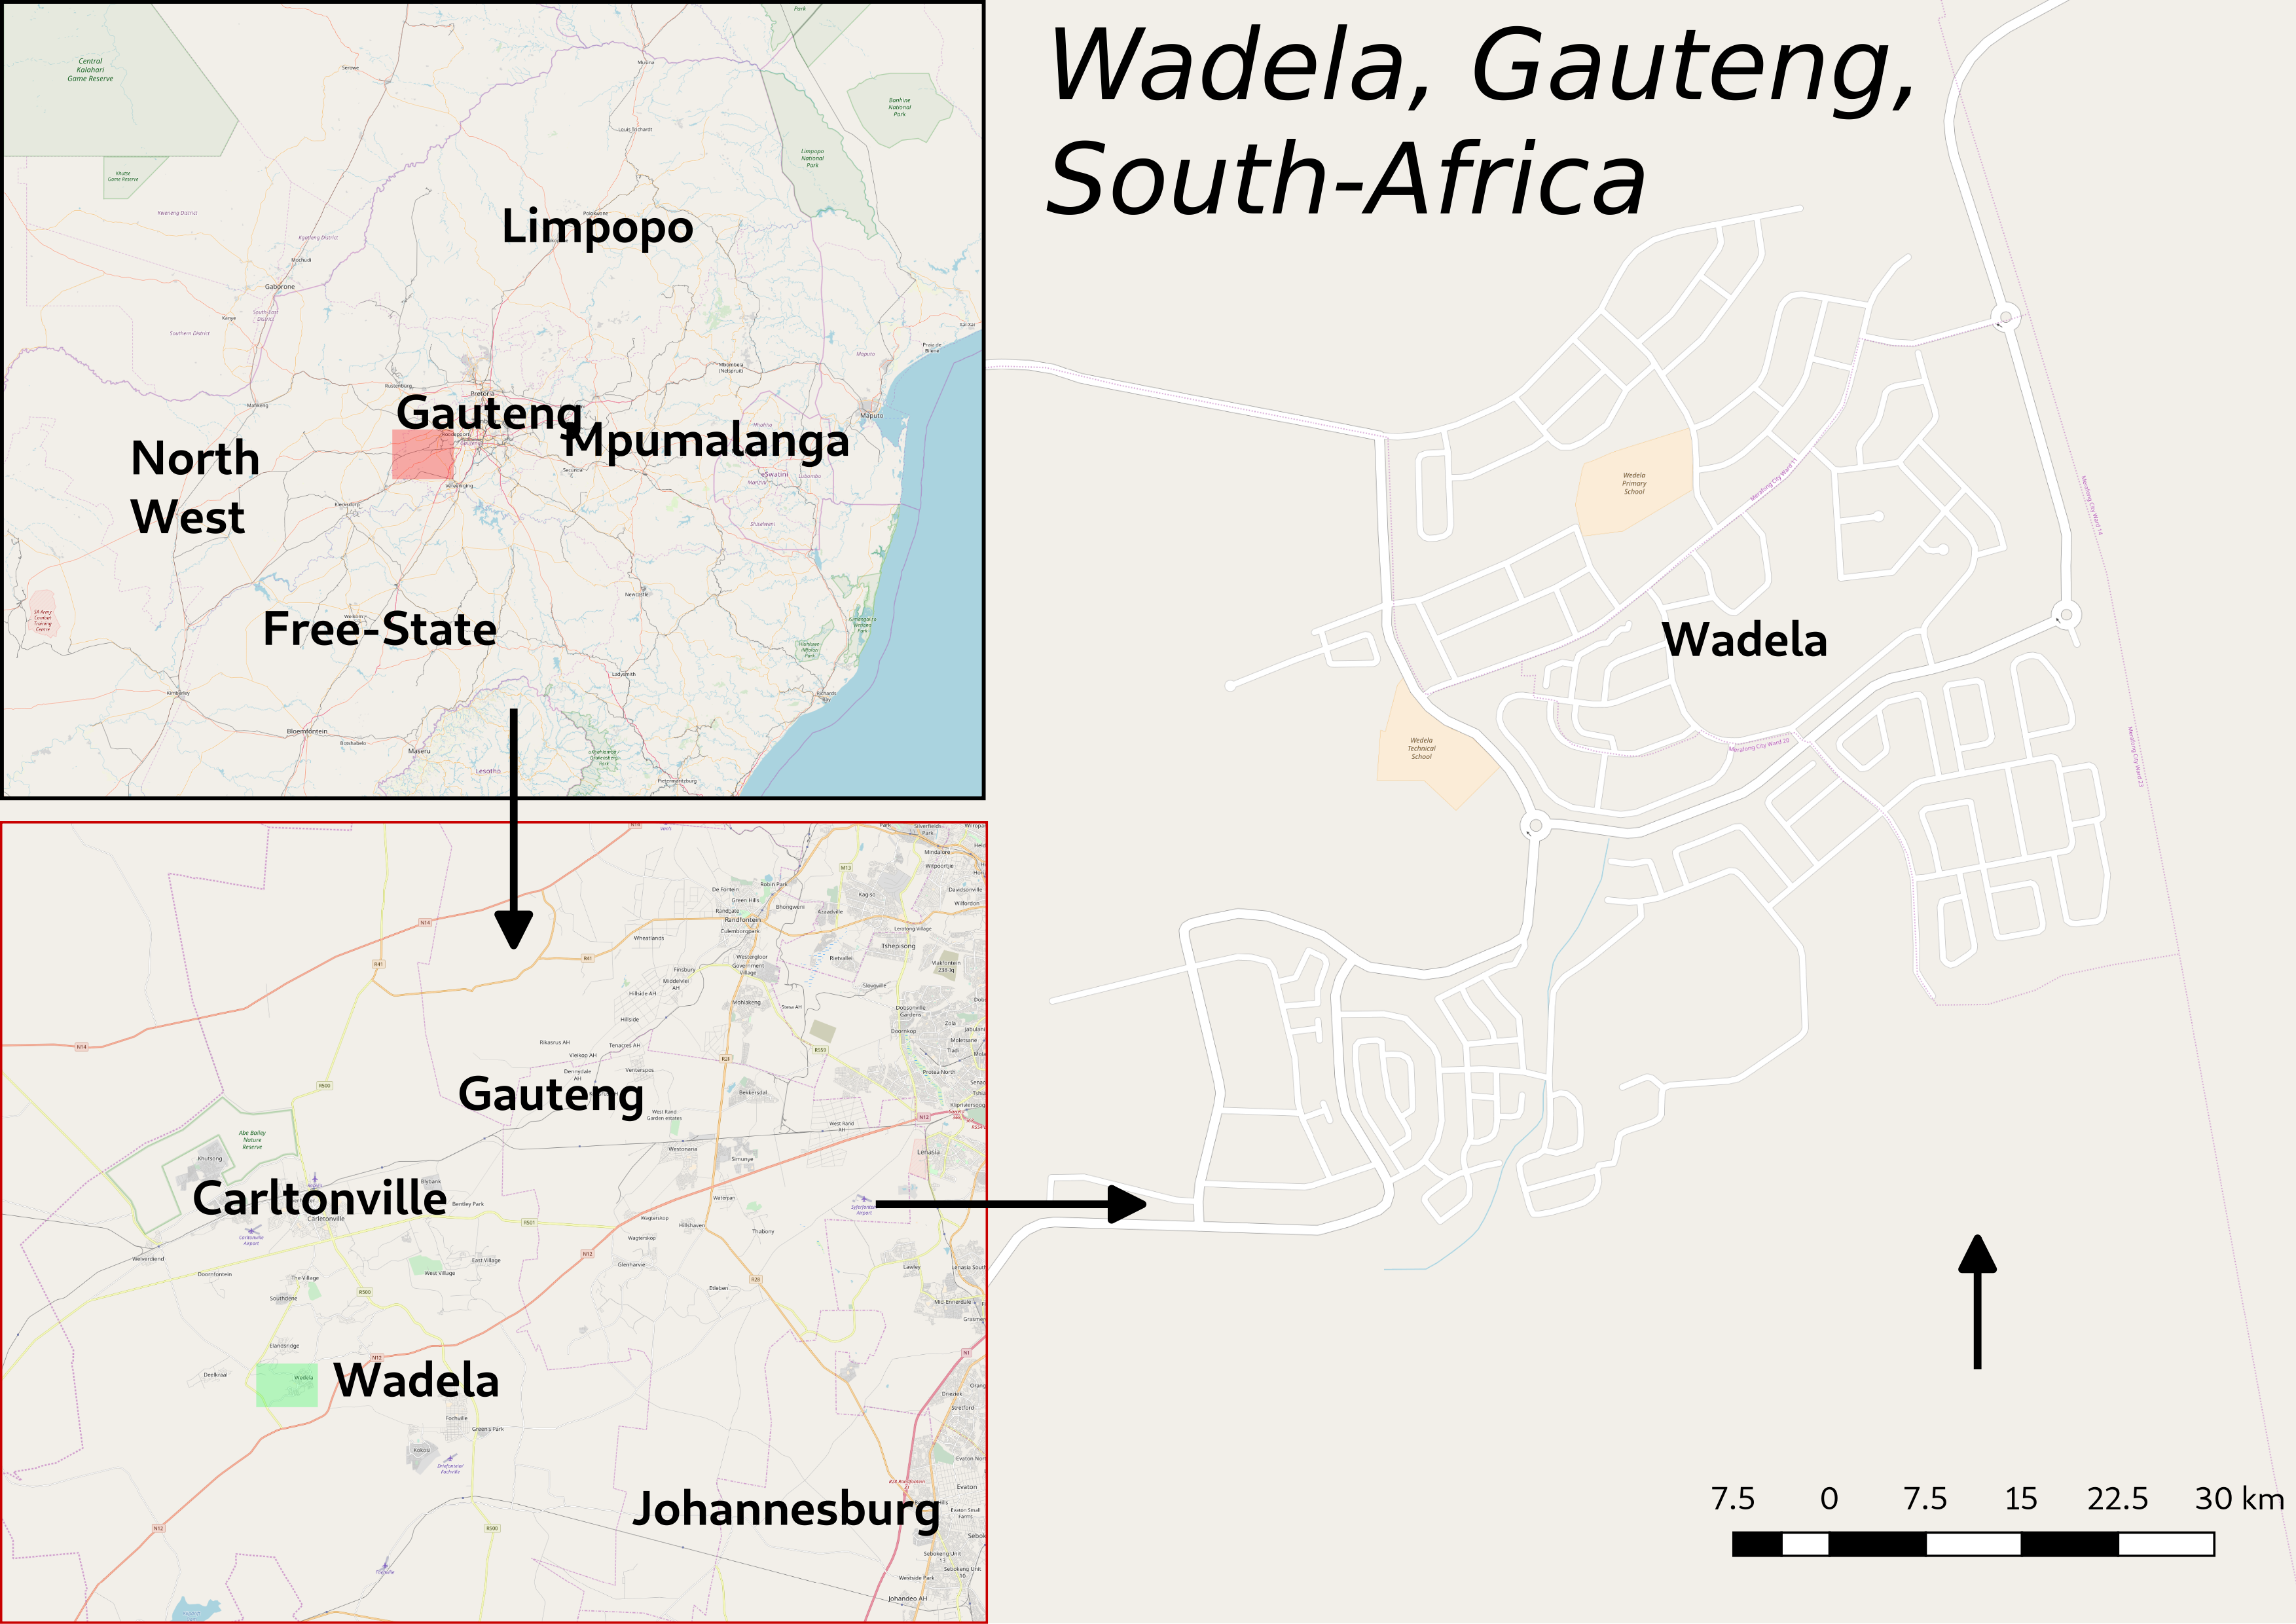
\includegraphics[width=\textwidth]{images/study_area_qgis.png}
    \caption[Study area: Wedela, Gauteng]{Wedela, seen in the above map, is the location where
    the study was conducted. The settlement is located in close proximity to Carltonville and Johannesburg.
    There is also various gold mines present in the region. The map shows Wedela's relative position in
    South-Africa as indicated in the overlay maps.}
    \label{fig:wadela}
\end{figure}


\section{Characterizing ambient particulate matter}
Two EBAMs, one PM10 and one PM2.5 

Talk to Lucky, survey, source profiles

\subsection{Instruments}


\begin{figure}[!htb]
    \centering
    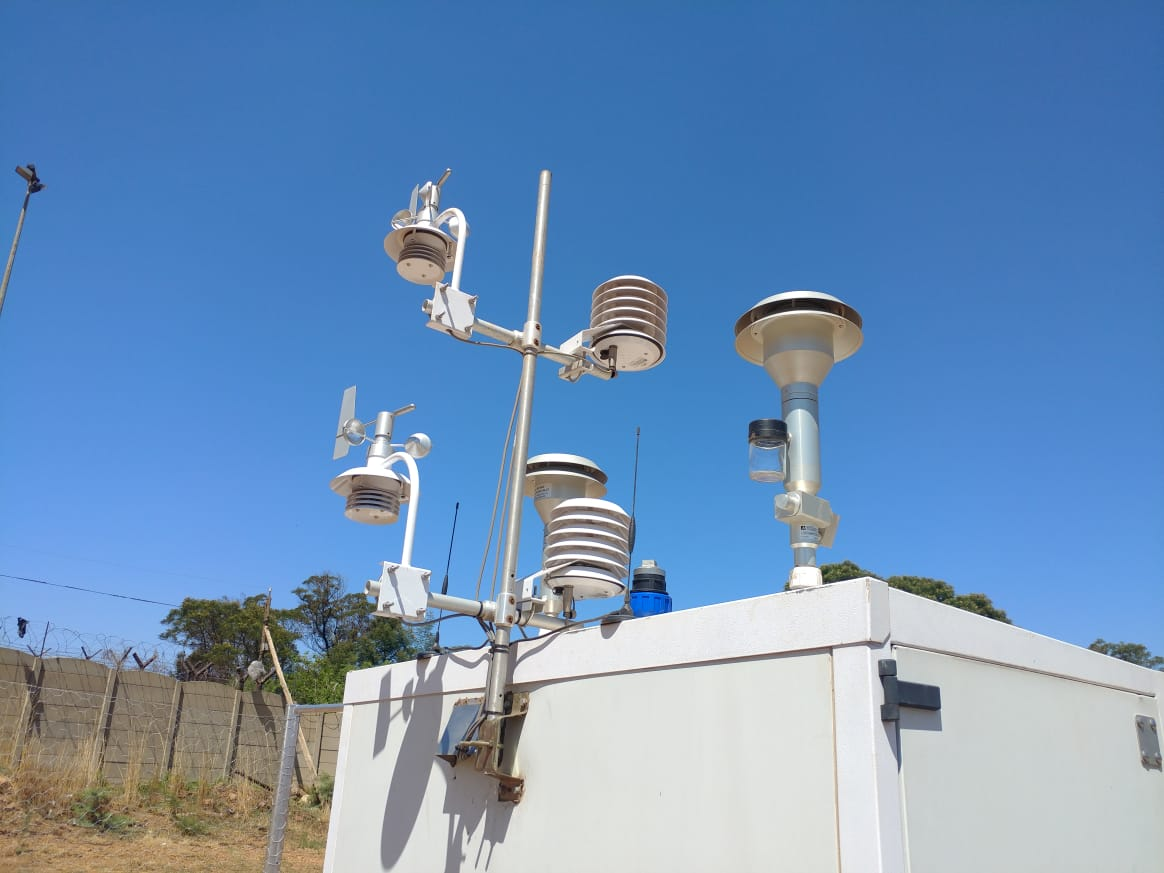
\includegraphics[width=\textwidth]{images/wedela.jpeg}
    \caption[]{Caption}
    \label{fig:wadela_instruments_met}
\end{figure}

\begin{figure}[!htb]
    \centering
    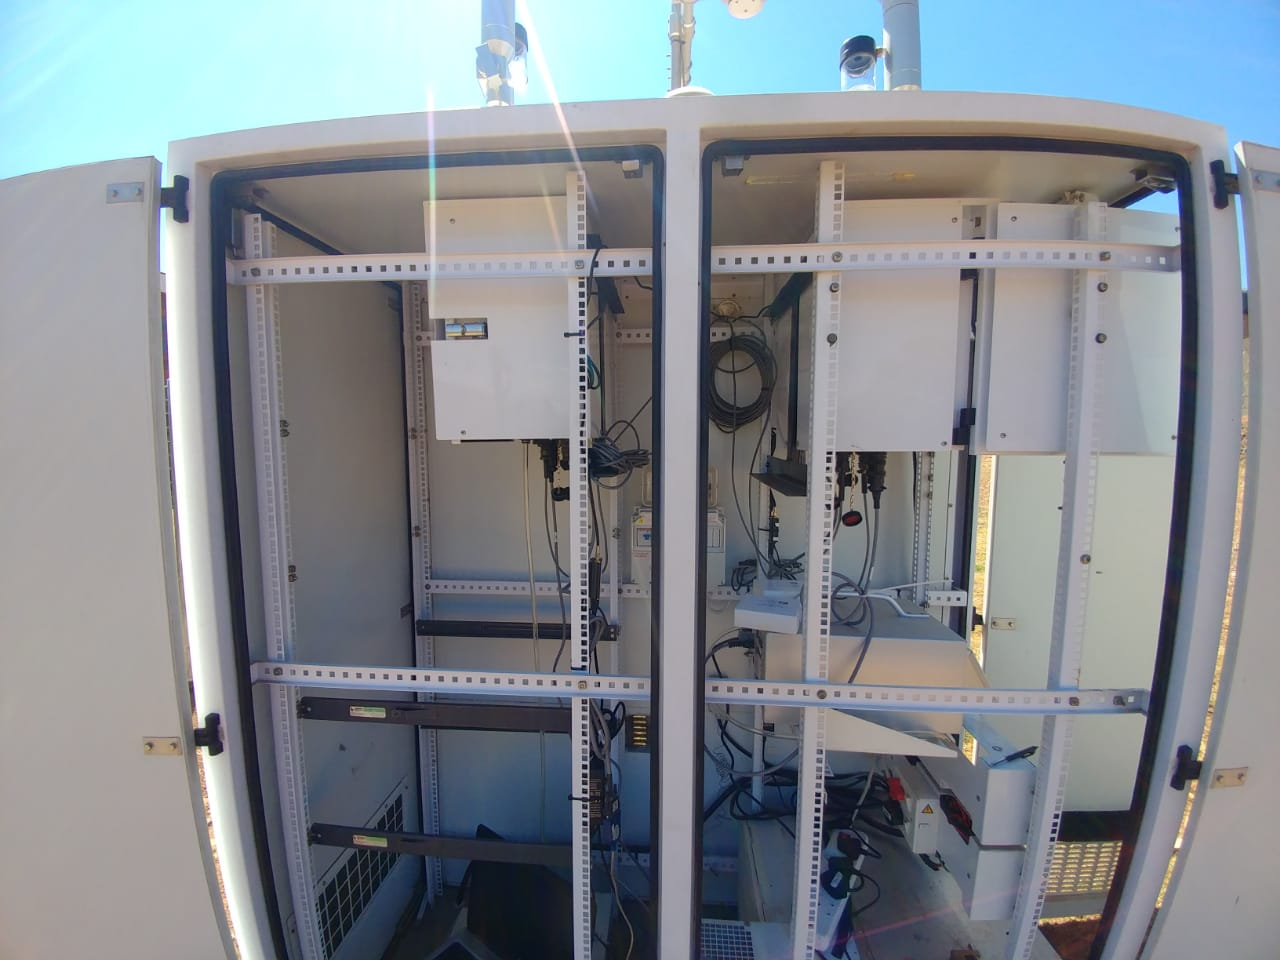
\includegraphics[width=\textwidth]{images/wadela_10.jpeg}
    \caption[]{Caption}
    \label{fig:wadela_instruments_pm}
\end{figure}

\begin{figure}[!htb]
    \centering
    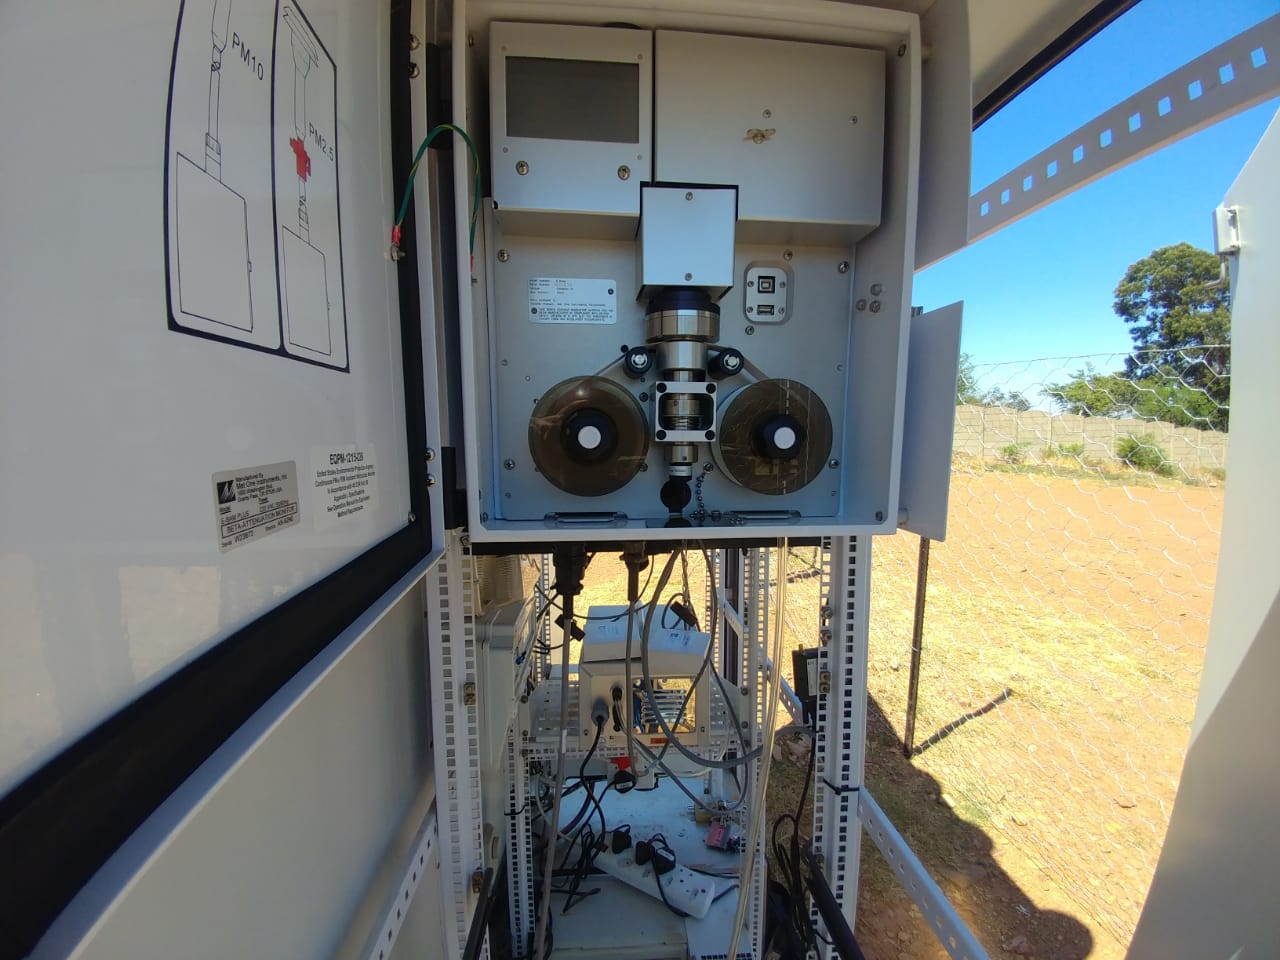
\includegraphics[width=\textwidth]{images/wedela_6.jpeg}
    \caption[]{Caption}
    \label{fig:wadela_instruments_pm2}
\end{figure}

\section{Characterizing sources of particulate matter}

\section{Characterizing sources contribution}

Source apportionment methodology

\section{Modelling ambient concentrations}

Dispersion modelling using AERMOD

\section{Realtime data access}

A real-time monitoring solution has been established through \url{www.ecostat.co.za} to
the EBAM PM2.5 and PM10 instruments located in Wadela. Ecostat allows users to access the data
through any browser such as Firefox, Chrome or Internet Explorer. 

Ecostat has various functions to enable data monitoring in real-time, this includes
viewing the status of the data logging as seen in \hyperref[fig:ecostat_status]{figure \ref{fig:ecostat_status}}. The status reports assists the project technical staff to avoid
unnecessary travel while researchers can access the raw data to do quality control checks. 

\begin{figure}[!htb]
    \centering
    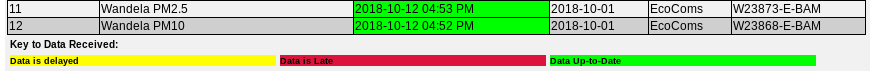
\includegraphics[width=\textwidth]{images/ecstat_status.png}
    \caption[Ecostat.co.za status report]{Caption}
    \label{fig:ecostat_status}
\end{figure}

Ecostat further allows quick view products of the instrument status,
meteorological and pollution data from the site location as seen
in \hyperref[fig:ecostat_quick]{figure \ref{fig:ecostat_quick}}. This is
valuable to quickly asses current ambient environment and also to check the
instrument for unrealistic or erroneous values.

\begin{figure}[!htb]
    \centering
    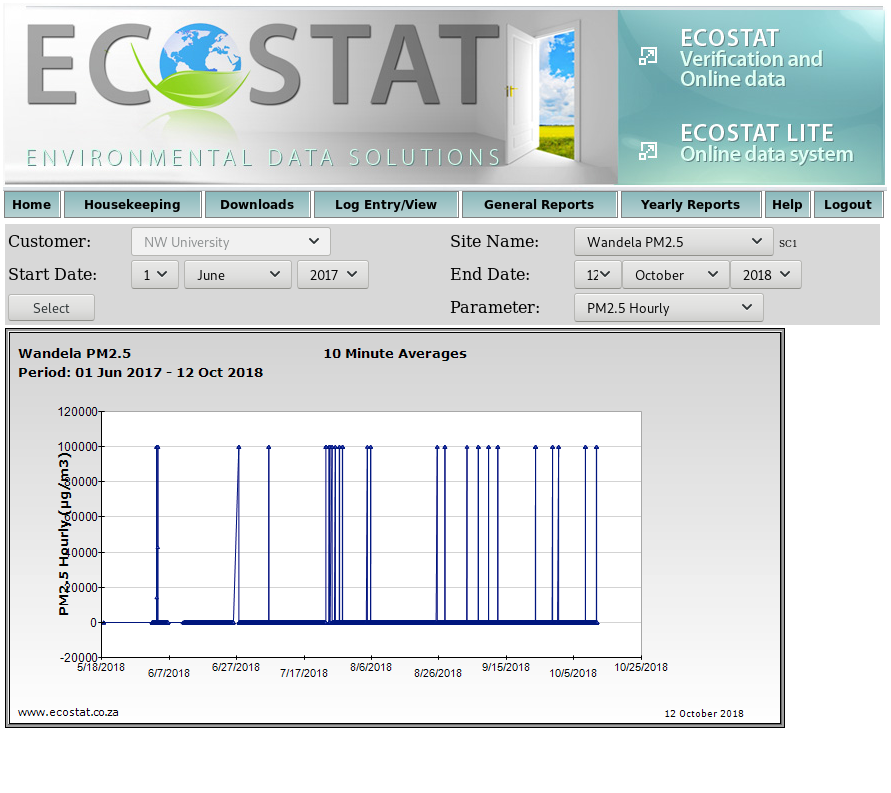
\includegraphics[width=\textwidth]{images/ecostat_quick.png}
    \caption[Ecostat.co.za quick view]{Caption}
    \label{fig:ecostat_quick}
\end{figure}

%%%%%%%%%%%%%%%%%%%%%%%%%%%%%%%%%%%%%%%%%%%%%%%%%%%%%%%%%%%%%

\chapter{Site preparation and installation}

\section{Identifying potential sites}

\section{Electricity supply for the instrument}

\section{Security and access control}
All instruments are located within a fenced perimeter in Wadela. Only technicians and
research staff have access to the site.

\begin{figure}[!htb]
    \centering
    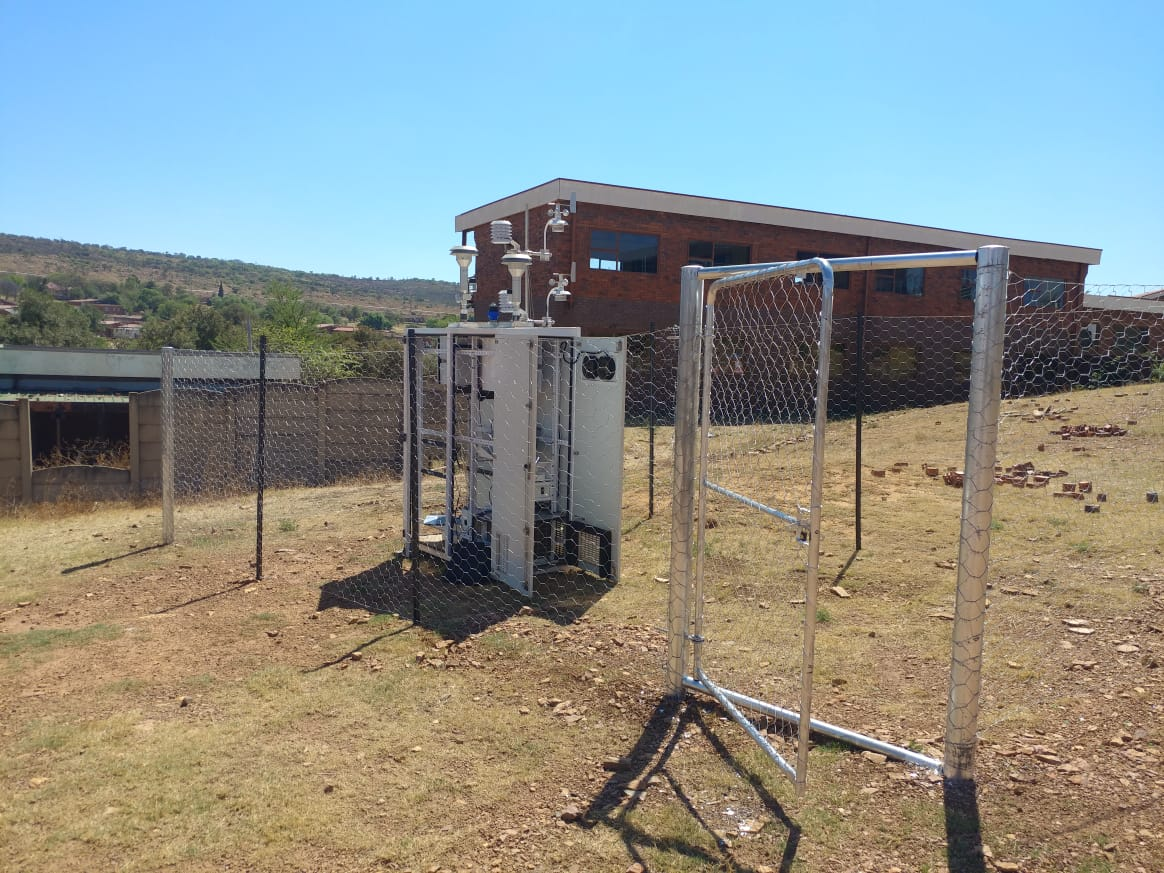
\includegraphics[width=\textwidth]{images/wedela_4.jpeg}
    \caption[Security and access control at the Wedela measuring site]{Security and access control at the Wedela measuring site}
    \label{fig:wadela_fence}
\end{figure}

\section{Community engagement}

%%%%%%%%%%%%%%%%%%%%%%%%%%%%%%%%%%%%%%%%%%%%%%%%%%%%%%%%%%%%%

\chapter{Measurements of atmospheric particulate matter}

\section{File conventions}

All final datasets are stored in \gls{ascii} format with extensions
``.txt'' and ``.csv''. This is the most
widely accepted format readable by most software. The most common
convention is simple \gls{csv}, usually denoted with the extension
``.csv''. Most of the data acquisition devices
store data in \gls{ascii}, these raw files are kept untouched. All
binary formats are converted into \gls{csv} files. Staring all
data-sets in \gls{ascii} will ensure that all users will have easy
access to the data and any future changes to commercial software will
not impact on its accessibility.

Excel is the most common software used for data processing. \gls{csv}
files easily integrates with most import and export facilities of
Excel. Special care must be taken when using the following features:

\begin{description}
\item [Importing files] A field separator should be chosen when
  importing files into Excel. The default separator is a comma
  (,). This implies that a comma should not be used anywhere in data
  files other than for denoting a field separator. It is very likely
  that commas will be present if there are long strings or written
  descriptions in a file. In these cases, a pipe (\textbar) can be used as a
  separator. These instances should be avoided as far as possible.
\item [Formatting of cells] Care must be exercised when processing or
  formatting data in excel. The formatting of each cell in Excel
  depends on the settings. It frequently looks different from the raw
  data. If the user are not aware of the current formatting setting of
  the cell, row or column, mistakes will be made when importing or
  exporting data. The most common places for these mistakes comes when
  dealing with dates, times, percentages and decimal characters.
\item [Exporting files] Final data-sets is stored in \gls{csv}. This is
  a standard export feature of Excel. The following features of most
  current versions of Excel must be taken into consideration when
  exporting files to \gls{csv}. If the Excel files contains many
  sheets, only the active sheet will be saved to \gls{csv} per export
  action. Each sheet must therefore be saved to a separate file.
\item [Using inverted commas (``)] Inverted commas typically has a
  special meaning in Excel. It is used to denote a text string for
  that particular field. When encapsulating data points in inverted
  commas, the user invariable forces Excel to see that field as a text
  string. This will be problematic if the user wishes to use that
  field in any operations, like algebraic conversion or time series
  operations. For this reason, inverted commas should only be used to
  denote text strings. An example would be to prevent excel from splitting a
  long text description containing commas into fields when importing a
  \gls{csv} files with a comma as a separator.
\end{description}

\subsubsection{General procedure for data quality control}
The raw data-sets collected are merged and processed into a final data
set for analysis through the following steps:

\begin{enumerate}
\item Apply date and time corrections to each of the raw data files
  using the instrument logs
\item Merge each of the data-sets above into one uniform data-set
\item Apply masks to each instrument according to the instrument log
\item Perform automated quality control on each variable and flag problematic values
  \begin{itemize}
   \item Test for sensible observation date and time values.
   \item Flag data close to or below the instrument detection limit. 
   \item Flag data close to or above the instrument's maximum detectable limited
   \item Test the gradient of each instrument against realistic response times
   \item Test for spikes by comparing with values before and after
   \item Test for stuck values and set missing
   \item Flag climatological outliers
   \item Flag outliers using the median absolute deviation
  \end{itemize}
\item Each variable with its associated flags identified in the automated quality control is then reviewed manually by viewing time series plots. Each flag is carefully inspected and values are deemed real or set to missing if a problem is suspected.
\item Values close to or below the detection limit are finally set to the minimum detection limit of the particular instrument \citep{Croghan2003}.
\end{enumerate}

The general philosophy in quality assuring data is to aggressively
ignore data that are suspected to be from a faulty instrument. Extra
care is taken when dealing with extreme values and outliers. These are
not set to missing unless they are part of a time period where the
instrument did not appear to be operating optimally.
\subsubsection{General procedure for data quality control}
The raw data-sets collected are merged and processed into a final data
set for analysis through the following steps:

\begin{enumerate}
\item Apply date and time corrections to each of the raw data files
  using the instrument logs
\item Merge each of the data-sets above into one uniform data-set
\item Apply masks to each instrument according to the instrument log
\item Perform automated quality control on each variable and flag problematic values
  \begin{itemize}
   \item Test for sensible observation date and time values.
   \item Flag data close to or below the instrument detection limit. 
   \item Flag data close to or above the instrument's maximum detectable limited
   \item Test the gradient of each instrument against realistic response times
   \item Test for spikes by comparing with values before and after
   \item Test for stuck values and set missing
   \item Flag climatological outliers
   \item Flag outliers using the median absolute deviation
  \end{itemize}
\item Each variable with its associated flags identified in the automated quality control is then reviewed manualy by viewing time series plots. Each flag is carefully inspected and values are deemed real or set to missing if a problem is suspected.
\item Values close to or below the detection limit are finally set to the minimum detection limit of the particular instrument \citep{Croghan2003}.
\end{enumerate}

The general philosophy in quality assuring data is to aggressively
ignore data that are suspected to be from a faulty instrument. Extra
care is taken when dealing with extreme values and outliers. These are
not set to missing unless they are part of a time period where the
instrument did not appear to be operating optimally.

\section{Preliminary results}

The following section shows some of the results from the Wedela monitoring site that include meteorological
and pollution data (PM2.5 and PM10). A basic QC was applied to this data-set where missing values was removed.

\begin{figure}[!htb]
    \centering
    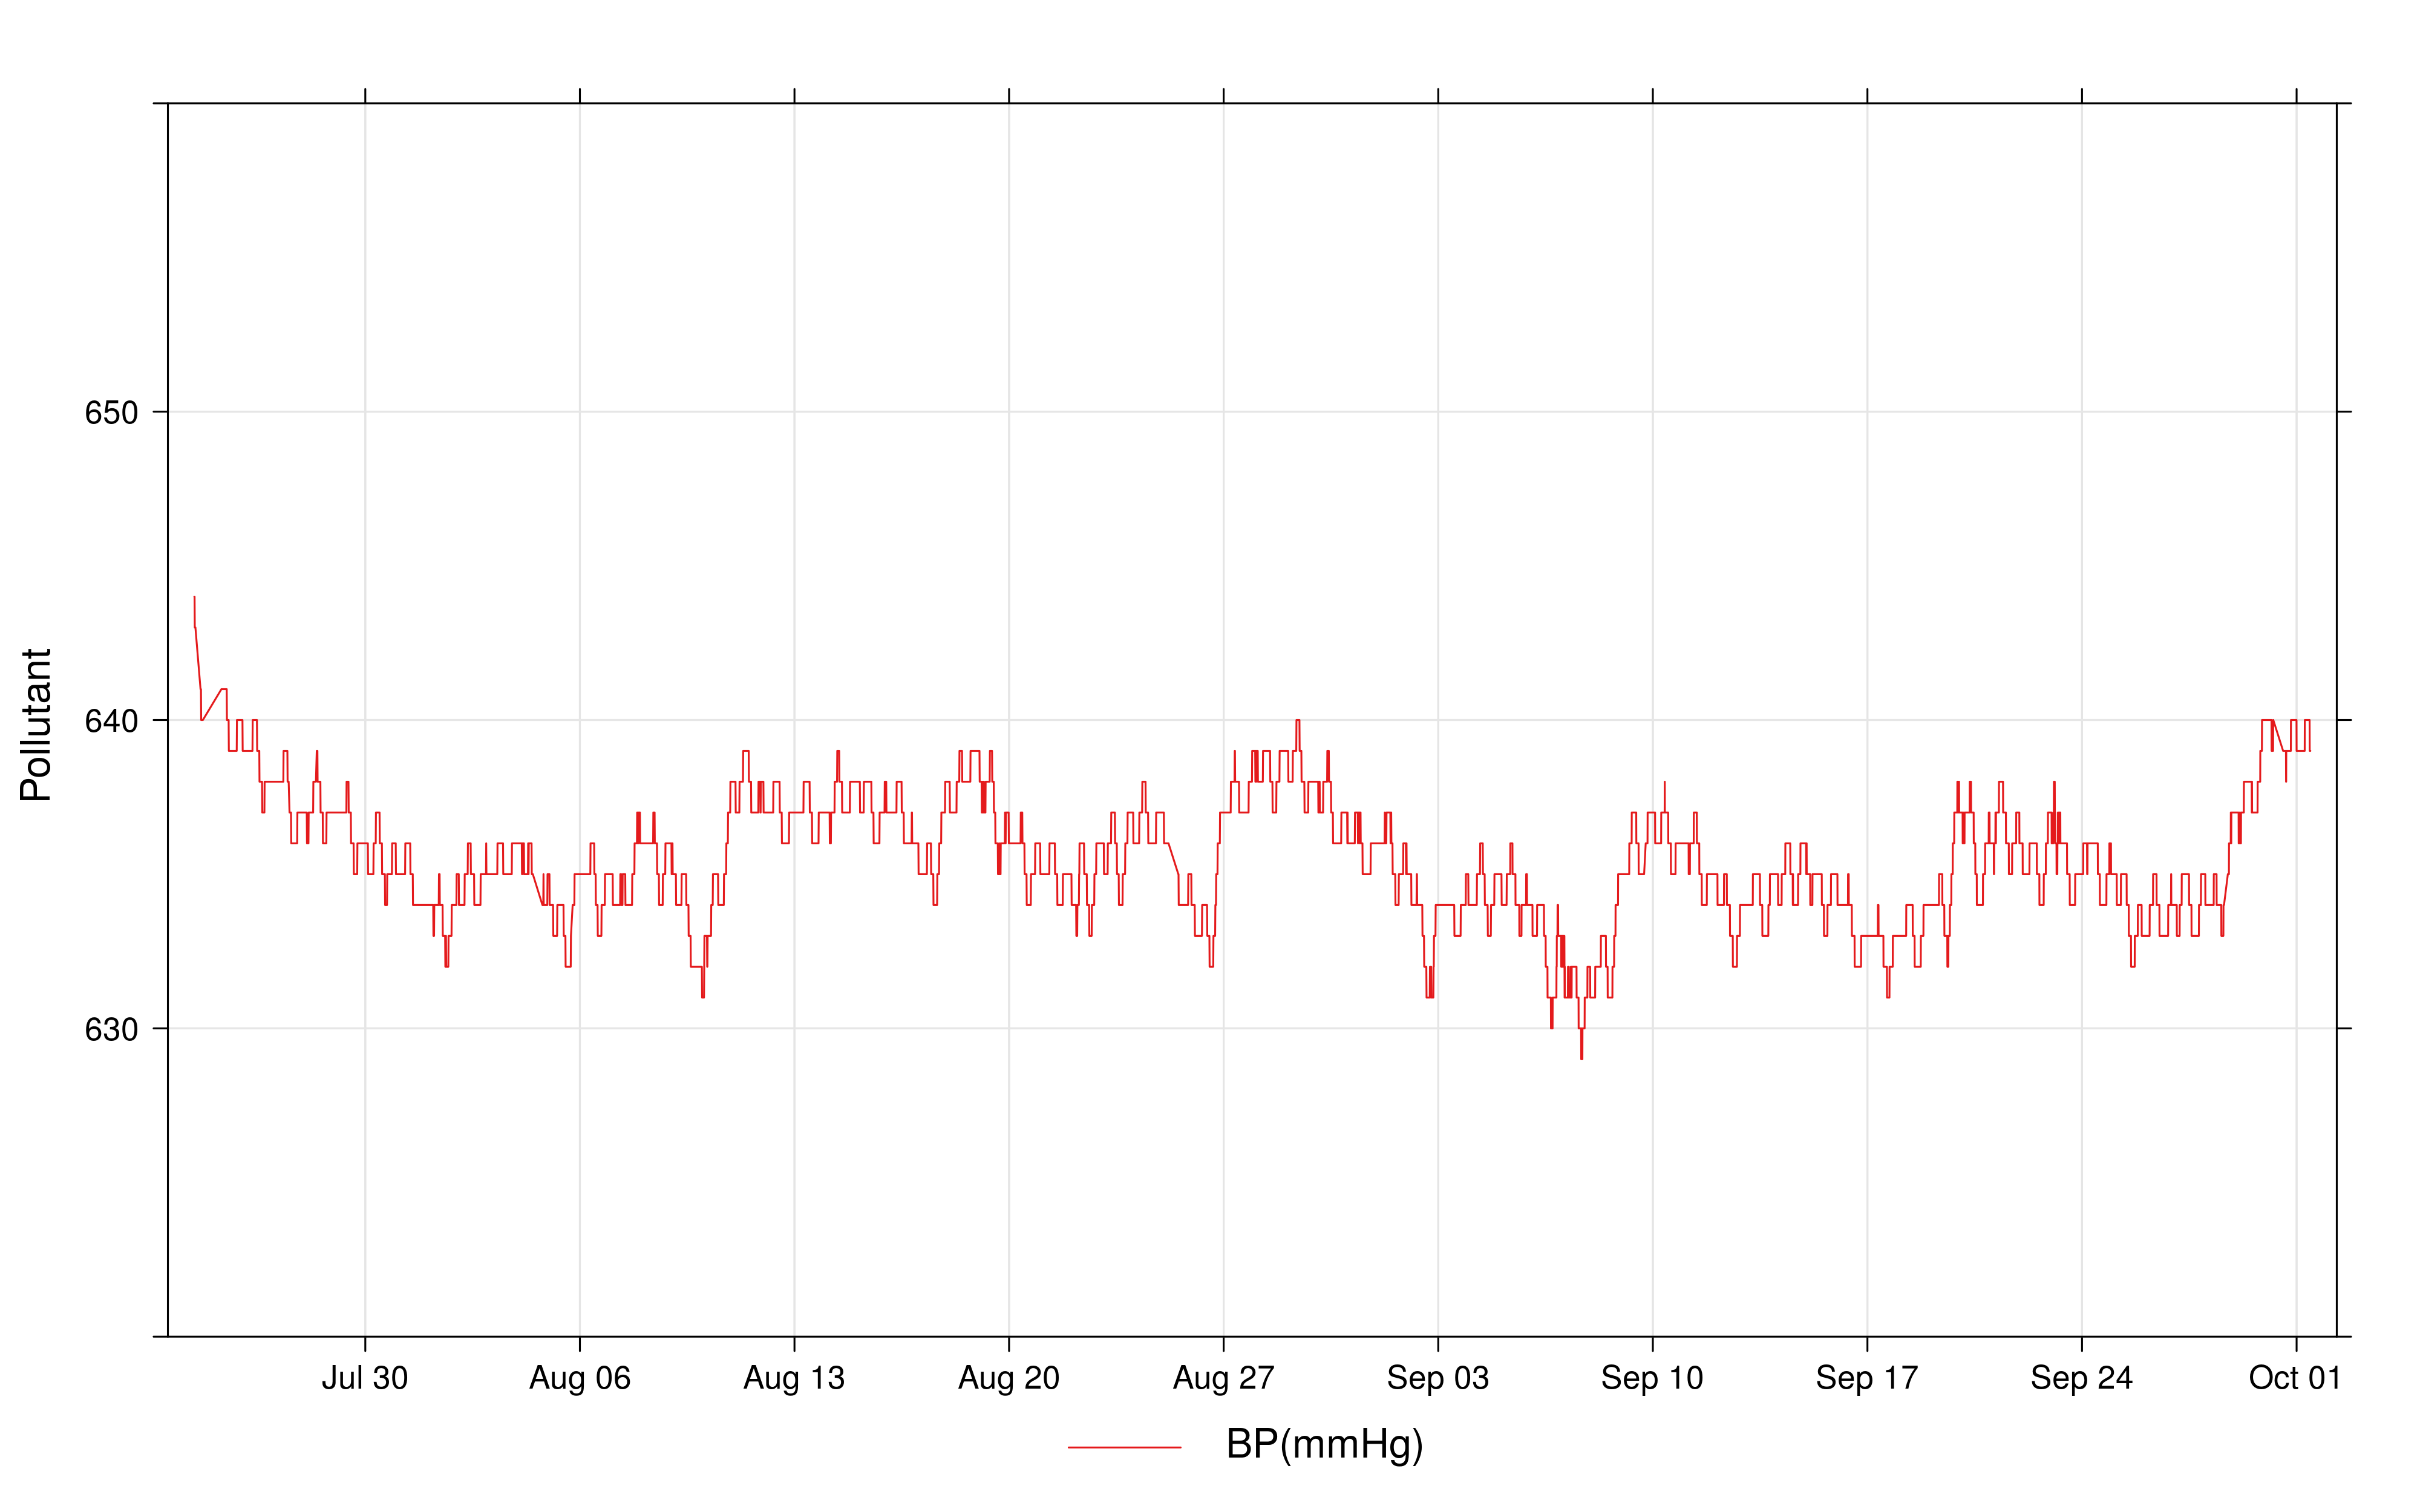
\includegraphics[width=\textwidth]{images/bp_timplt_25.png}
    \caption{Caption}
    \label{fig:pm2.5_BP_timplot}
\end{figure}

\begin{figure}[!htb]
    \centering
    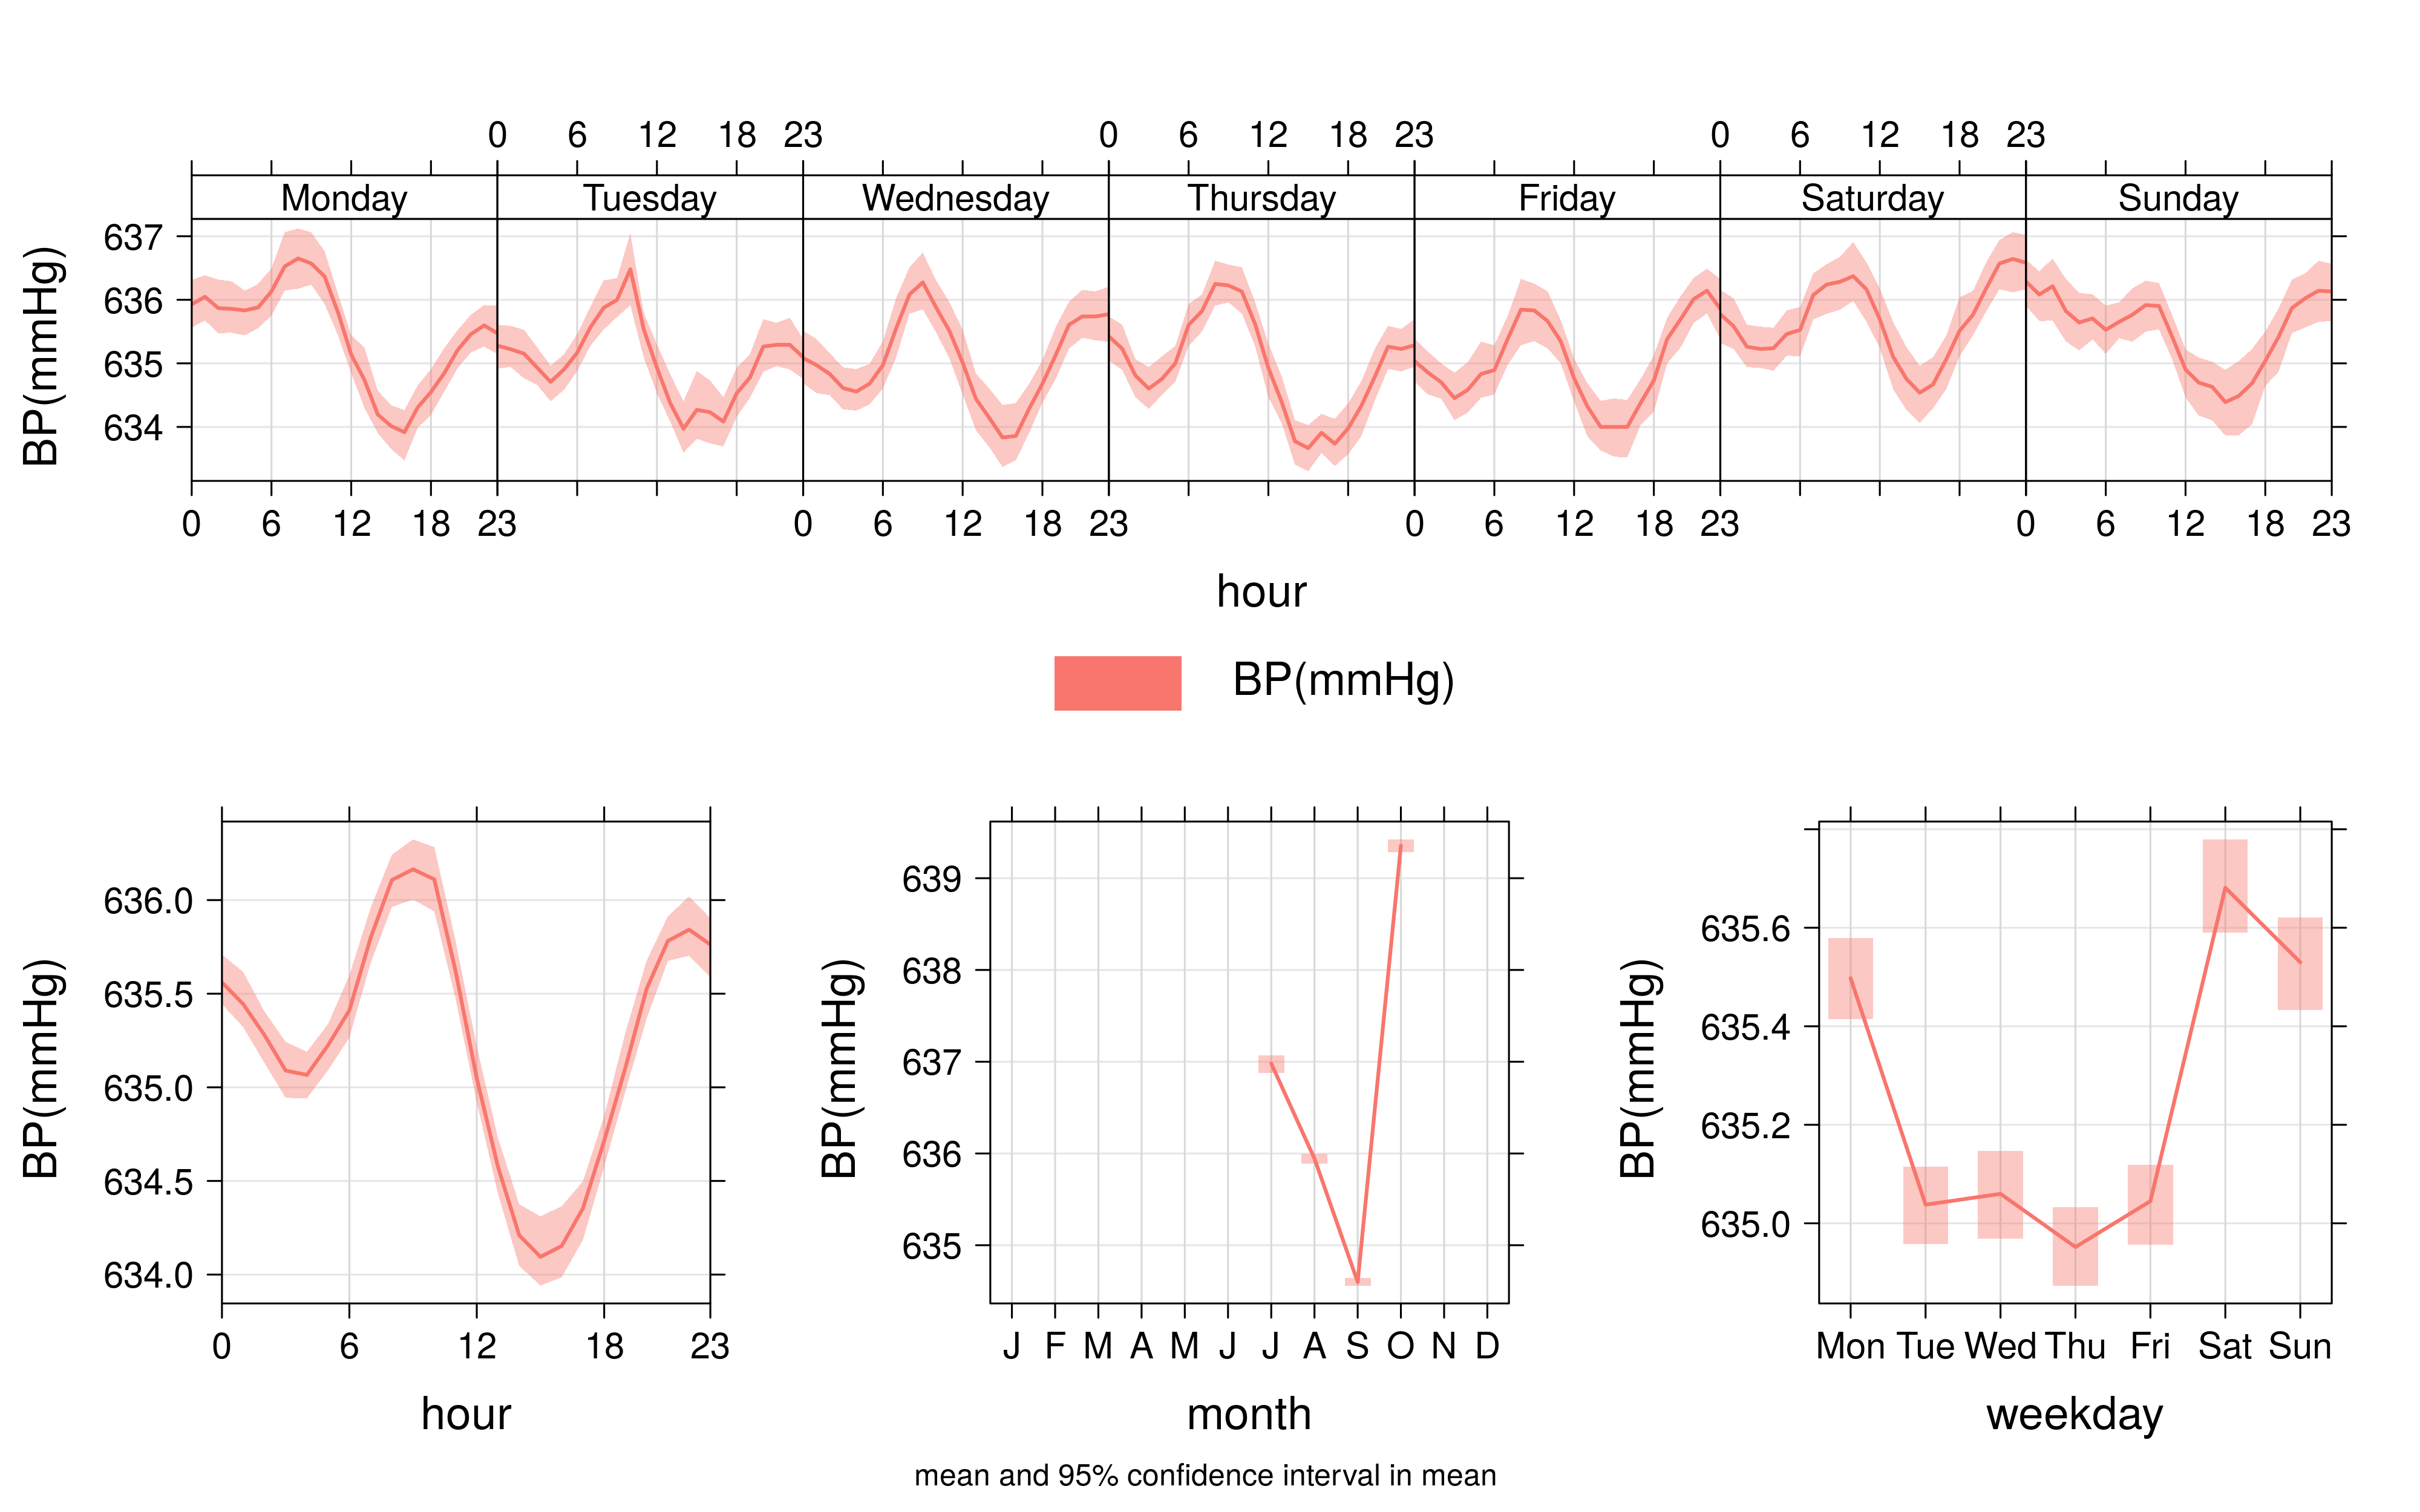
\includegraphics[width=\textwidth]{images/bp_25.png}
    \caption{Caption}
    \label{fig:pm2.5_BP}
\end{figure}

\begin{figure}[!htb]
    \centering
    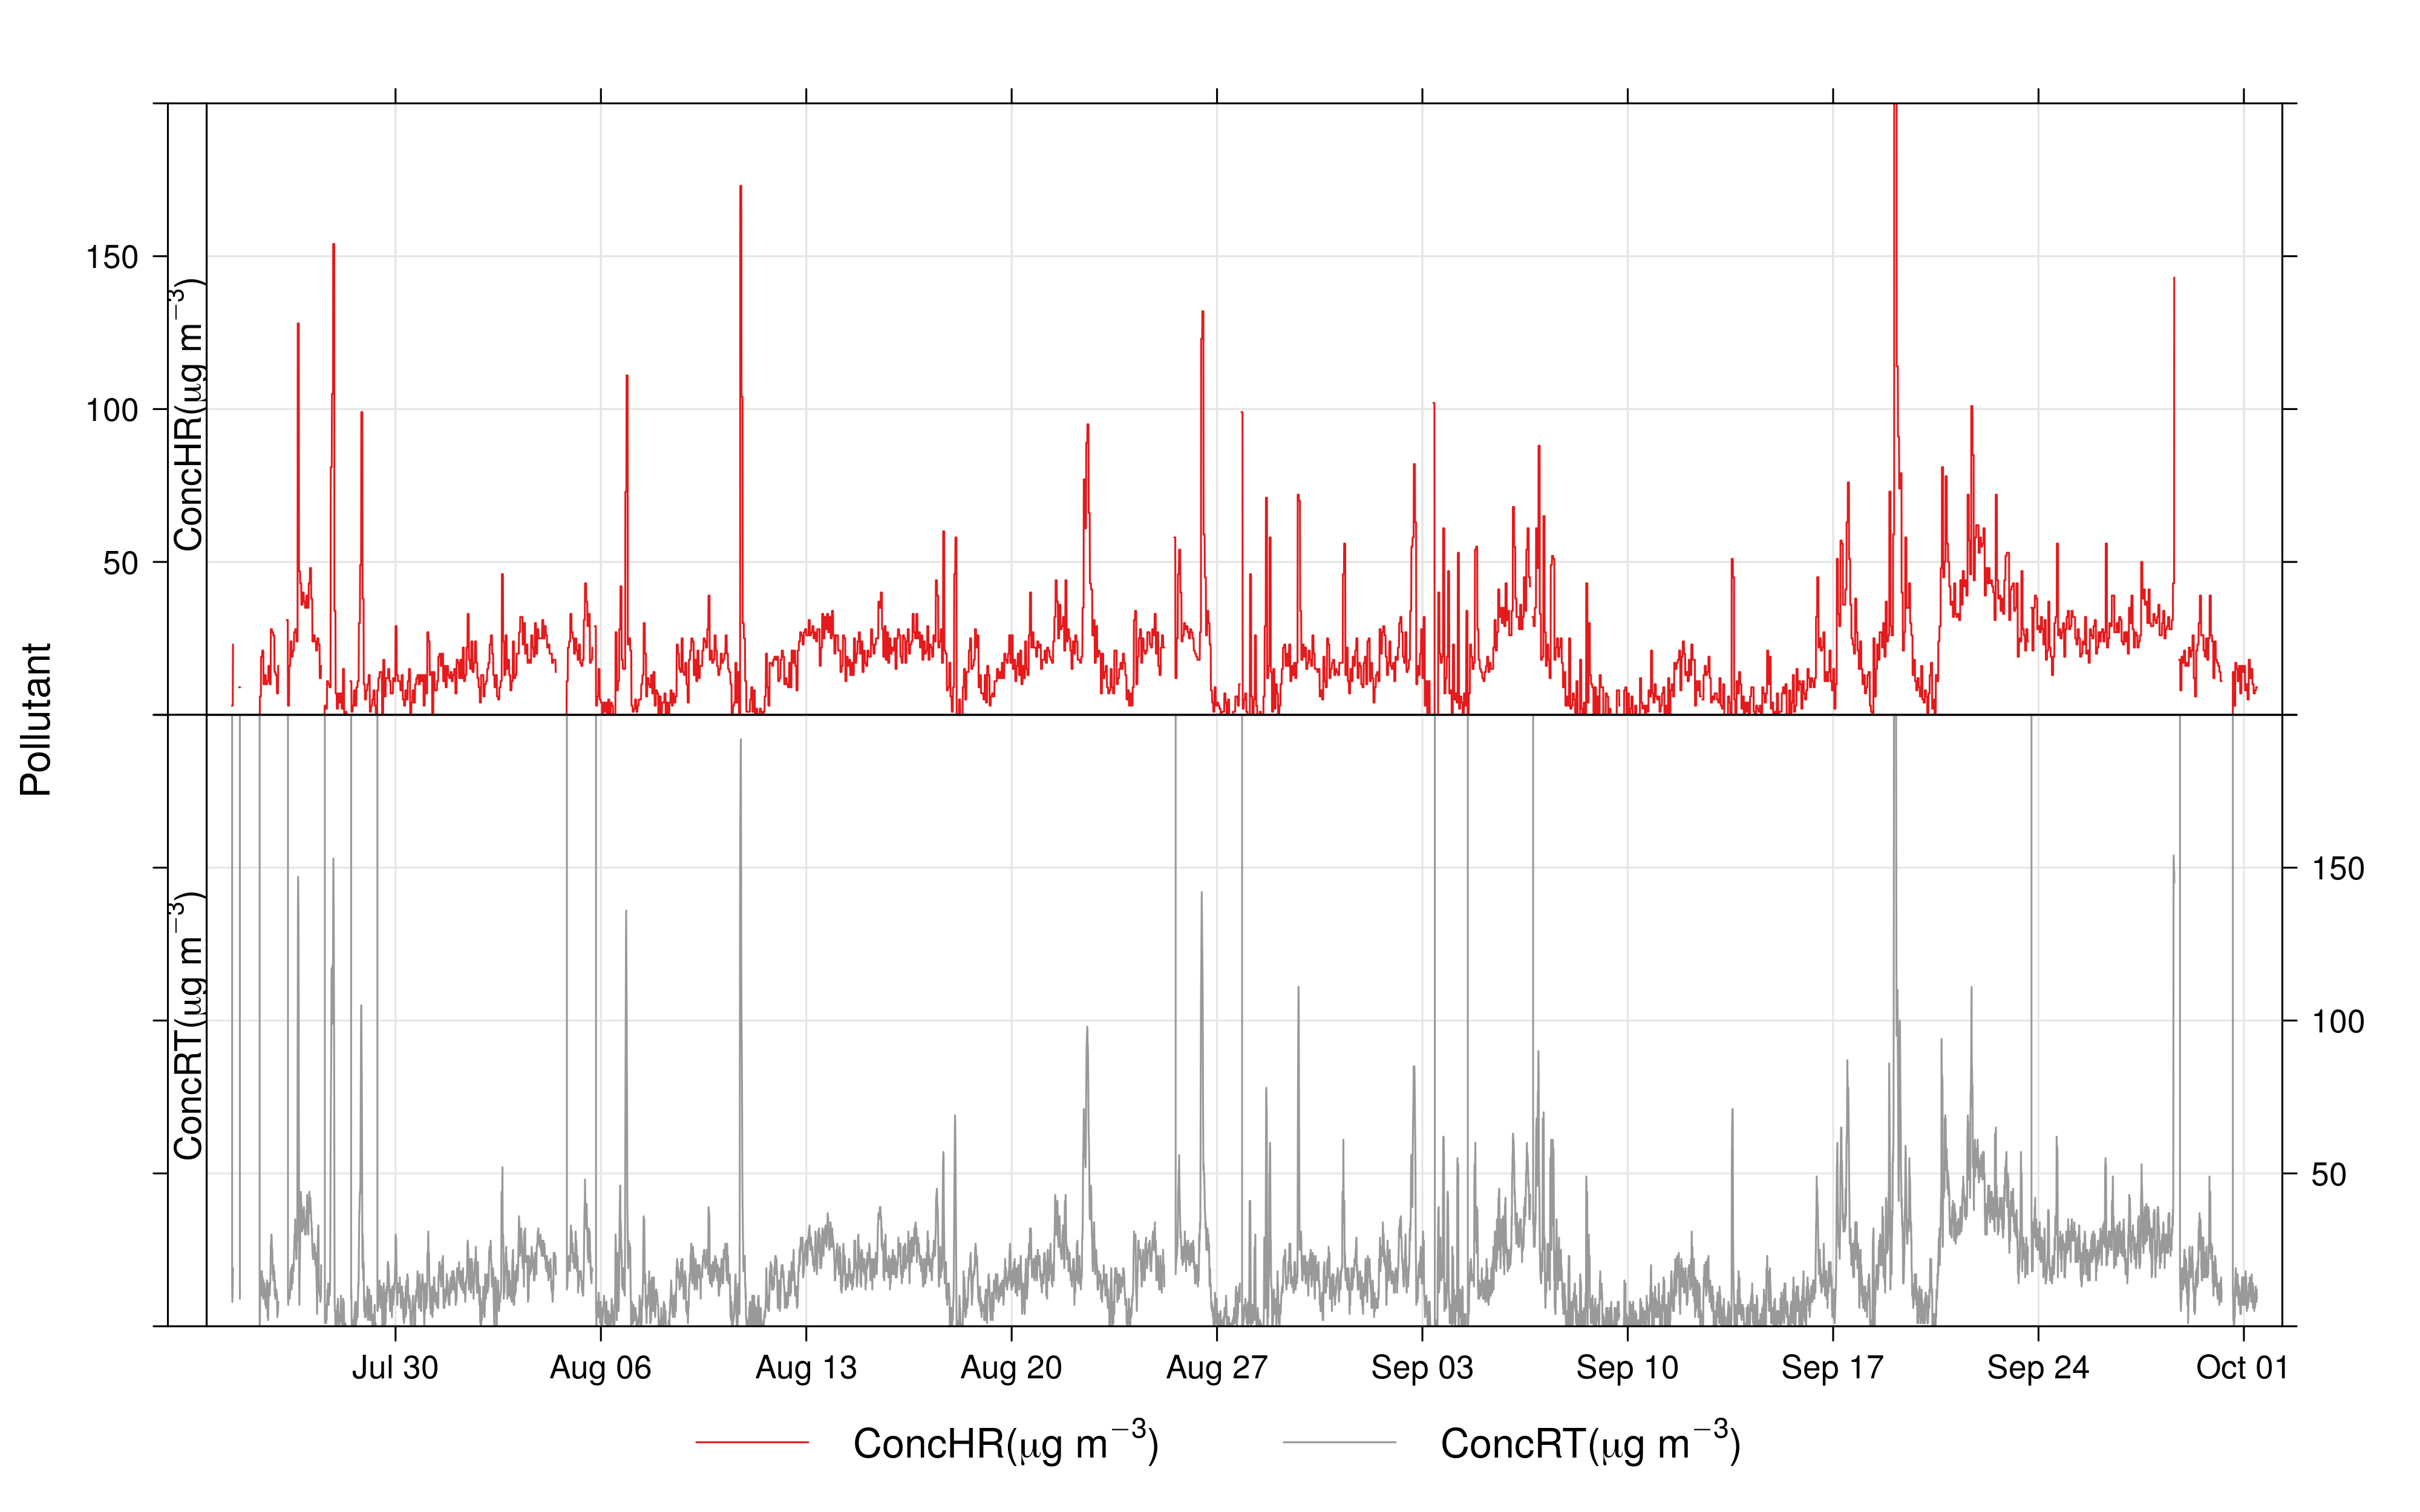
\includegraphics[width=\textwidth]{images/conc_timplt_25.png}
    \caption{Caption}
    \label{fig:pm2.5conc_timeplot}
\end{figure}

\begin{figure}[!htb]
    \centering
    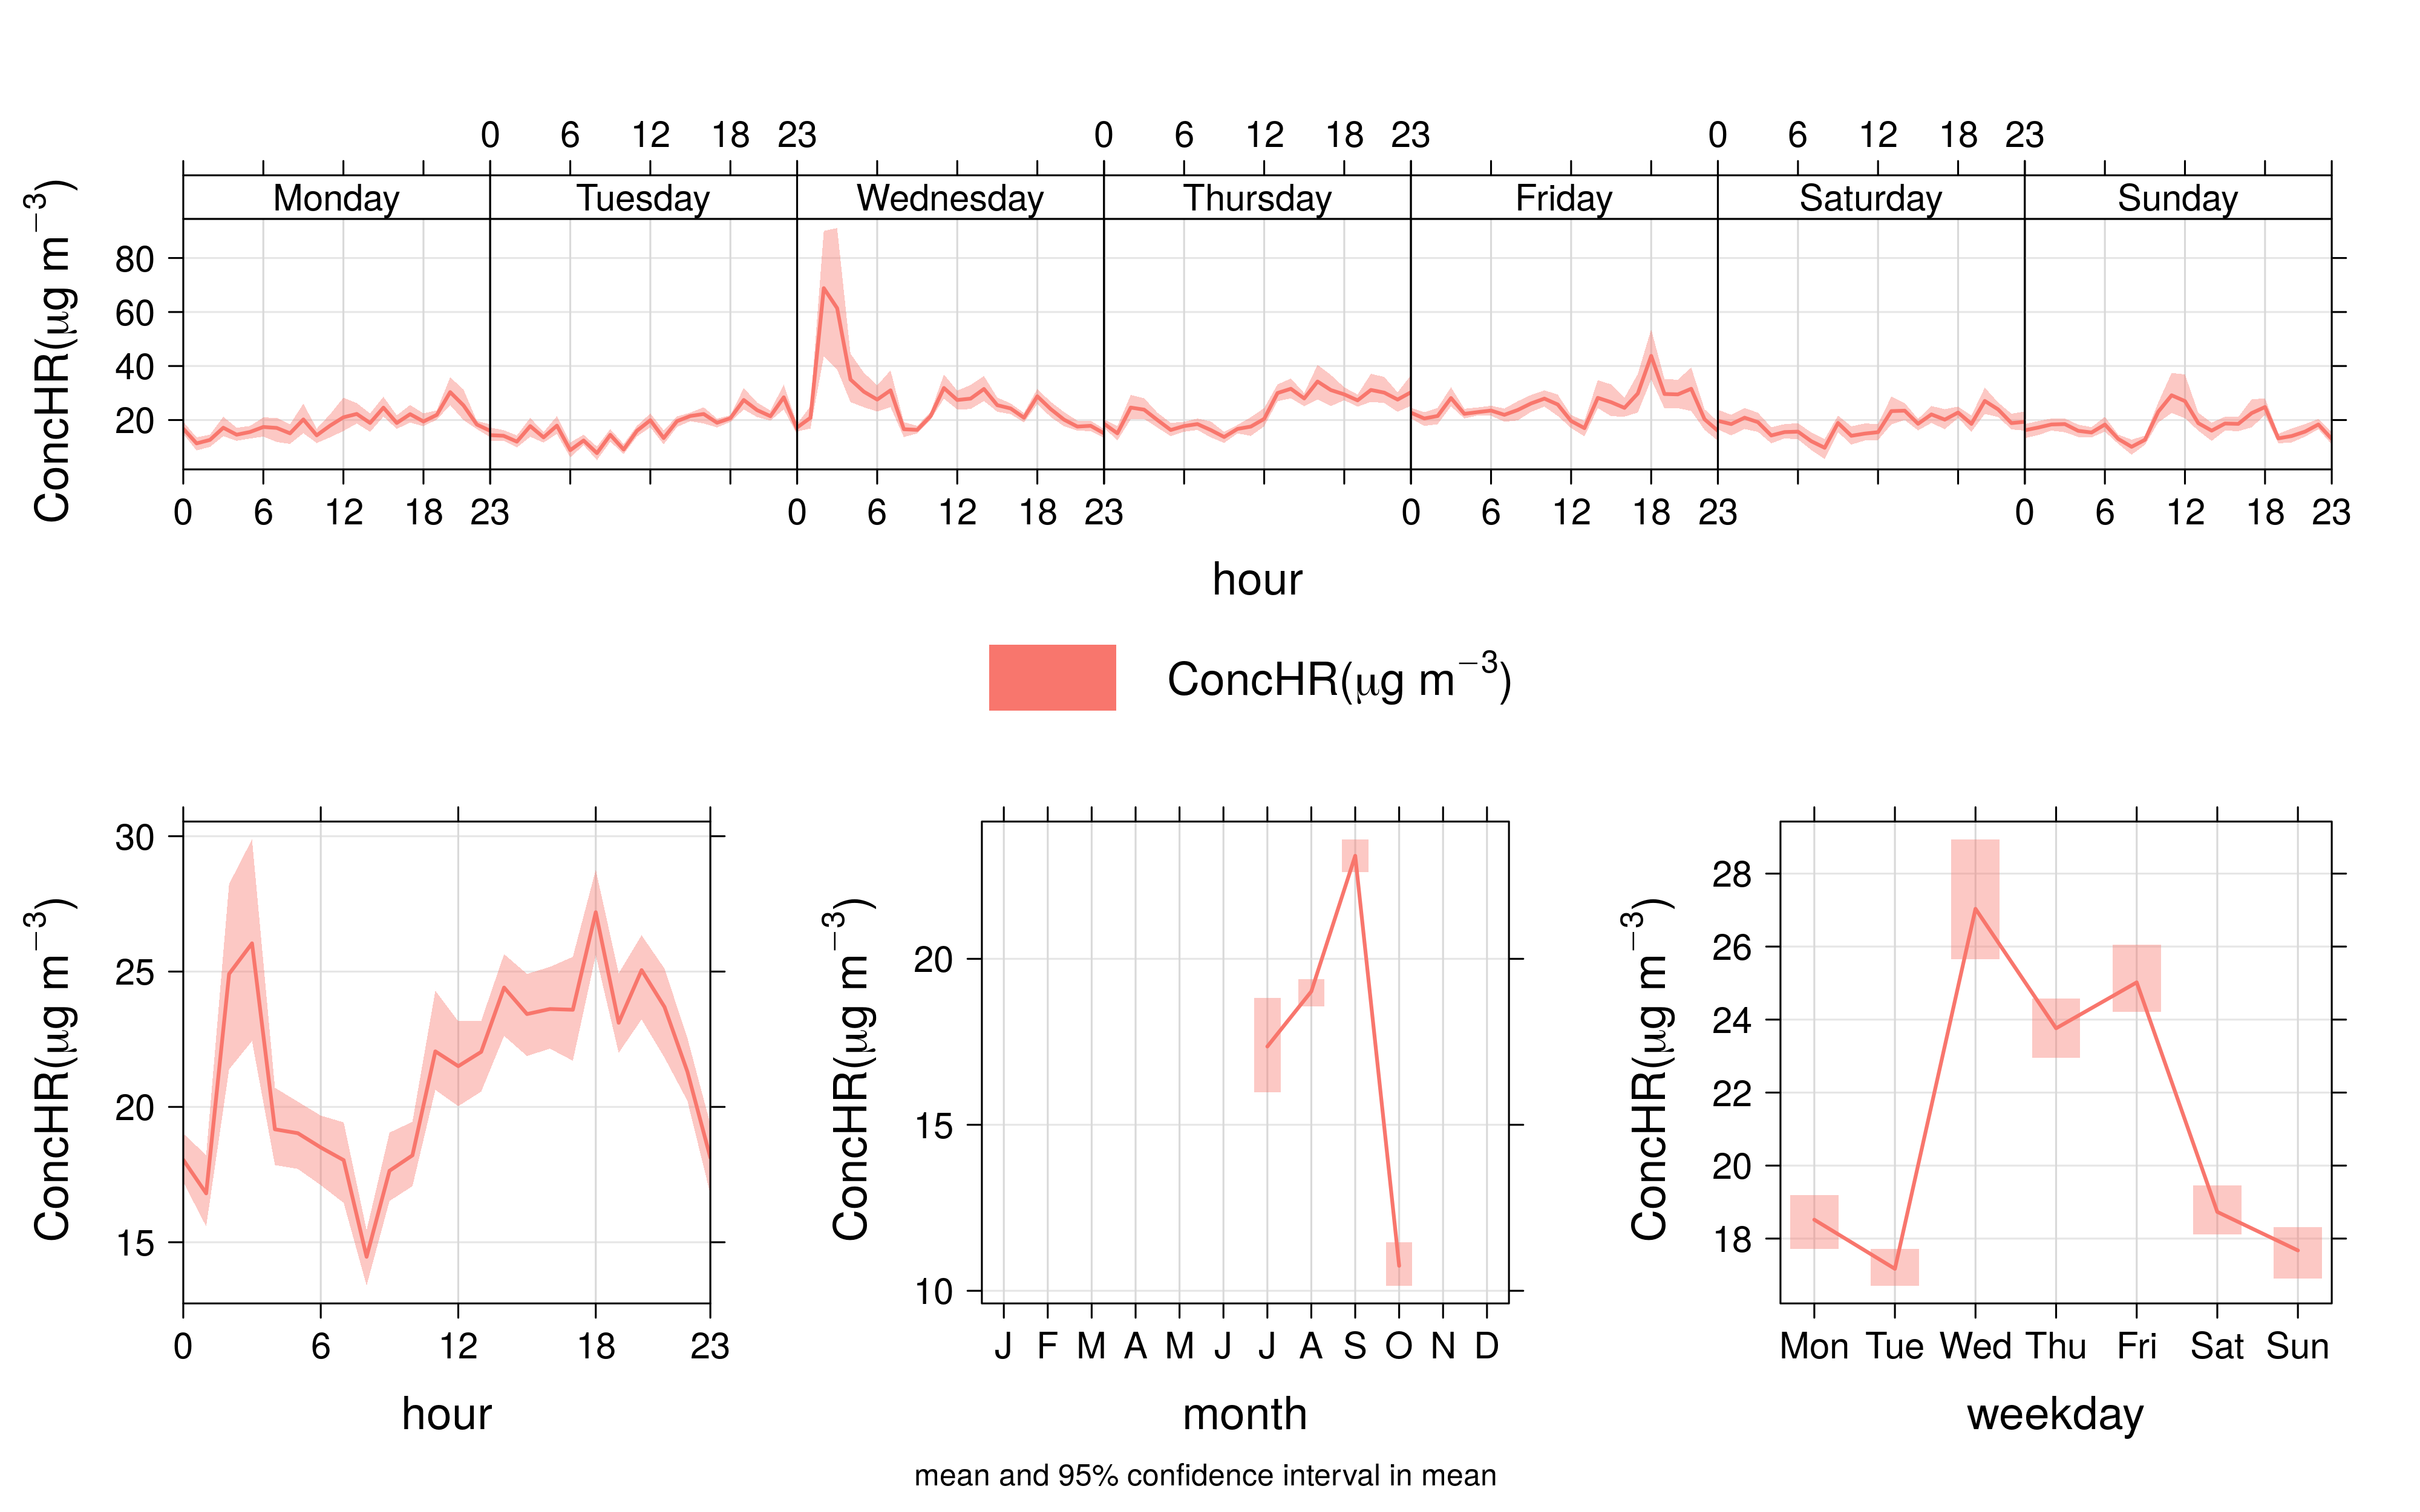
\includegraphics[width=\textwidth]{images/conc_HR_25.png}
    \caption{Caption}
    \label{fig:pm2.5conc_HR}
\end{figure}

\begin{figure}[!htb]
    \centering
    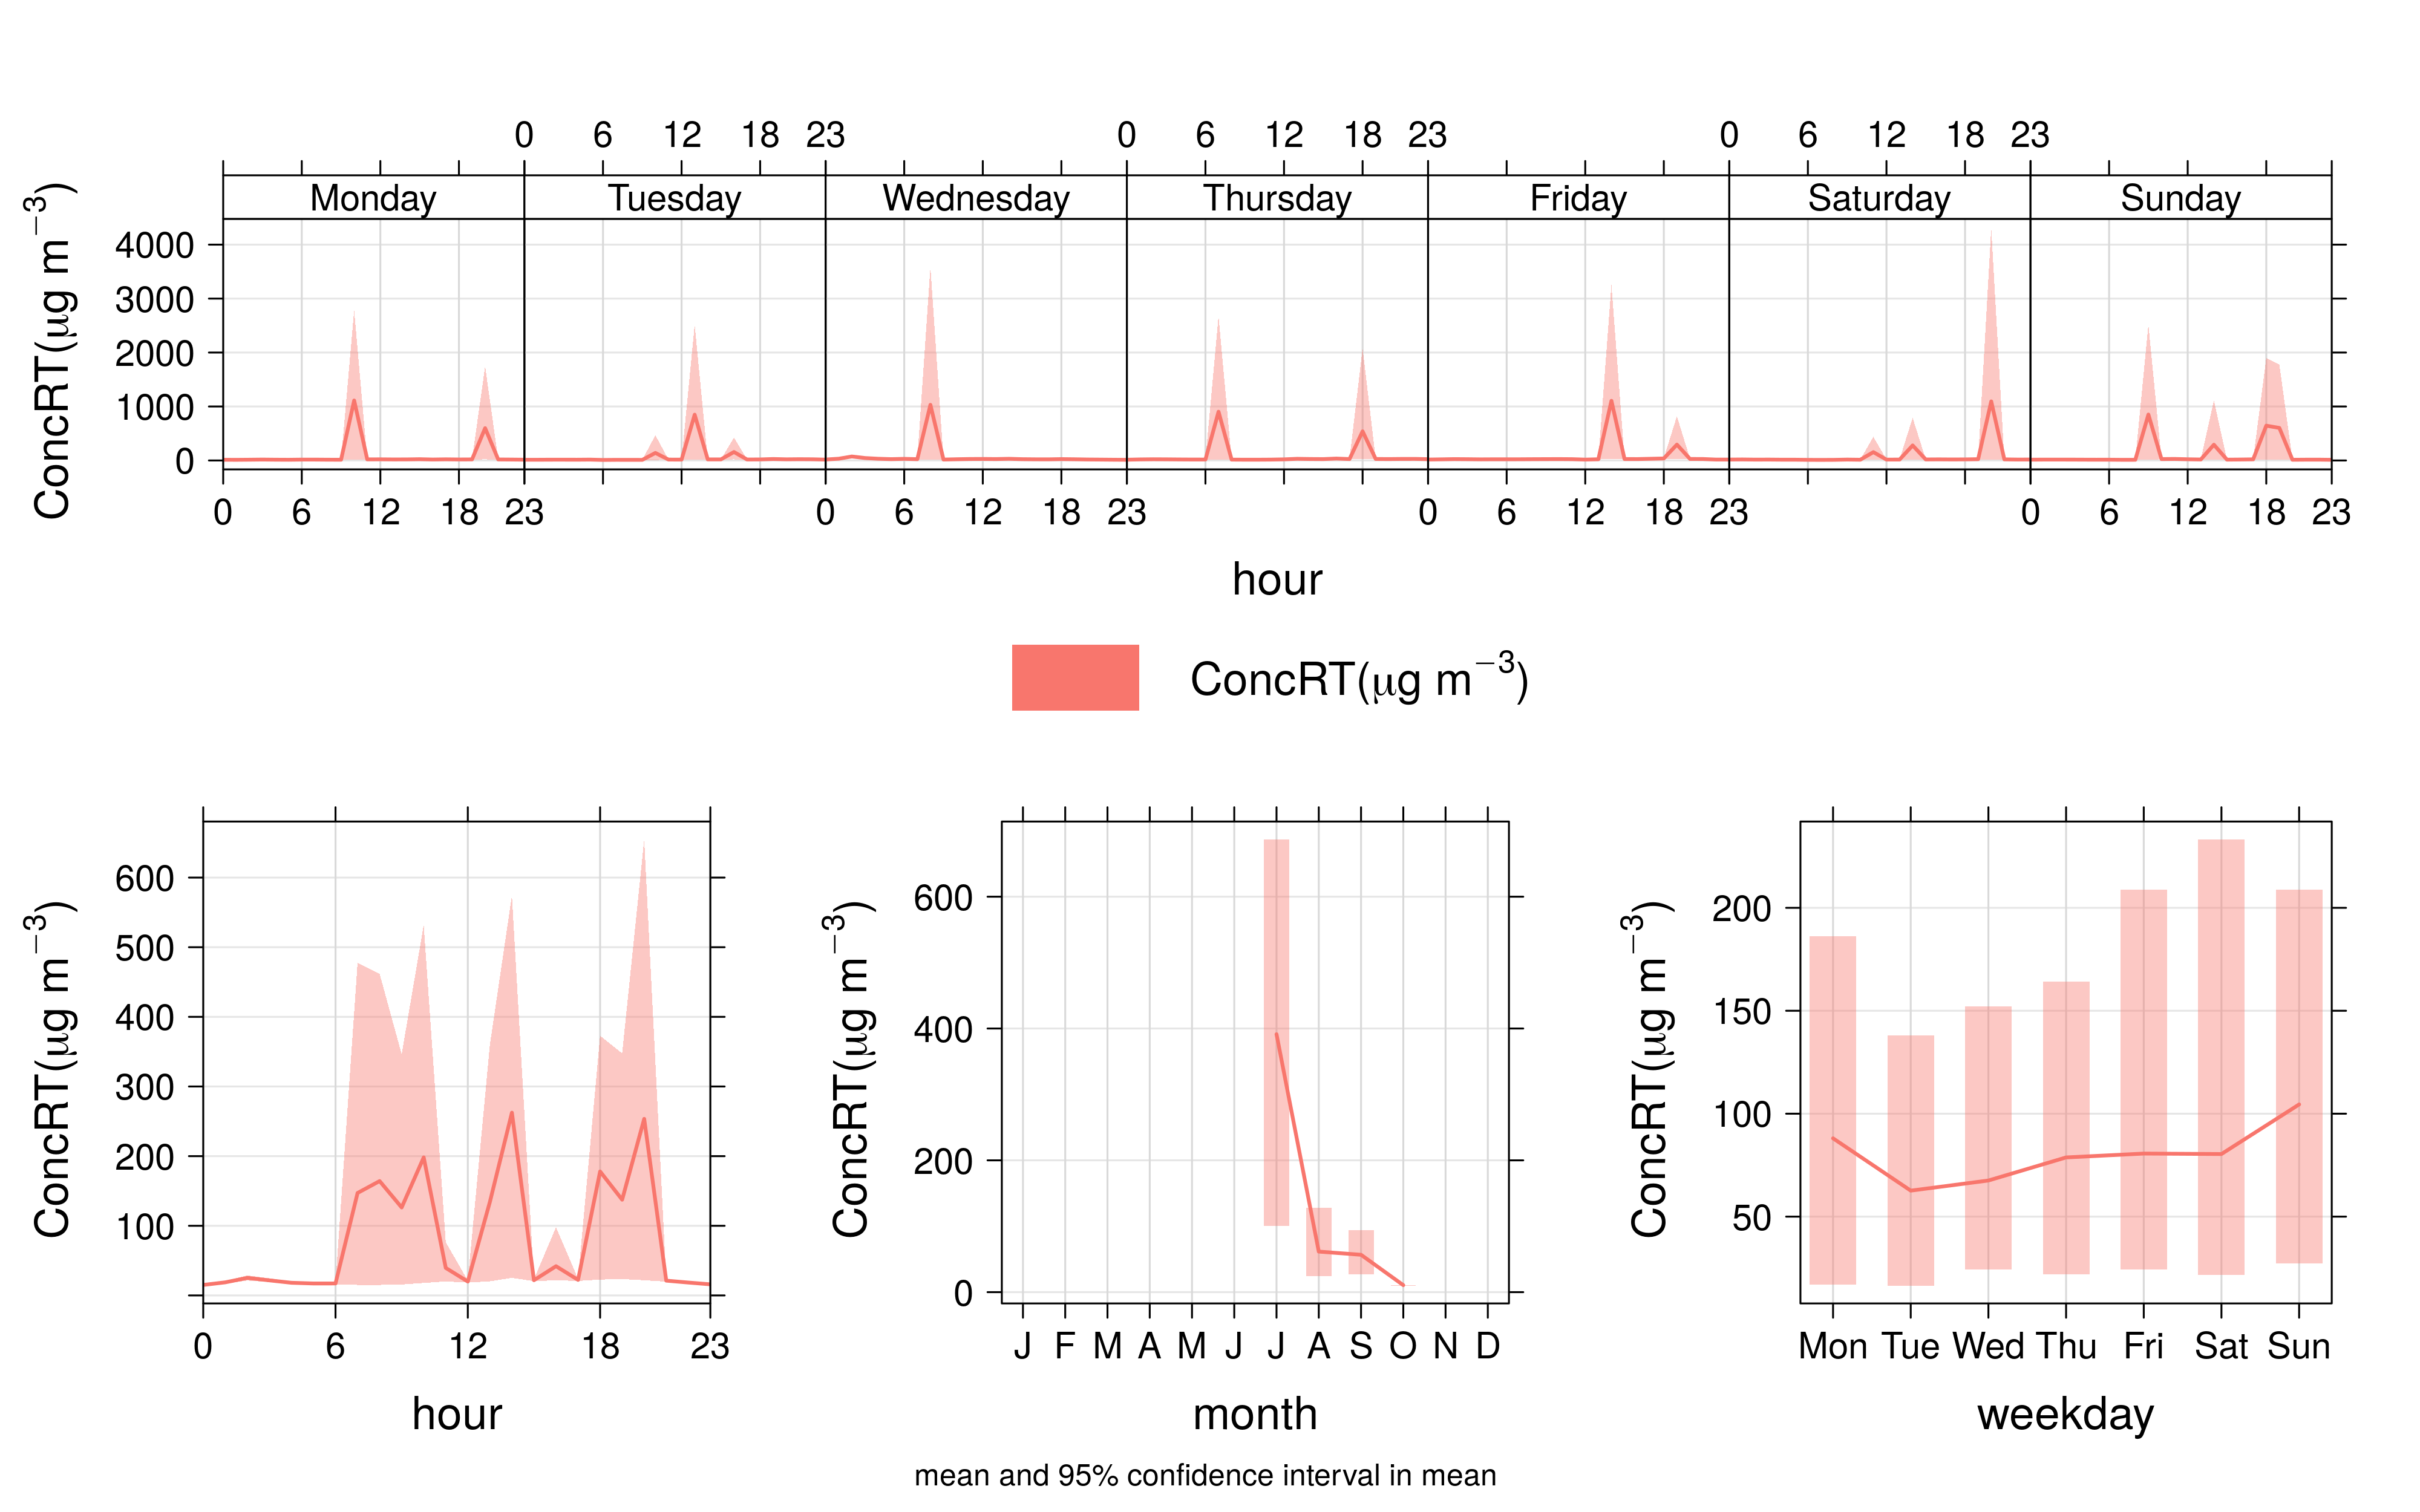
\includegraphics[width=\textwidth]{images/conc_RT_25.png}
    \caption{Caption}
    \label{fig:pm2.5conc_RT}
\end{figure}

\begin{figure}[!htb]
    \centering
    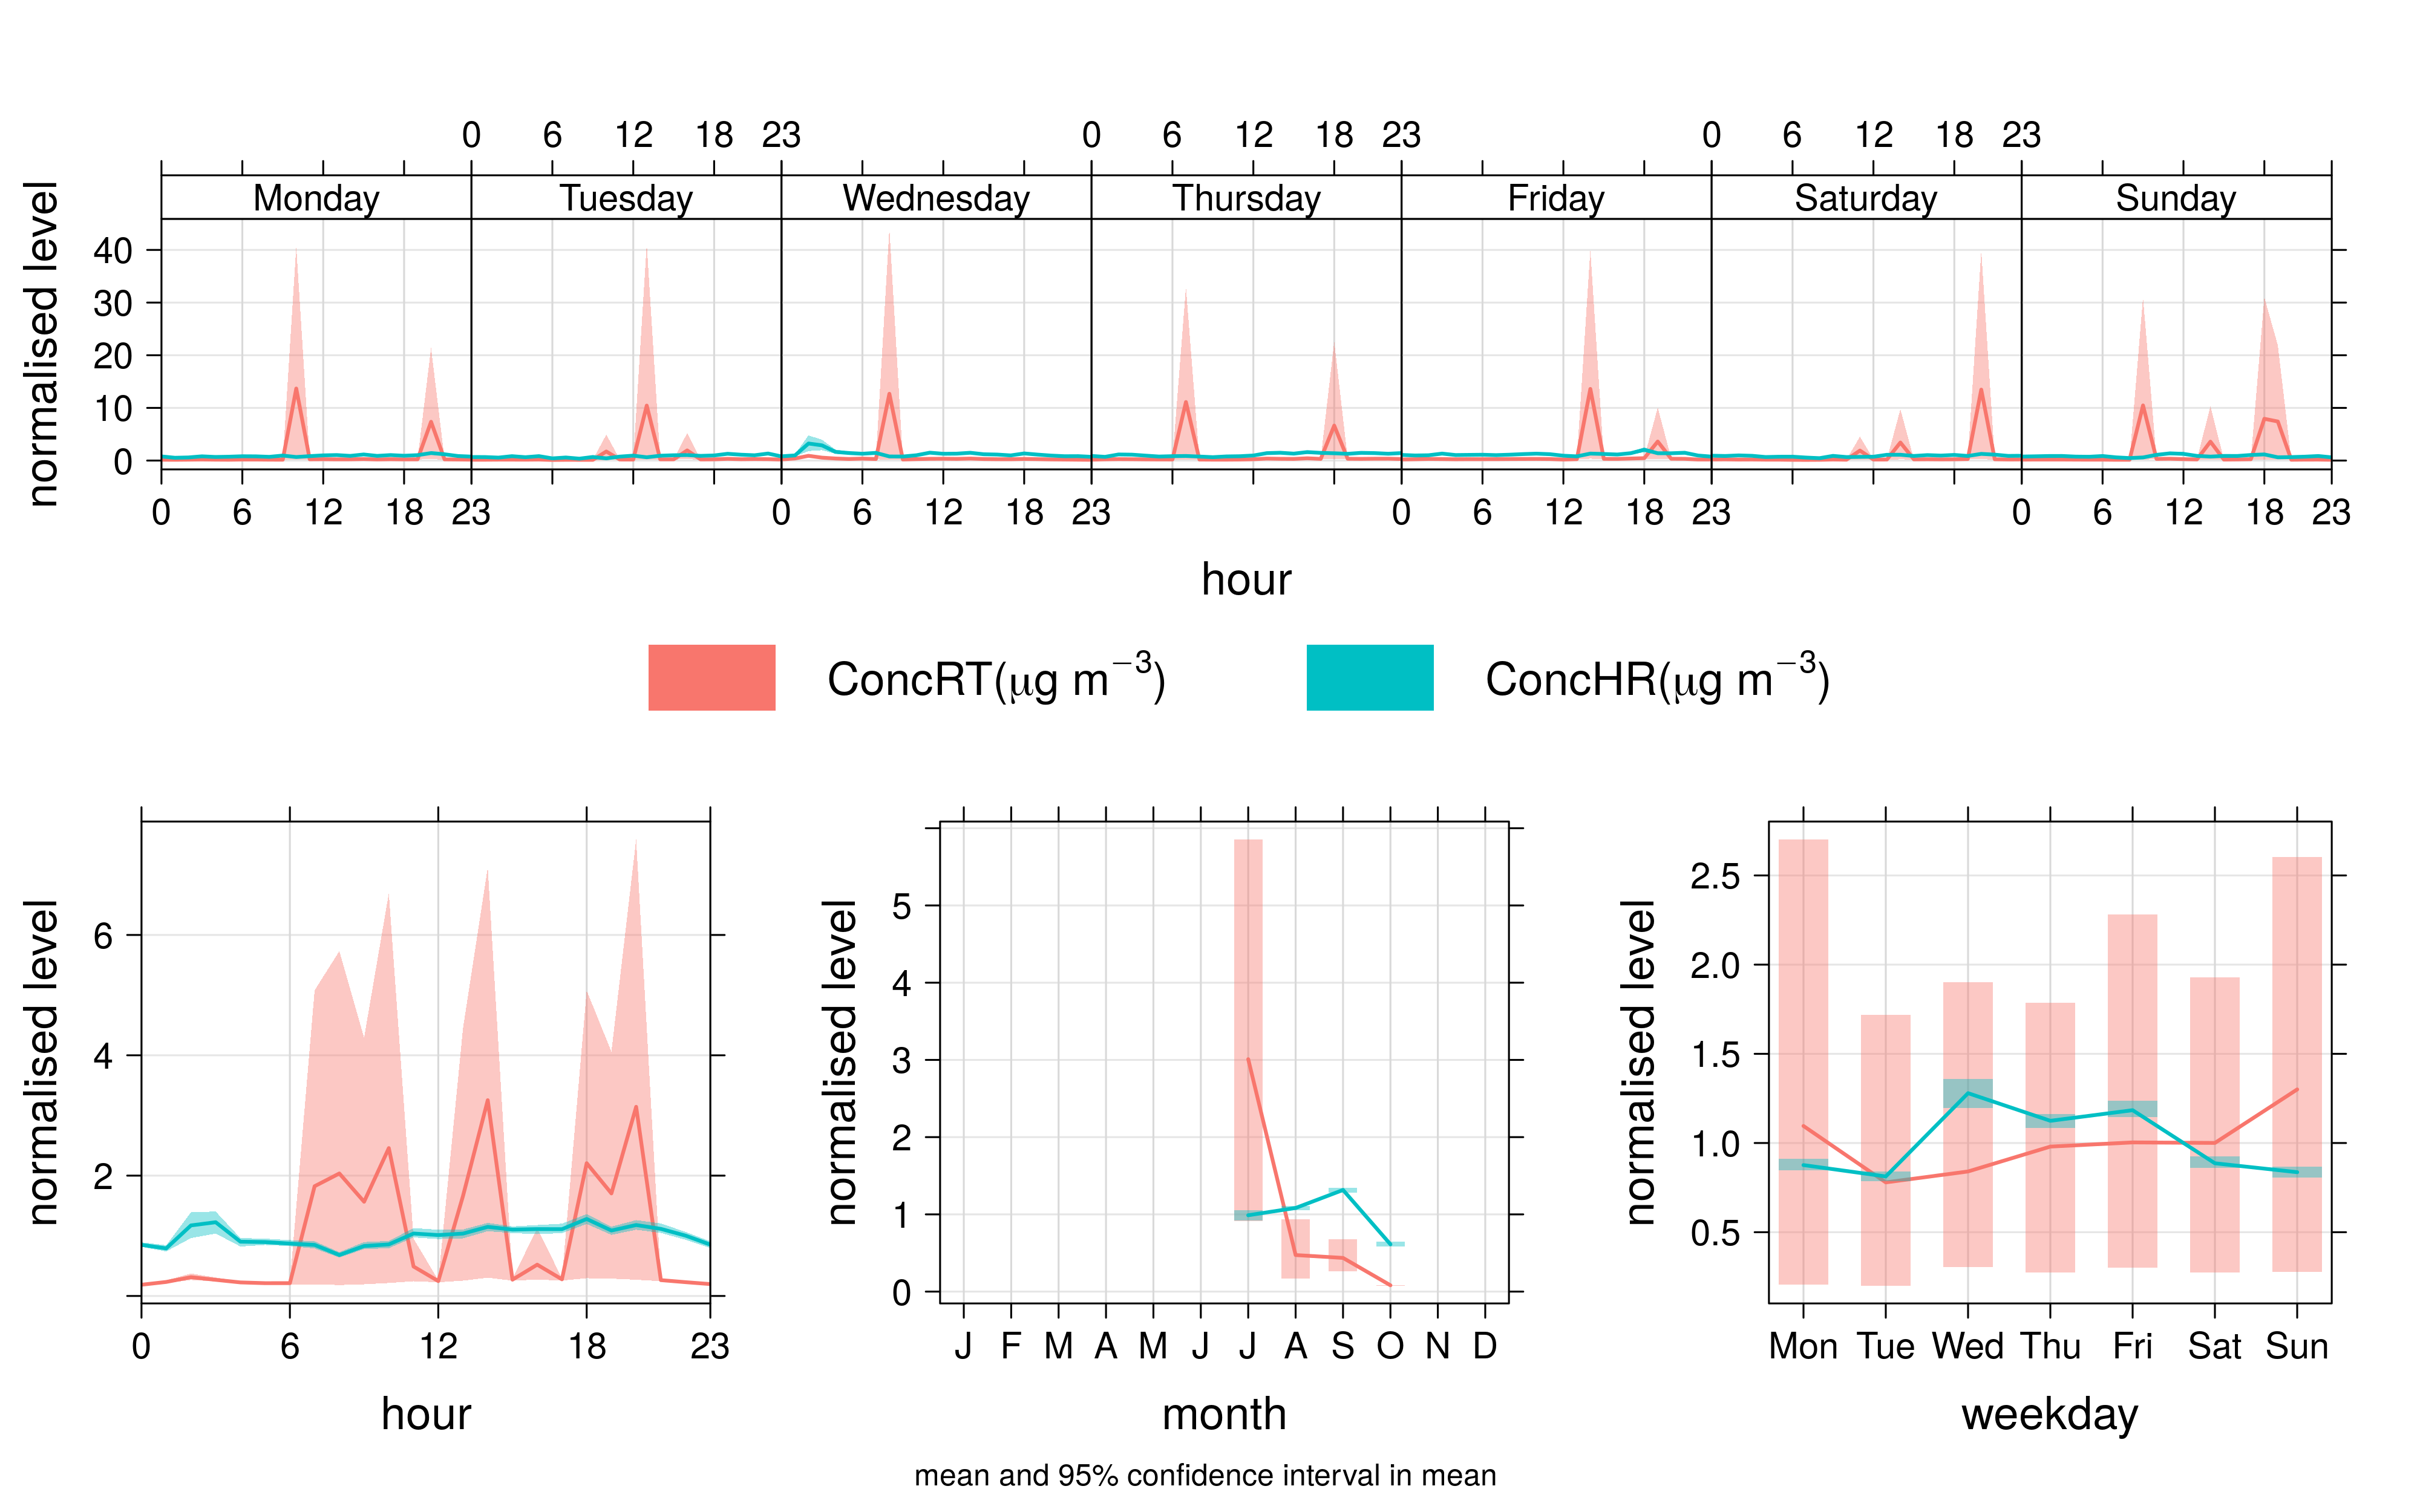
\includegraphics[width=\textwidth]{images/conc_25.png}
    \caption{Caption}
    \label{fig:pm2.5conc_all}
\end{figure}

\begin{figure}[!htb]
    \centering
    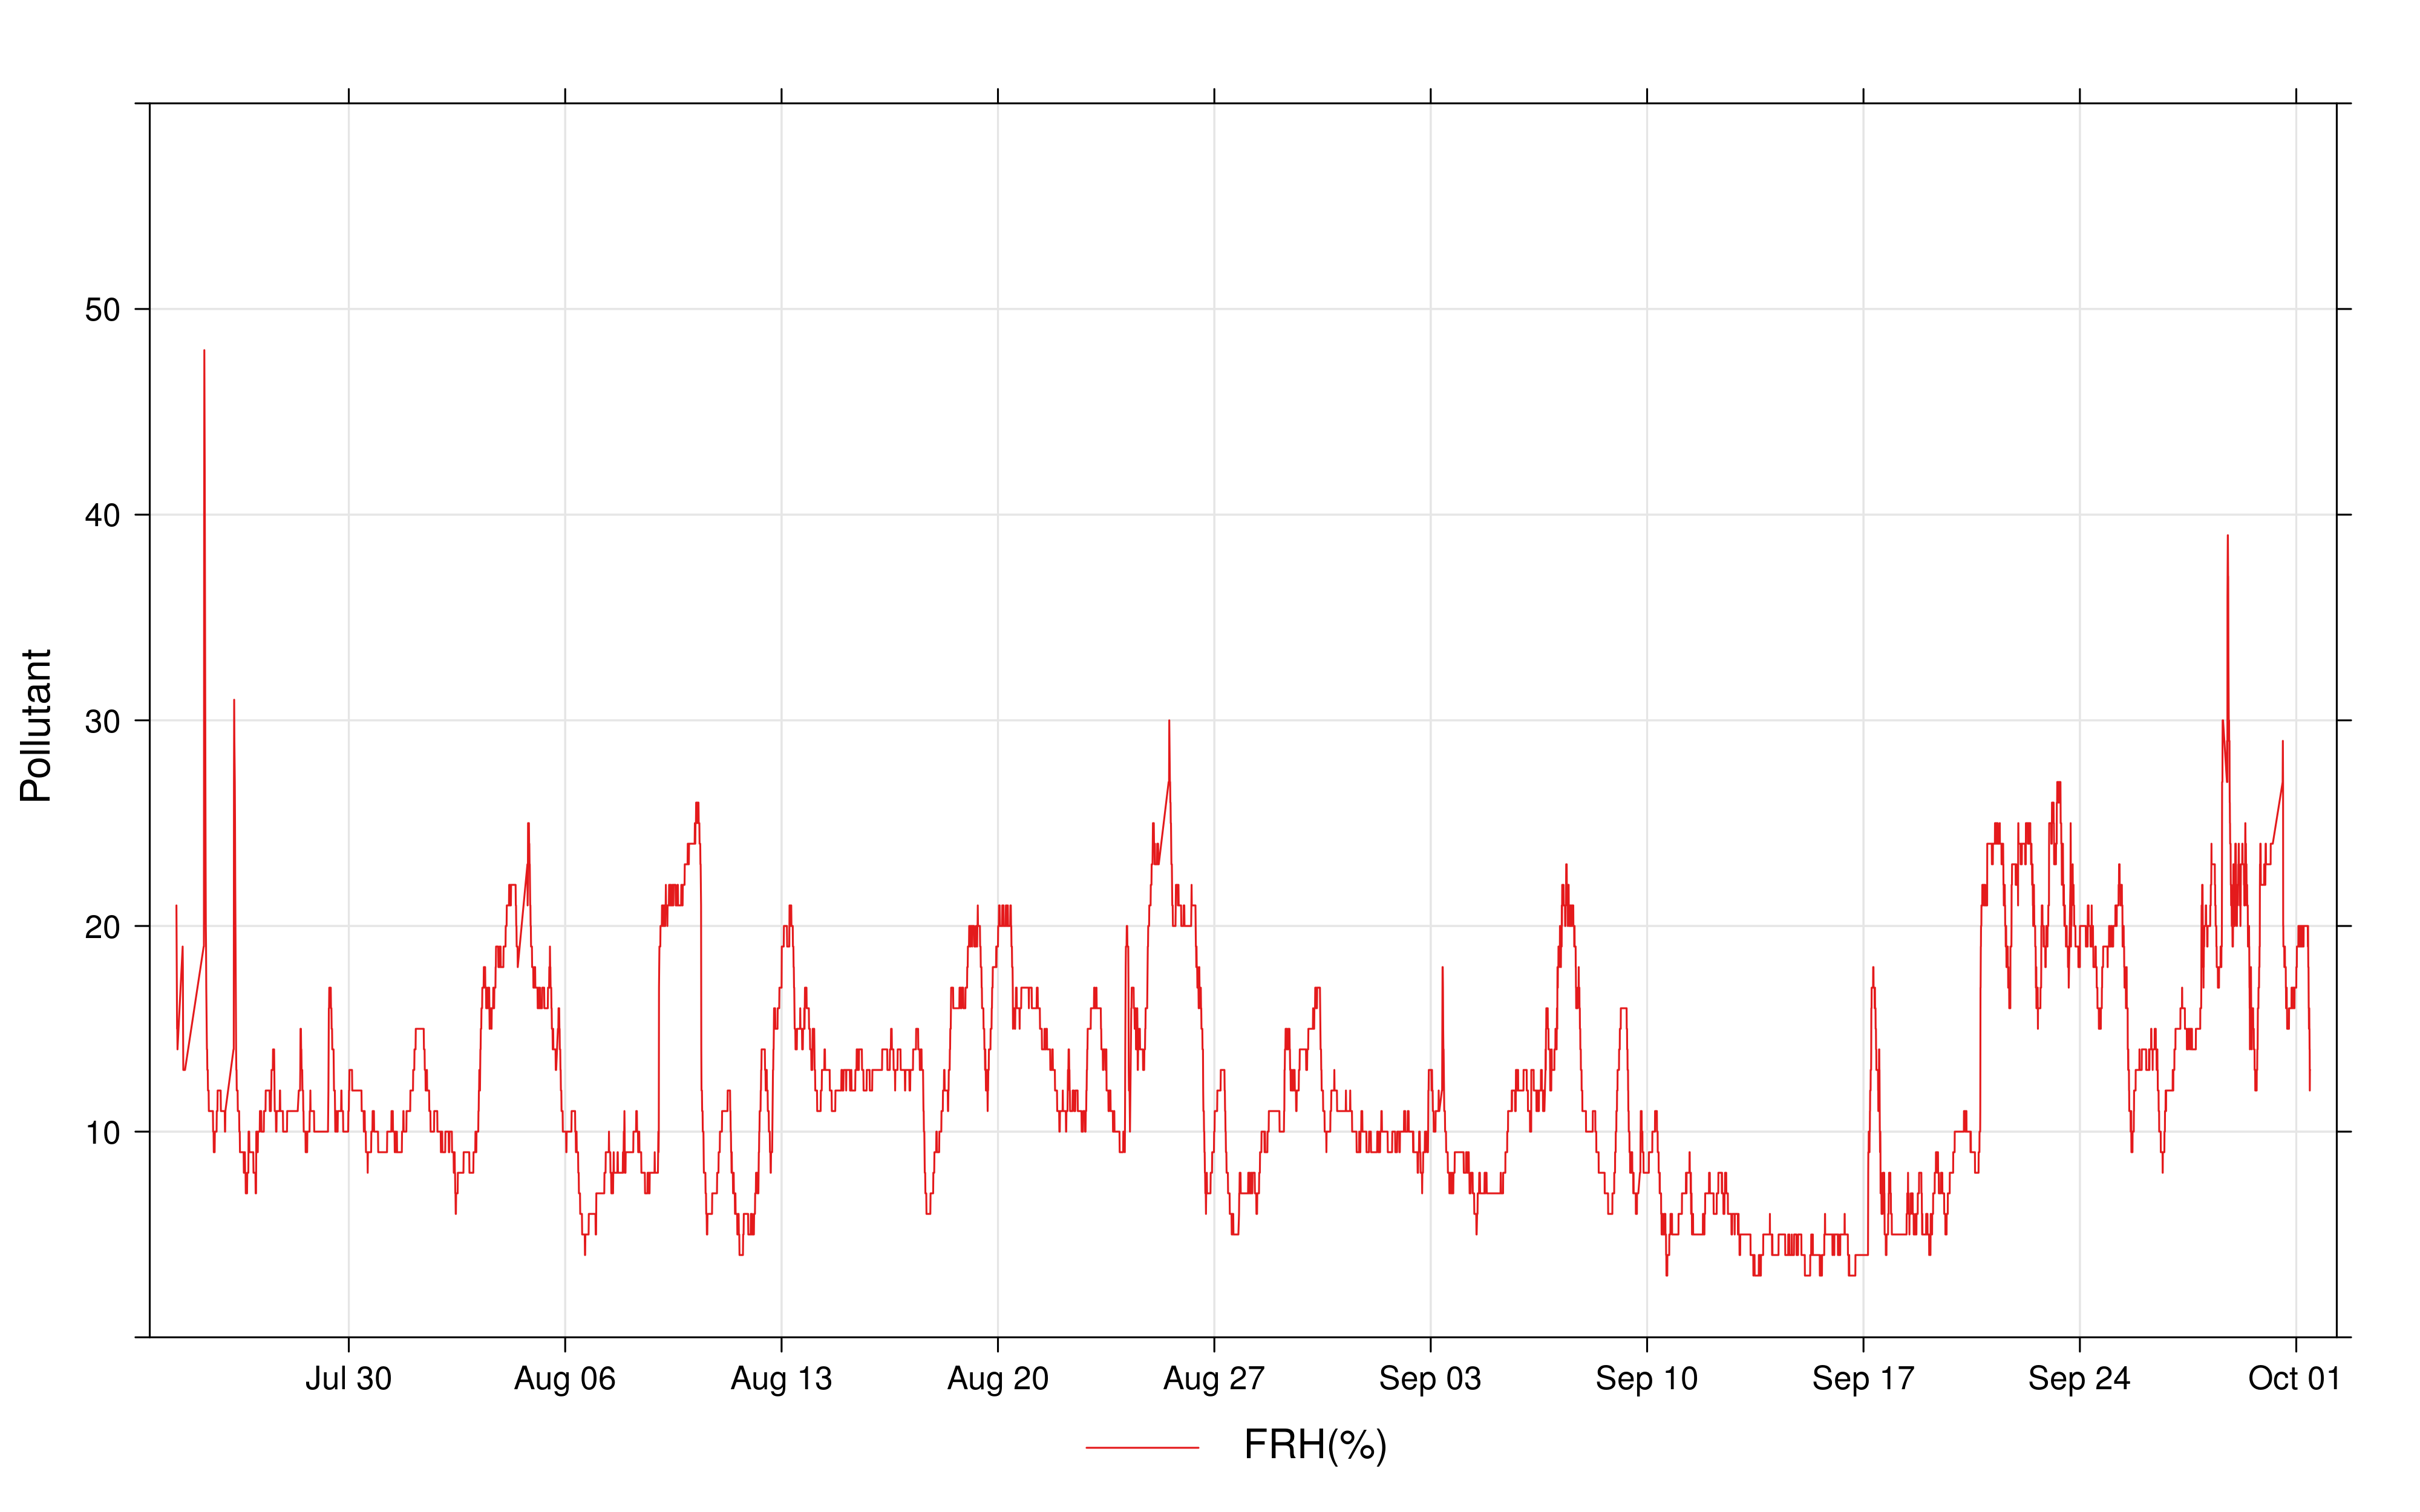
\includegraphics[width=\textwidth]{images/frh_timplt_25.png}}
    \caption{Caption}
    \label{fig:pm2.5_FR_timplot}
\end{figure}

%%%%%%%%%%%%%%%%%%%%%%%%%%%%%%%%%%%%%%%%%%%%%%%%%%%%%%%%%%%%%%%%

\begin{figure}[!htb]
    \centering
    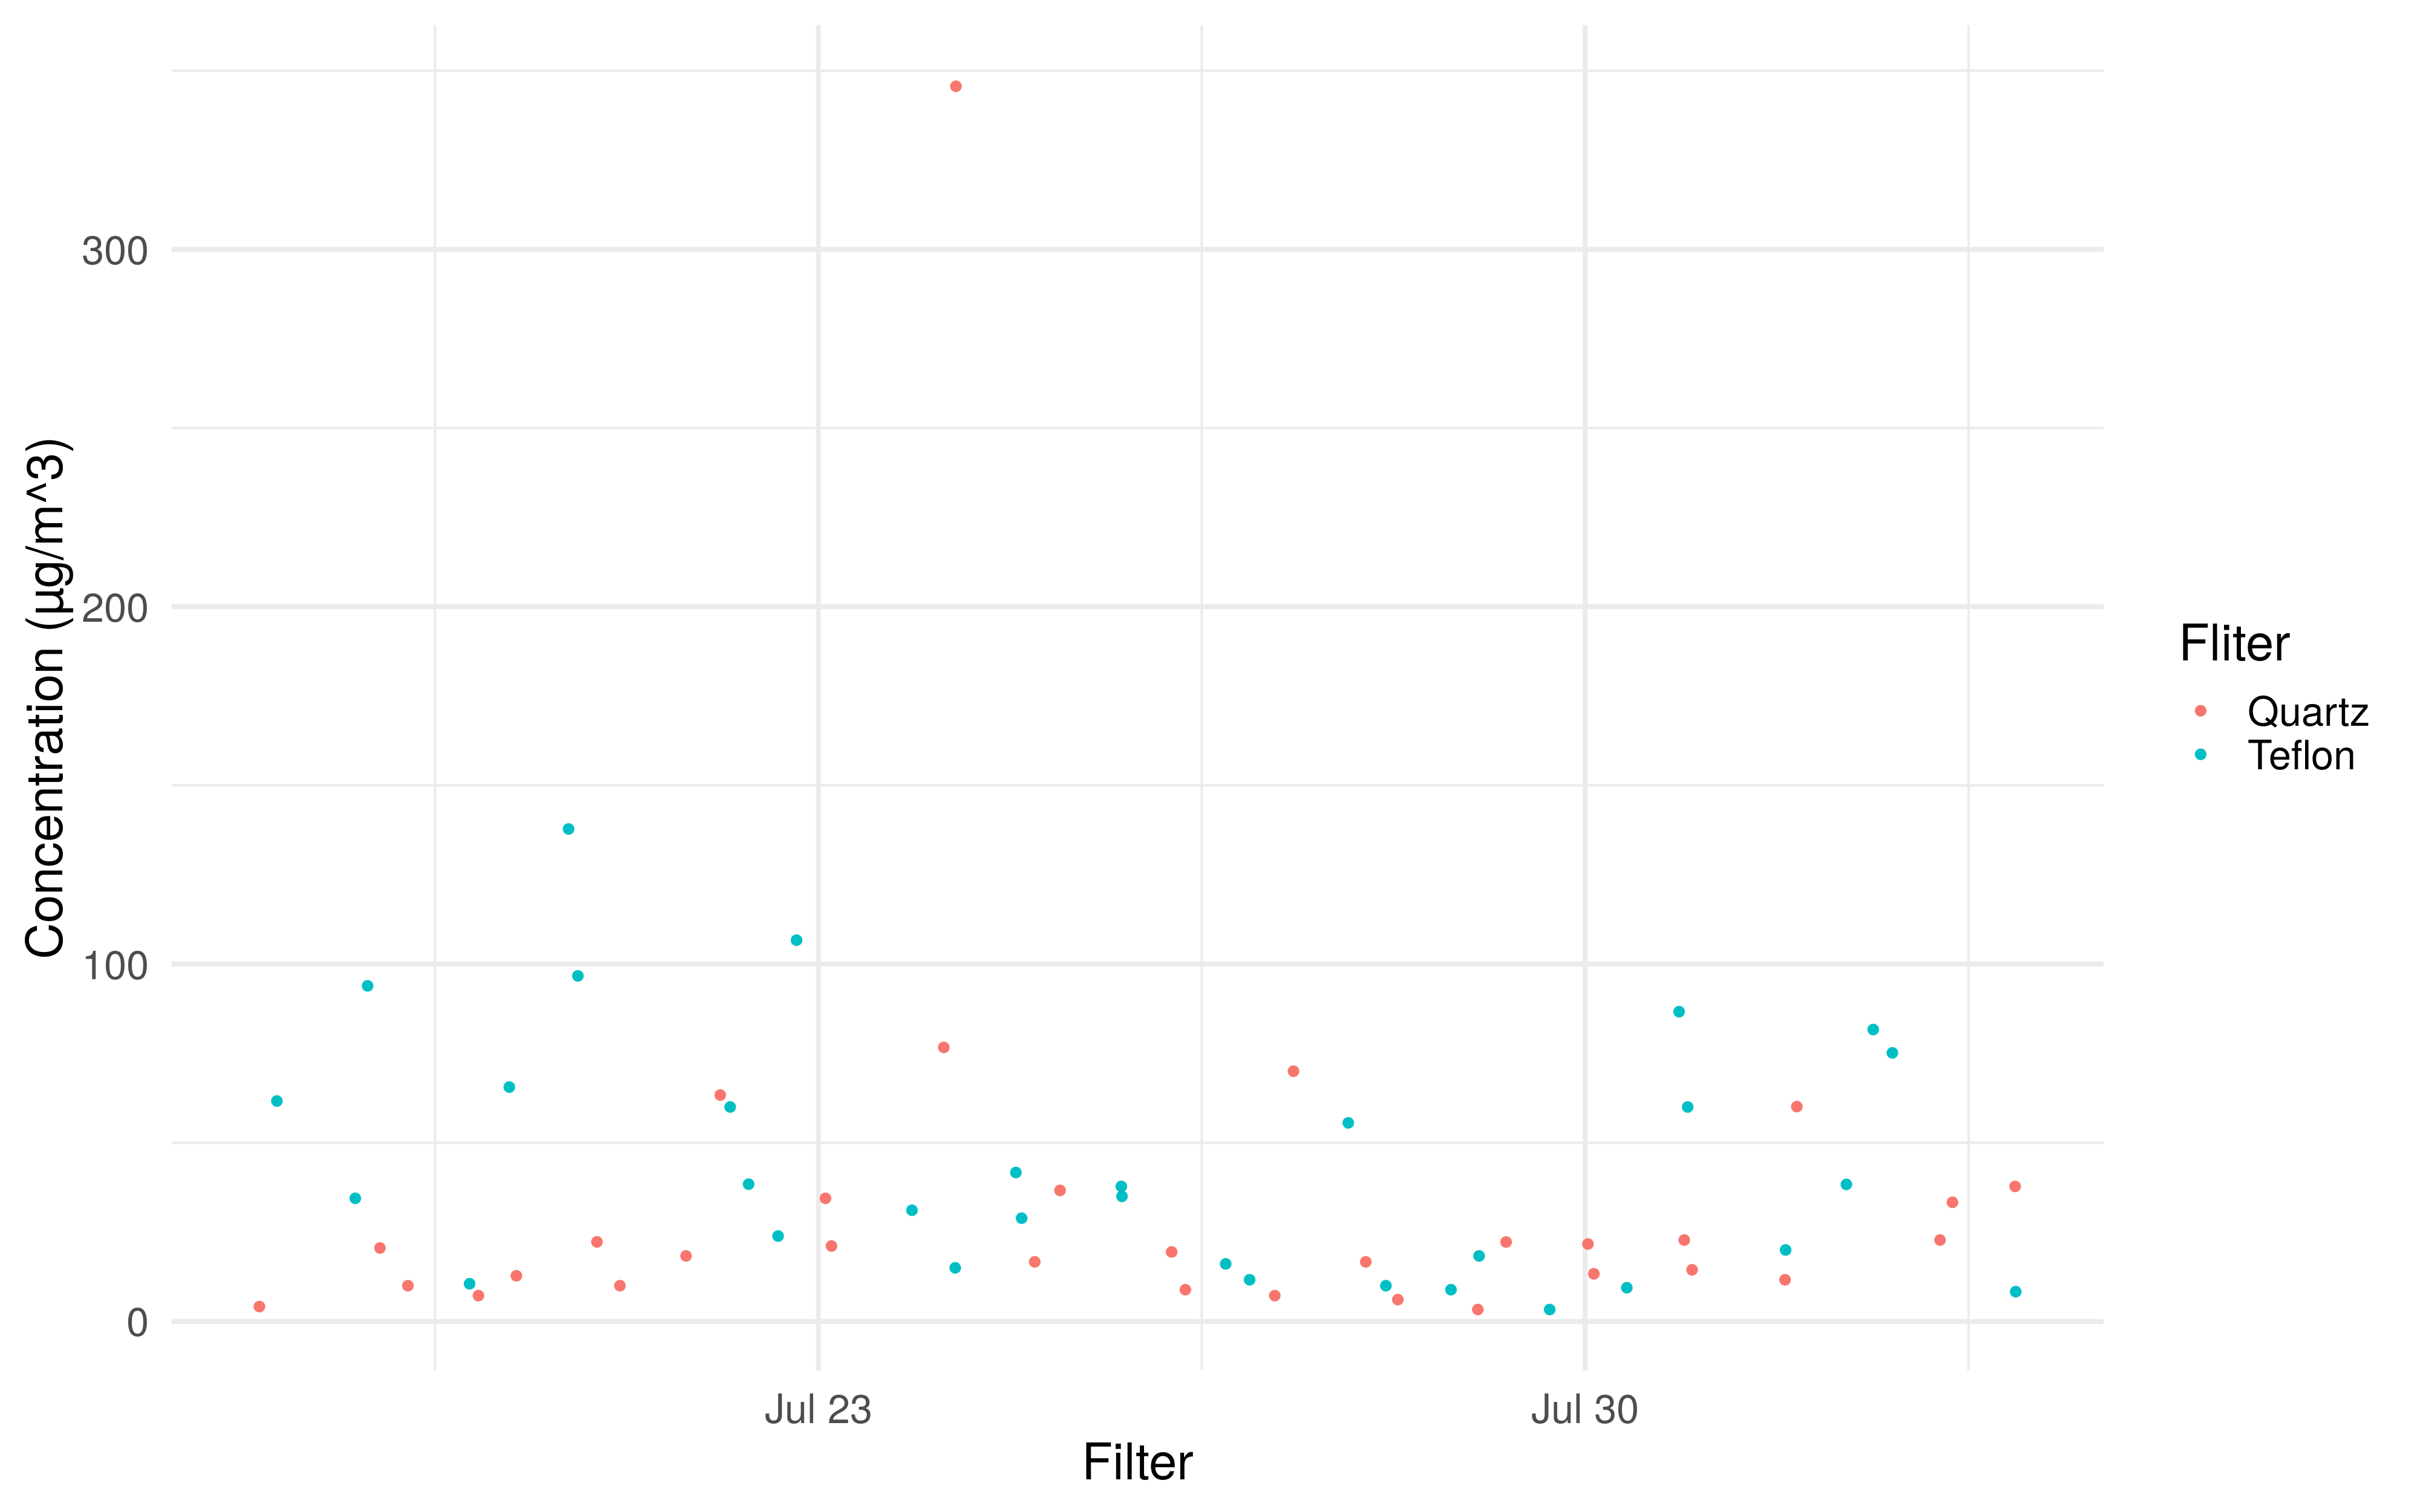
\includegraphics[width=\textwidth]{images/pm25_winter_jitter.png}
    \caption{Caption}
    \label{fig:pm2.5_winter_jitter}
\end{figure}

\begin{figure}[!htb]
    \centering
    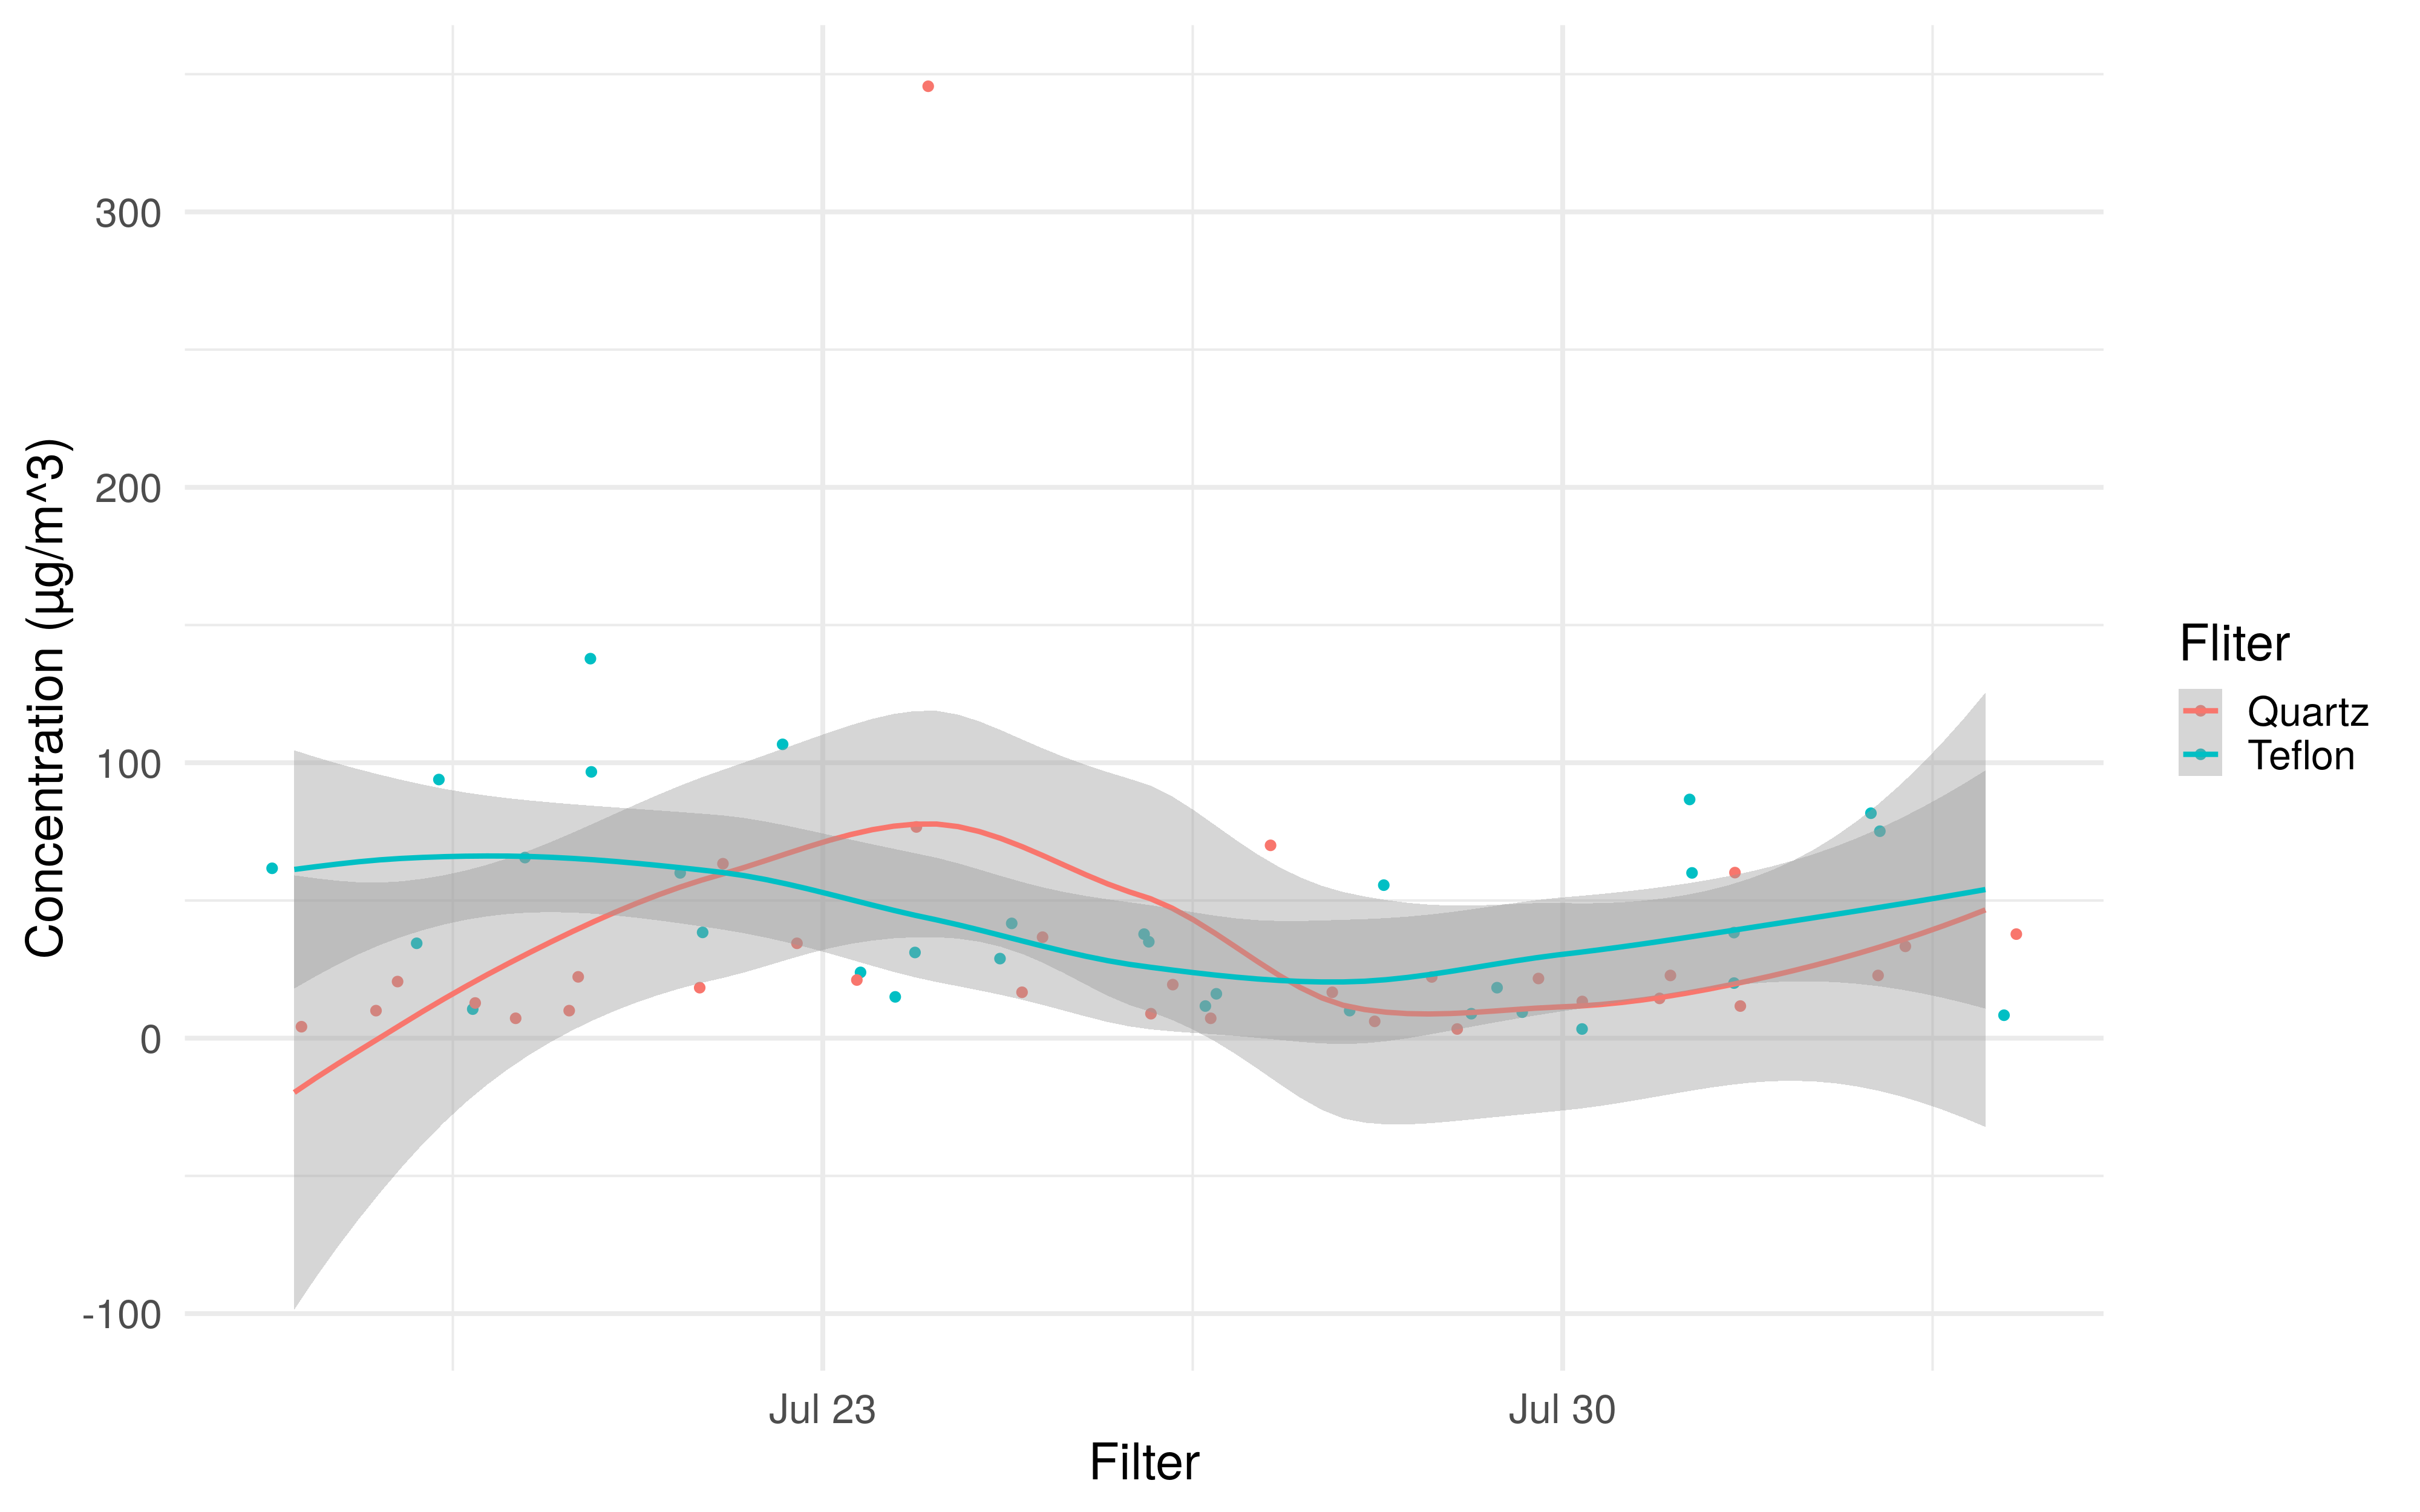
\includegraphics[width=\textwidth]{images/pm25_winter_jittersmooth.png}
    \caption{Caption}
    \label{fig:pm2.5_winter_jitter_smooth}
\end{figure}

\begin{figure}[!htb]
    \centering
    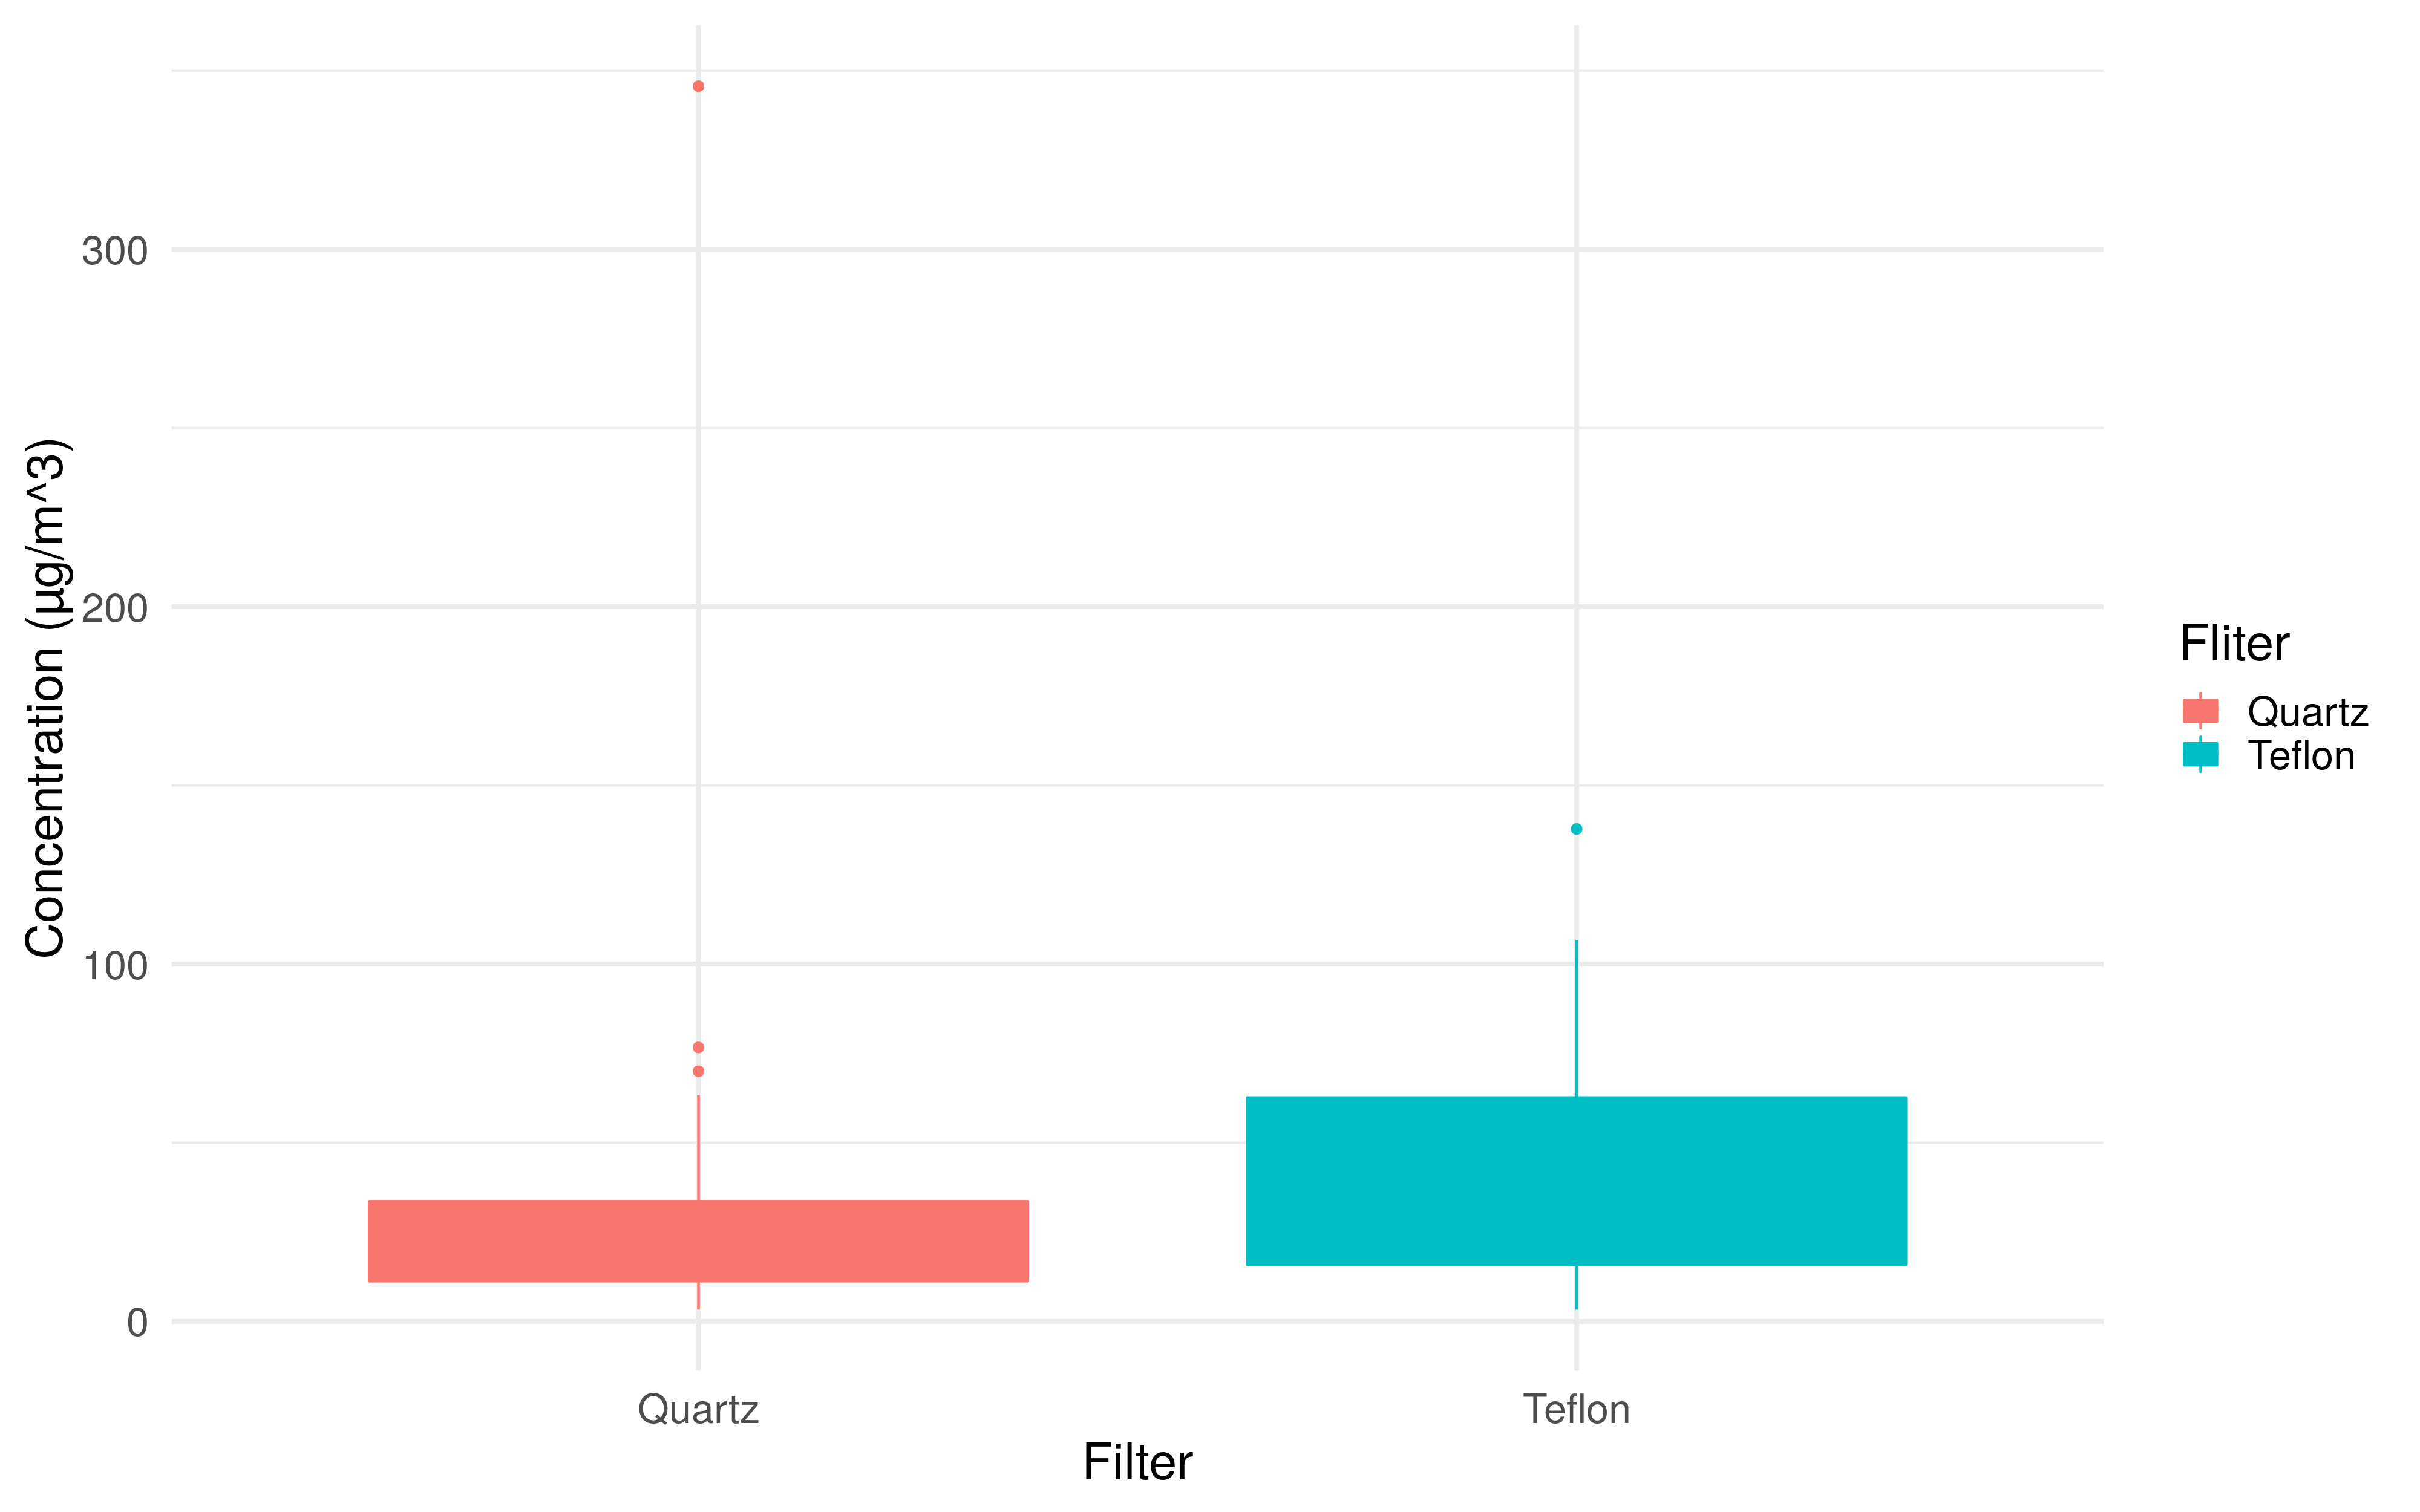
\includegraphics[width=\textwidth]{images/pm25_winter_box_filter.png}
    \caption{Caption}
    \label{fig:pm2.5_winter_box}
\end{figure}

\begin{figure}[!htb]
    \centering
    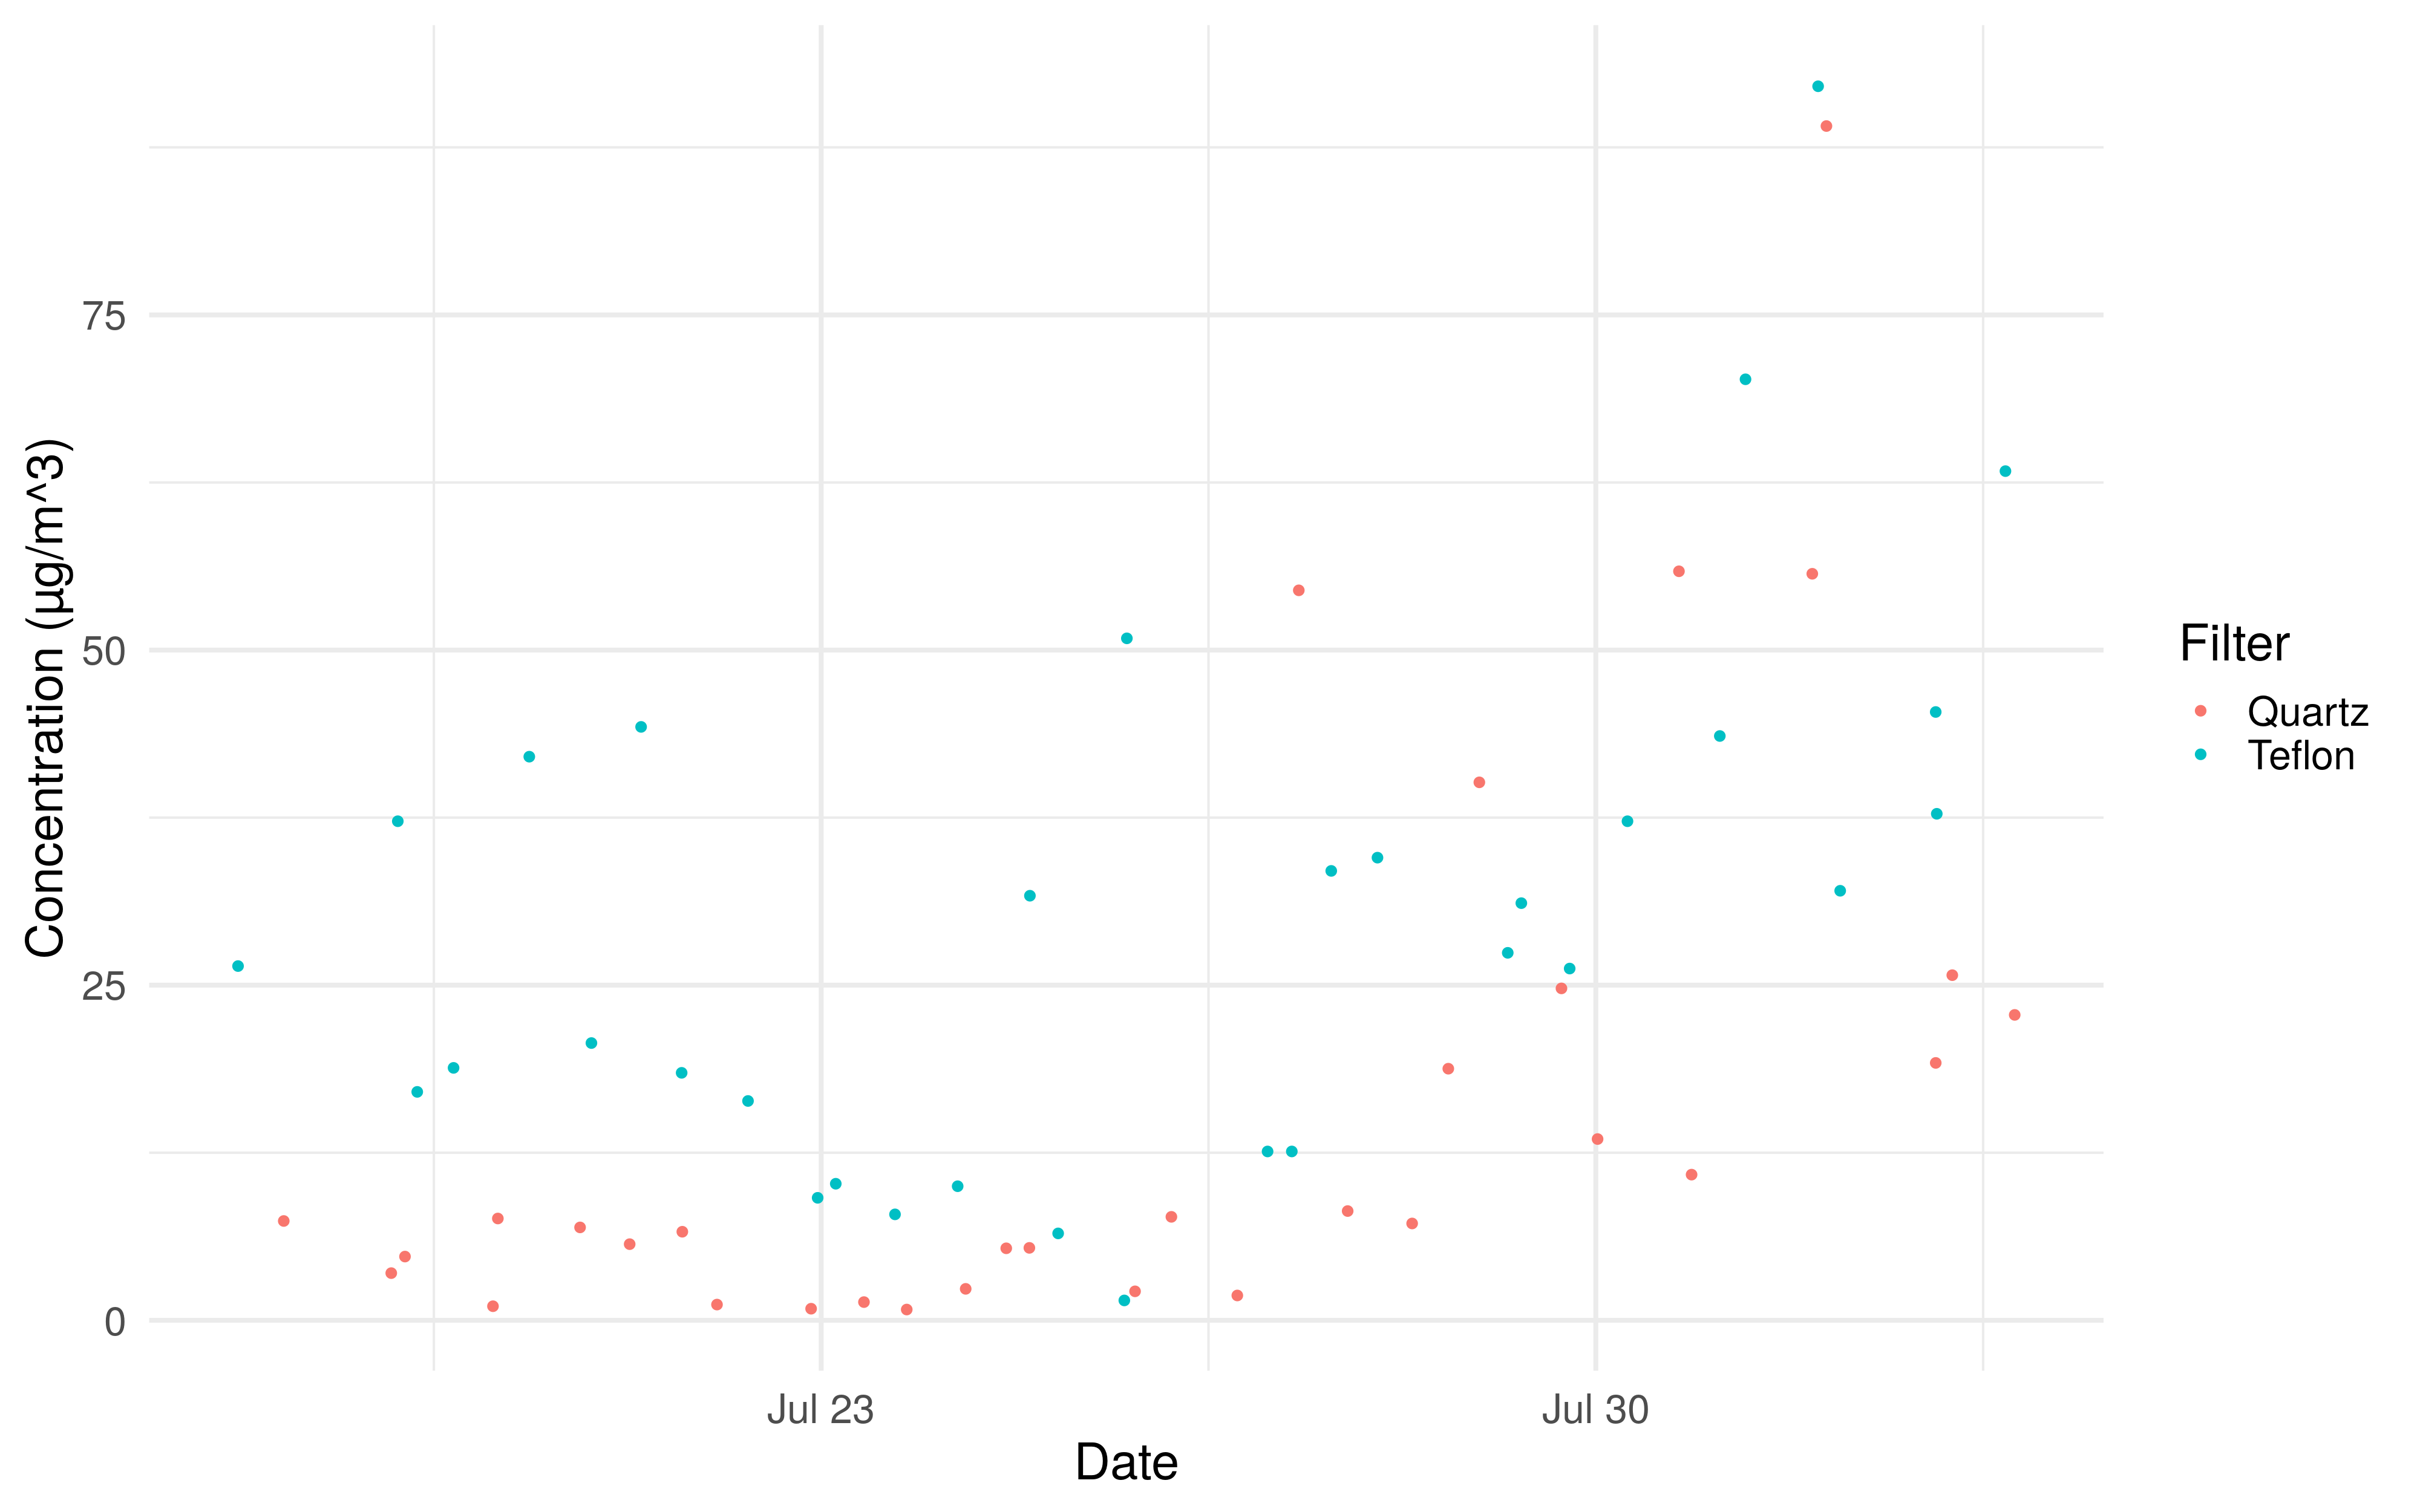
\includegraphics[width=\textwidth]{images/pm10_winter_jitter.png}
    \caption{Caption}
    \label{fig:pm10_winter_jitter}
\end{figure}

\begin{figure}[!htb]
    \centering
    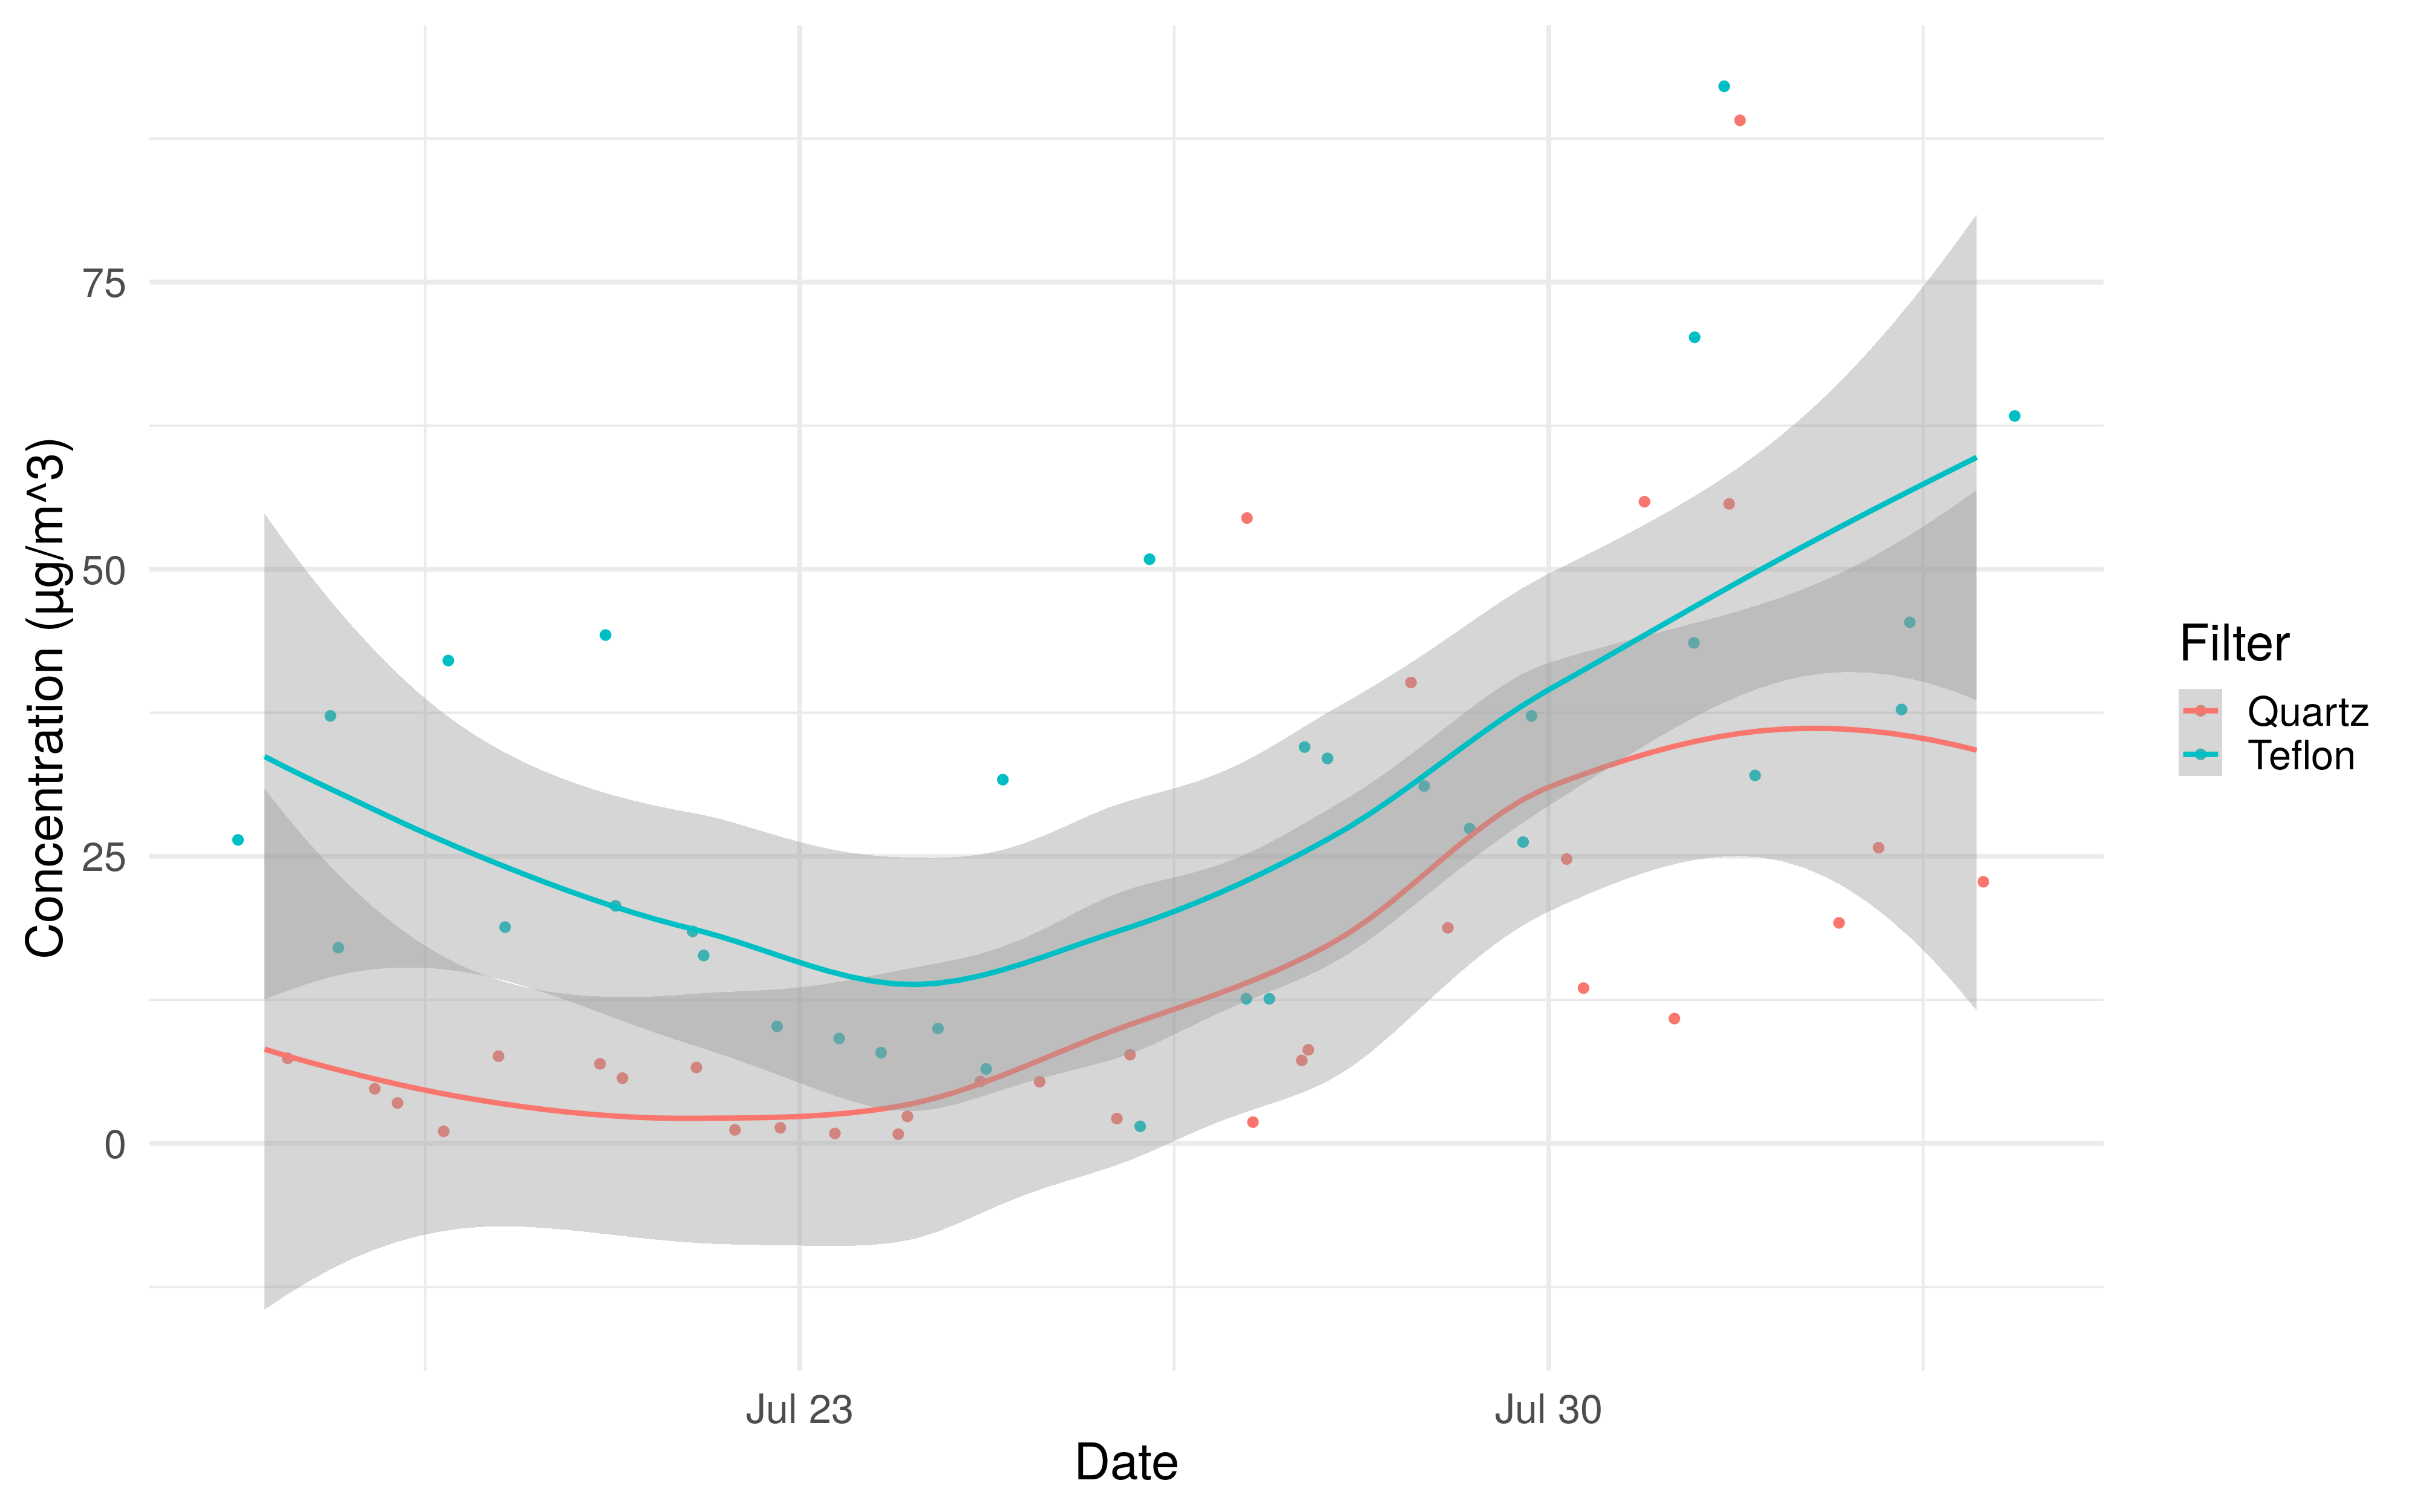
\includegraphics[width=\textwidth]{images/pm10_winter_jittersmooth.png}
    \caption{Caption}
    \label{fig:pm10_winter_jitter_smooth}
\end{figure}

\begin{figure}[!htb]
    \centering
    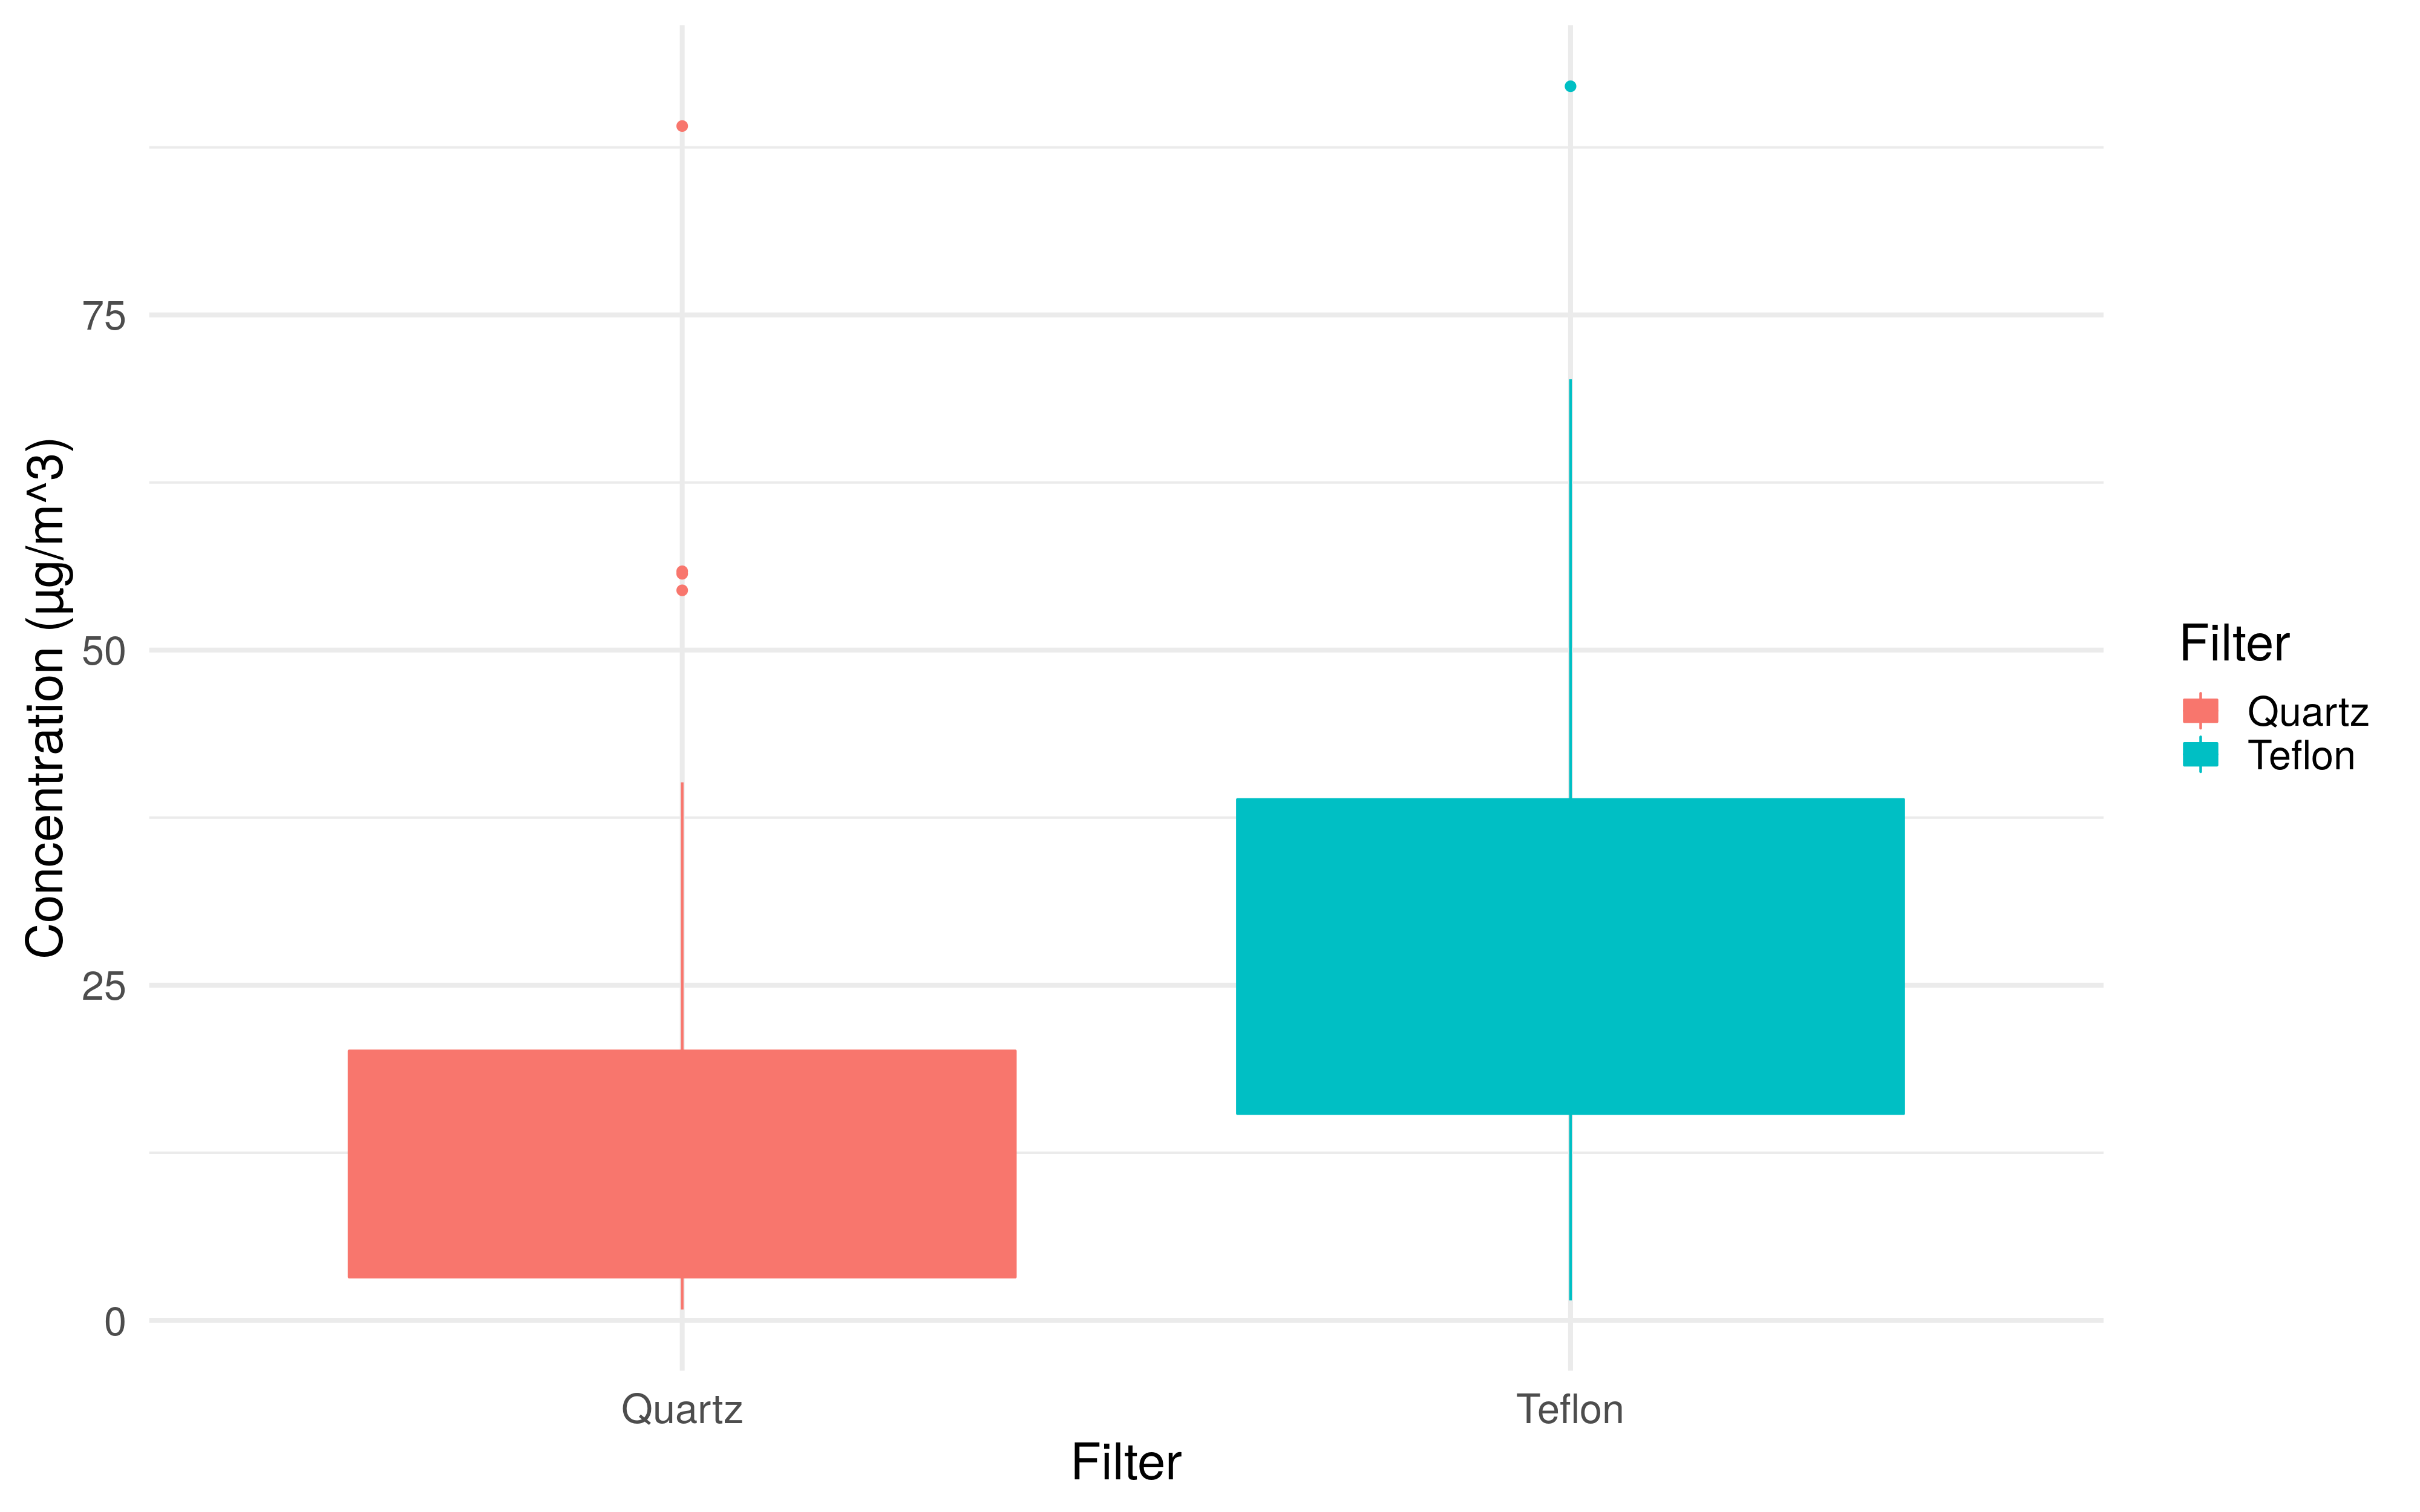
\includegraphics[width=\textwidth]{images/pm10_winter_box_filter.png}
    \caption{Caption}
    \label{fig:pm10_winter_box}
\end{figure}

%%%%%%%%%%%%%%%%%%%%%%%%%%%%%%%%%%%%%%%%%%%%%%%%%%%%%%%%%%%%%%%%

\begin{figure}[!htb]
    \centering
    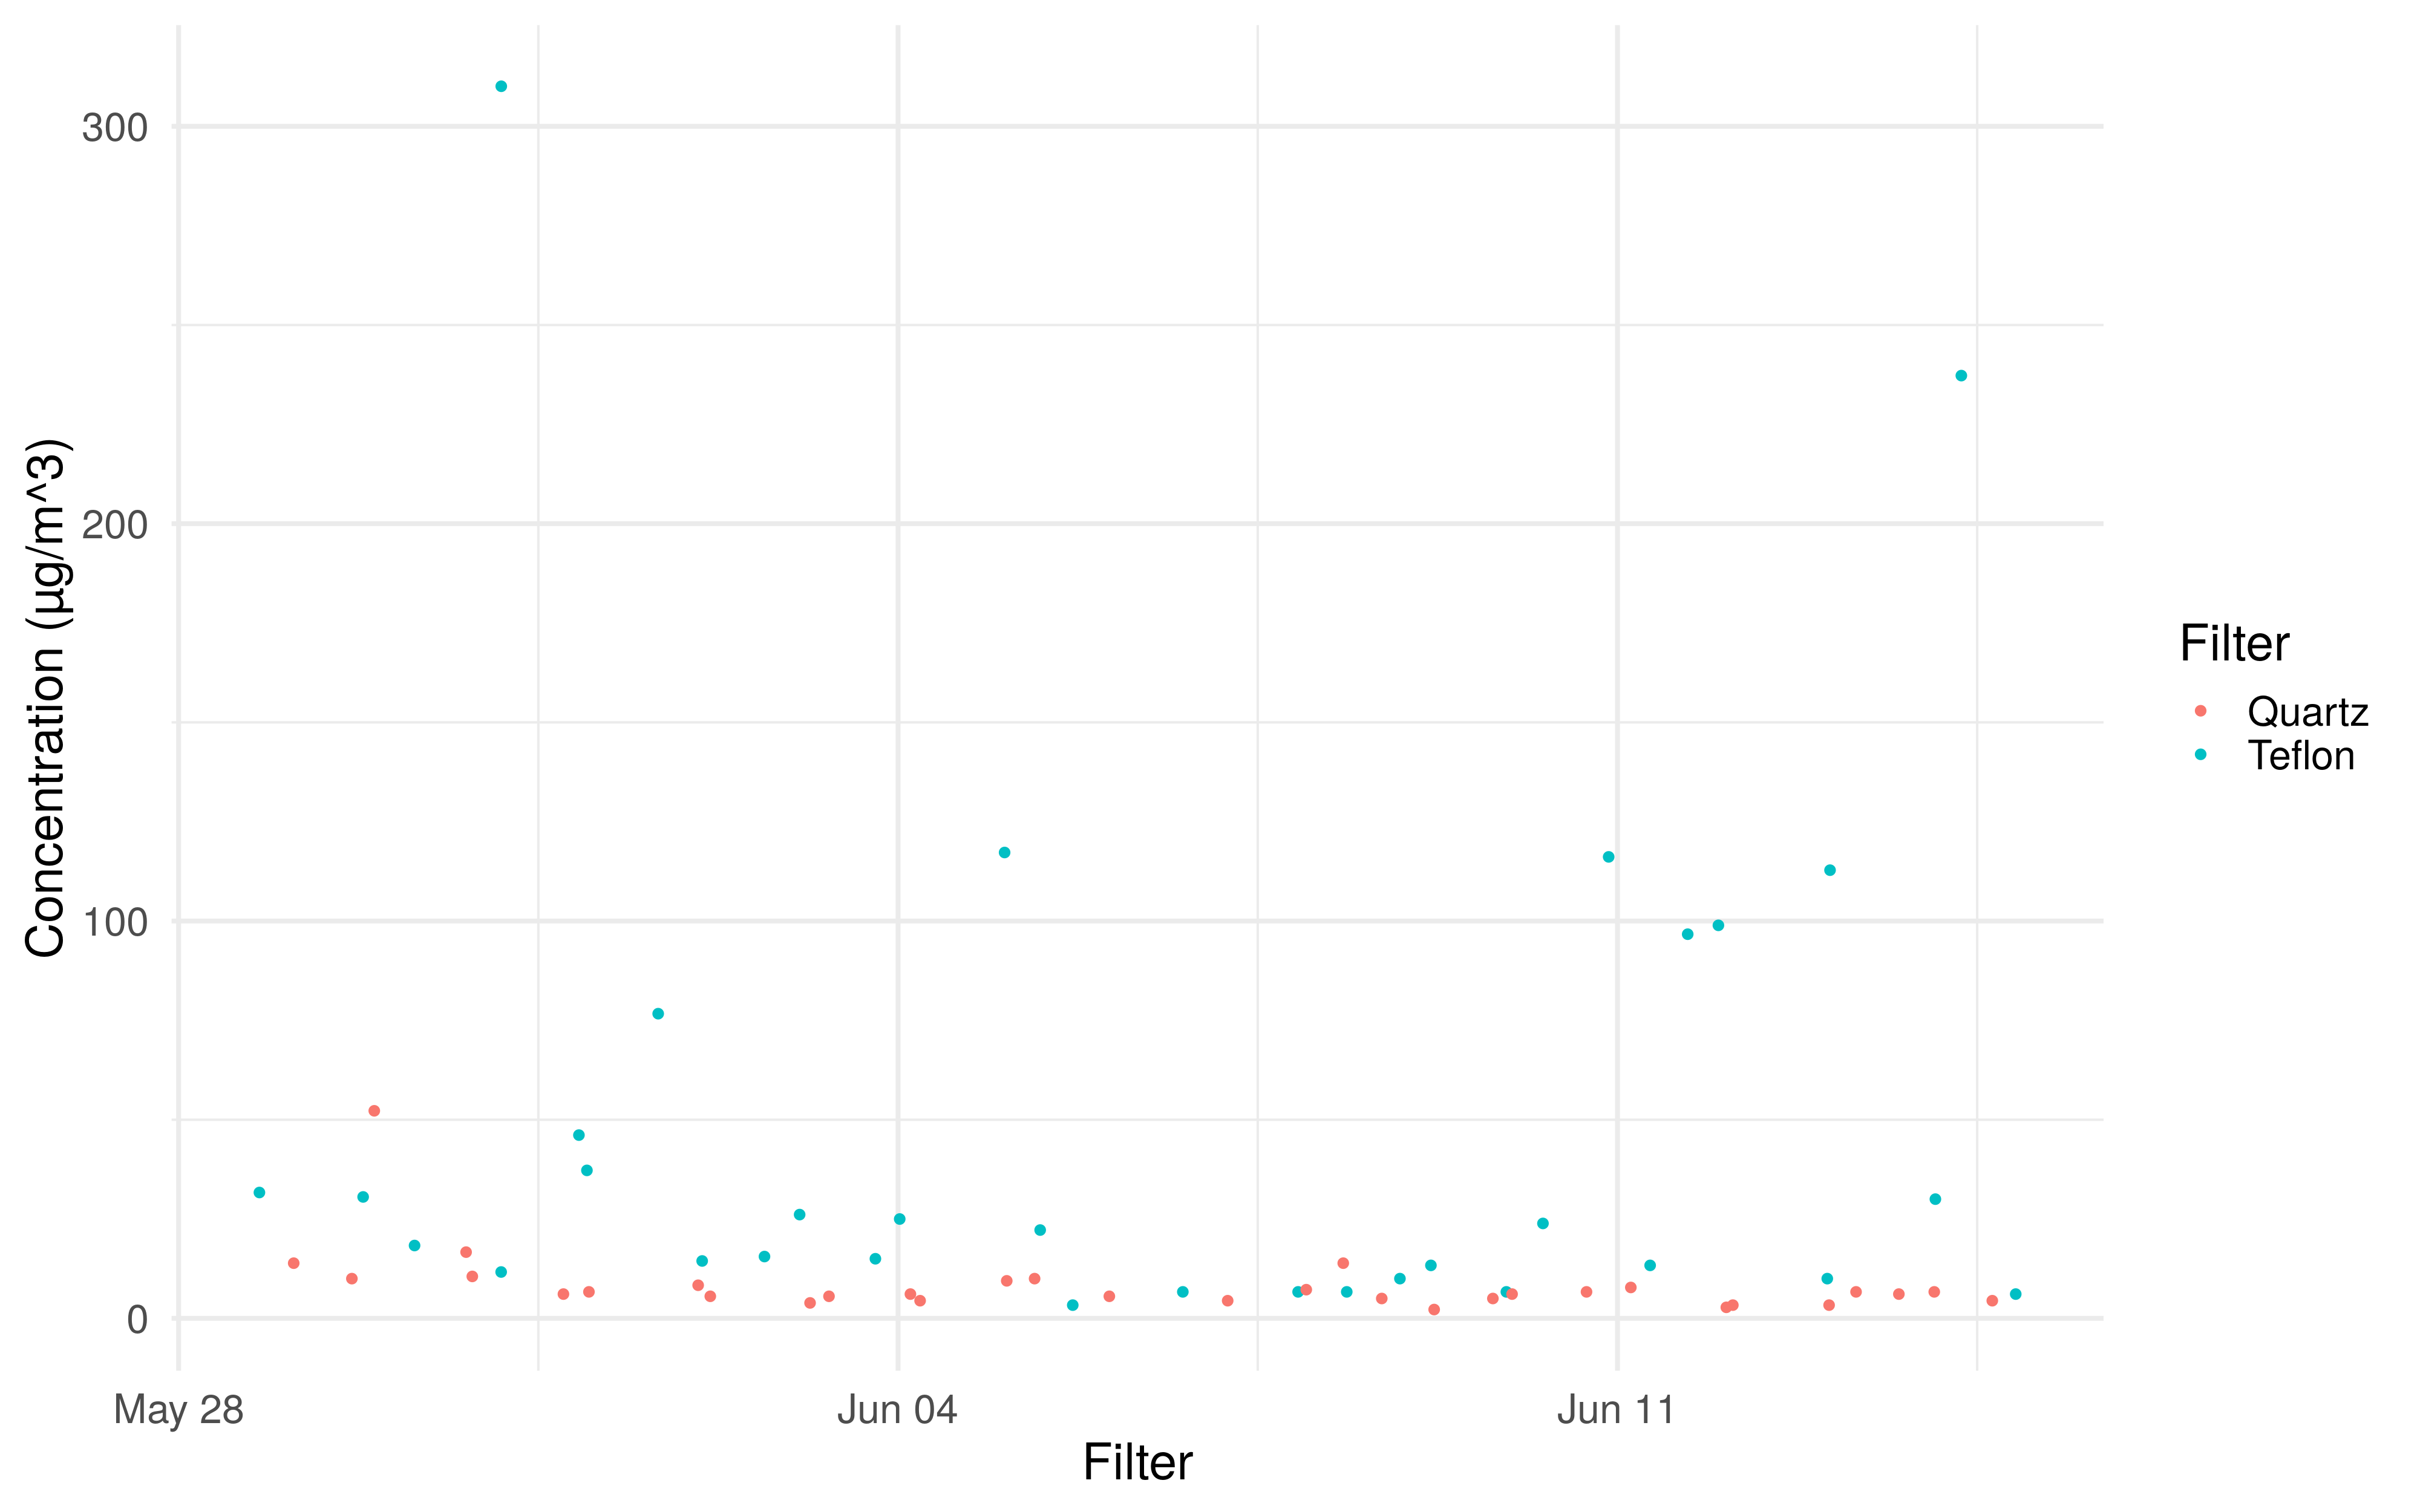
\includegraphics[width=\textwidth]{images/pm25_autumn_jitter.png}
    \caption{Caption}
    \label{fig:pm2.5_autumn_jitter}
\end{figure}

\begin{figure}[!htb]
    \centering
    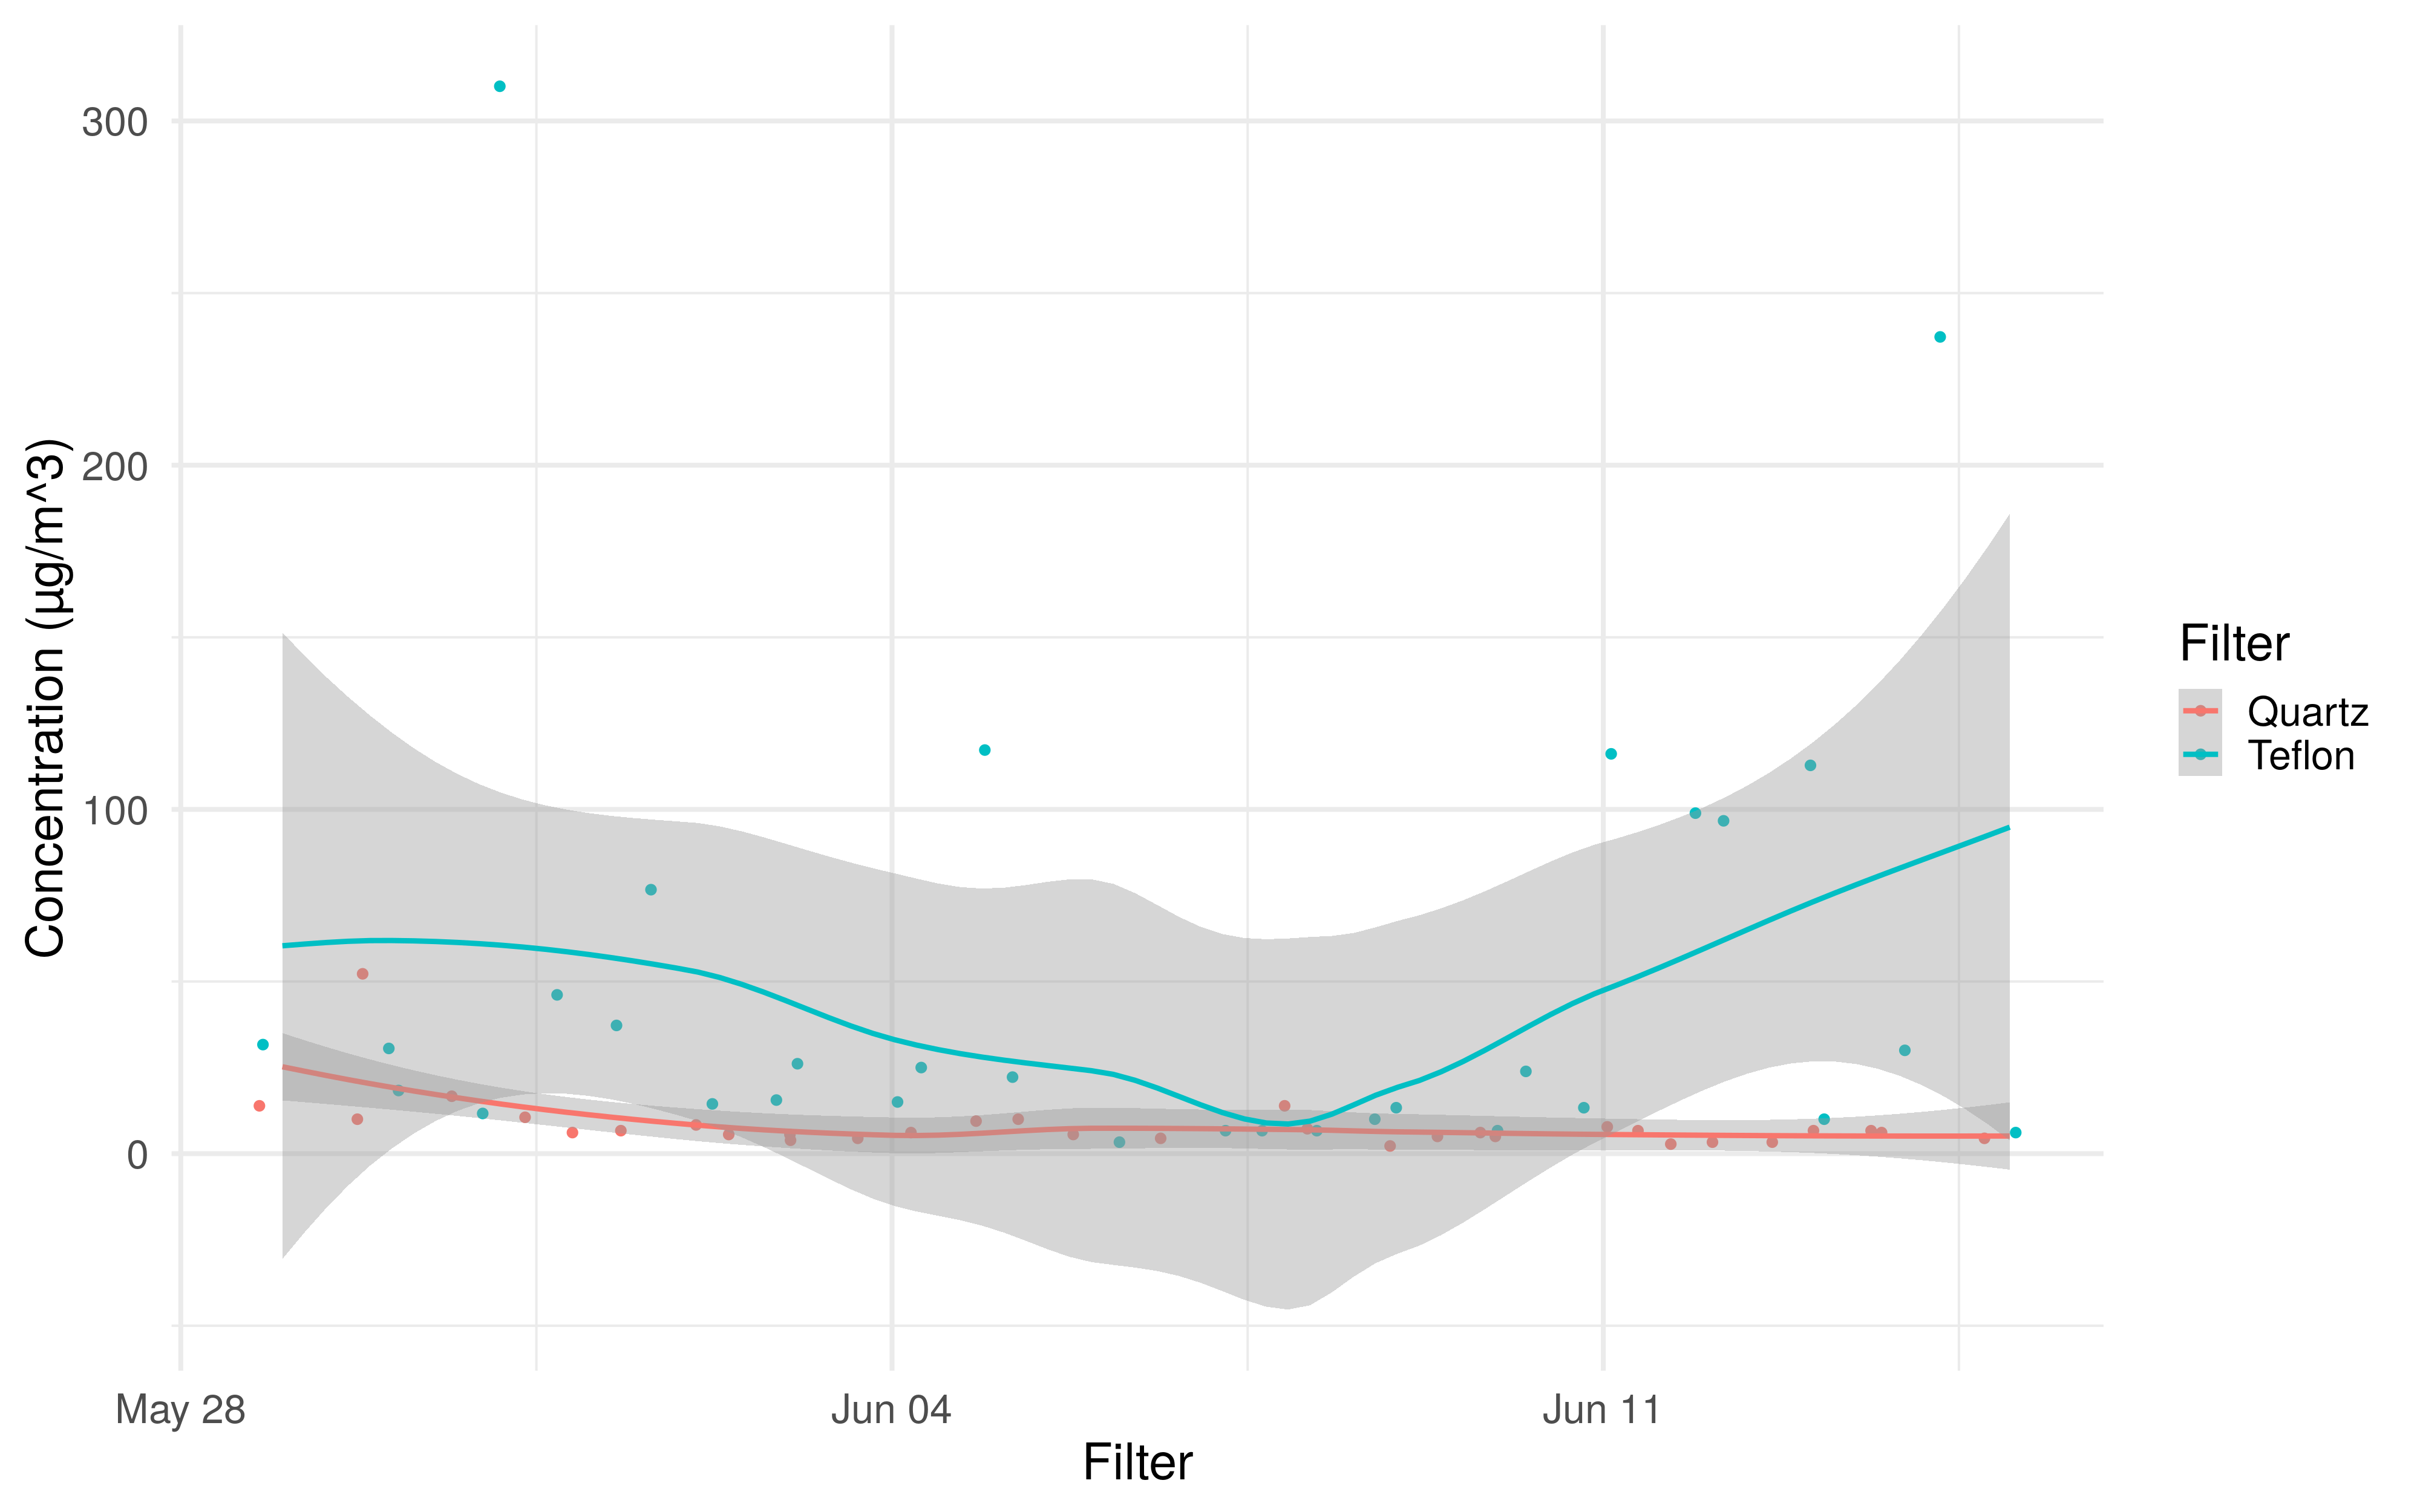
\includegraphics[width=\textwidth]{images/pm25_autumn_jittersmooth.png}
    \caption{Caption}
    \label{fig:pm2.5_autumn_jitter_smooth}
\end{figure}

\begin{figure}[!htb]
    \centering
    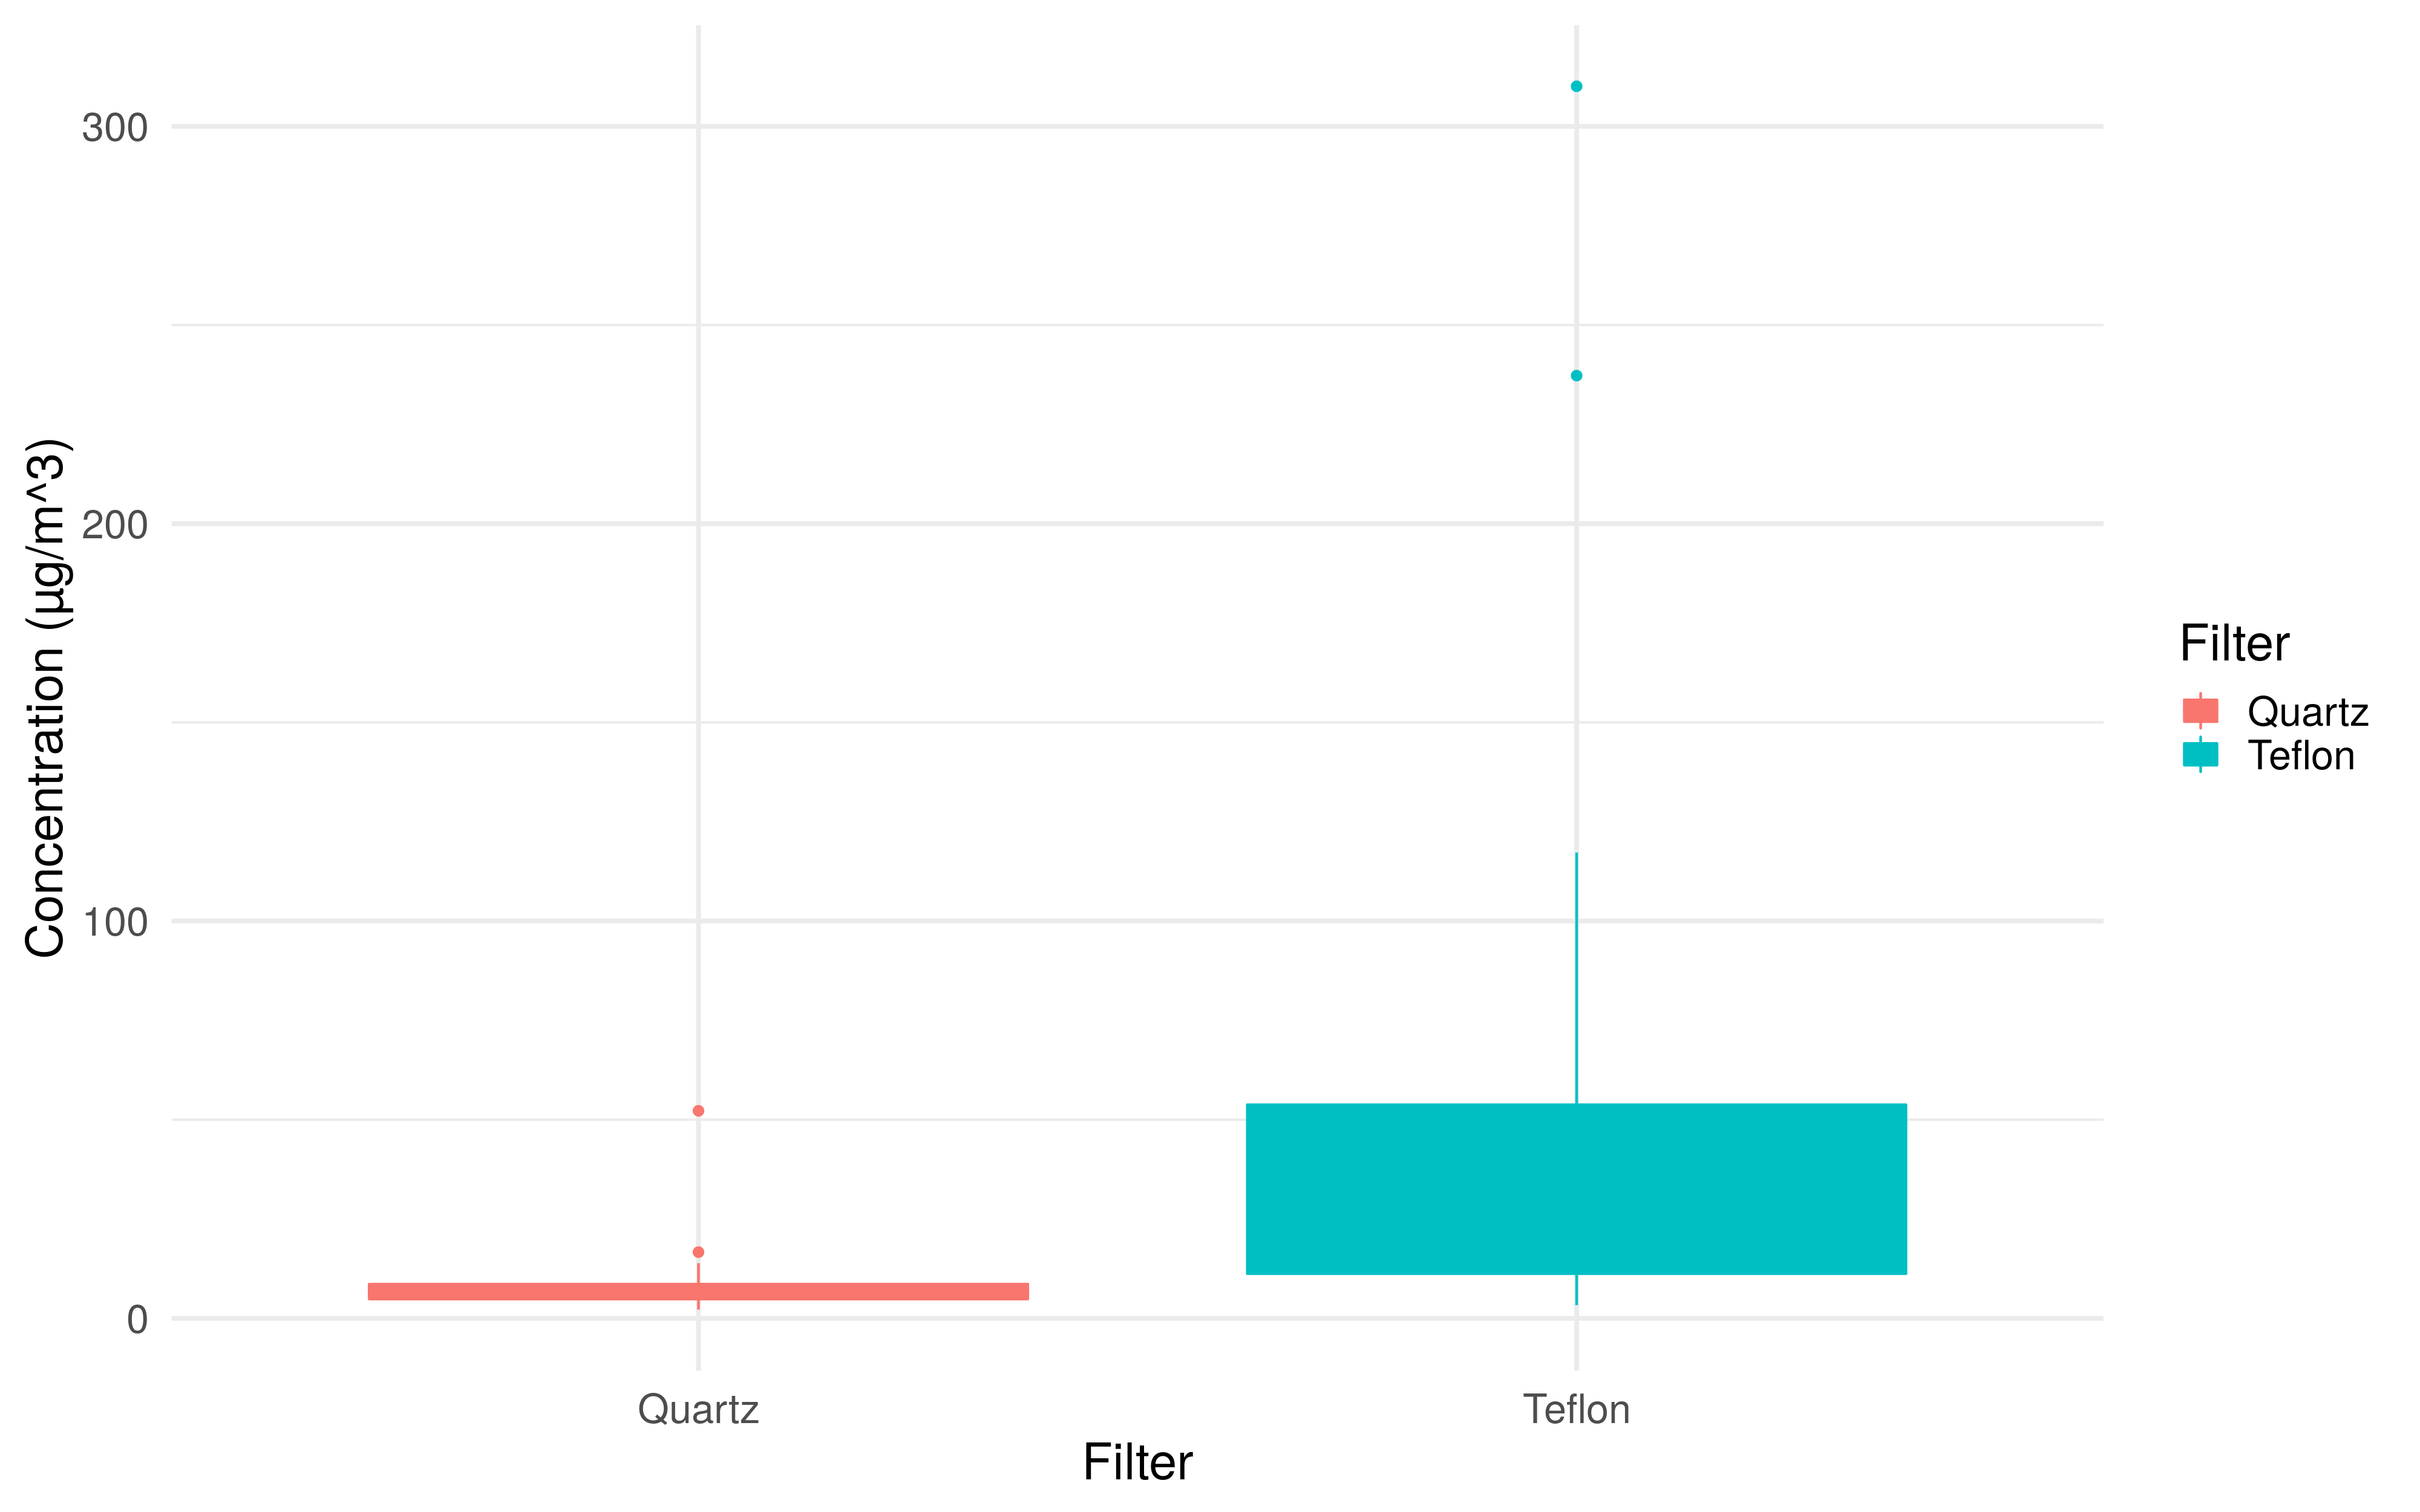
\includegraphics[width=\textwidth]{images/pm25_autumn_box.png}
    \caption{Caption}
    \label{fig:pm2.5_autumn_box}
\end{figure}

\begin{figure}[!htb]
    \centering
    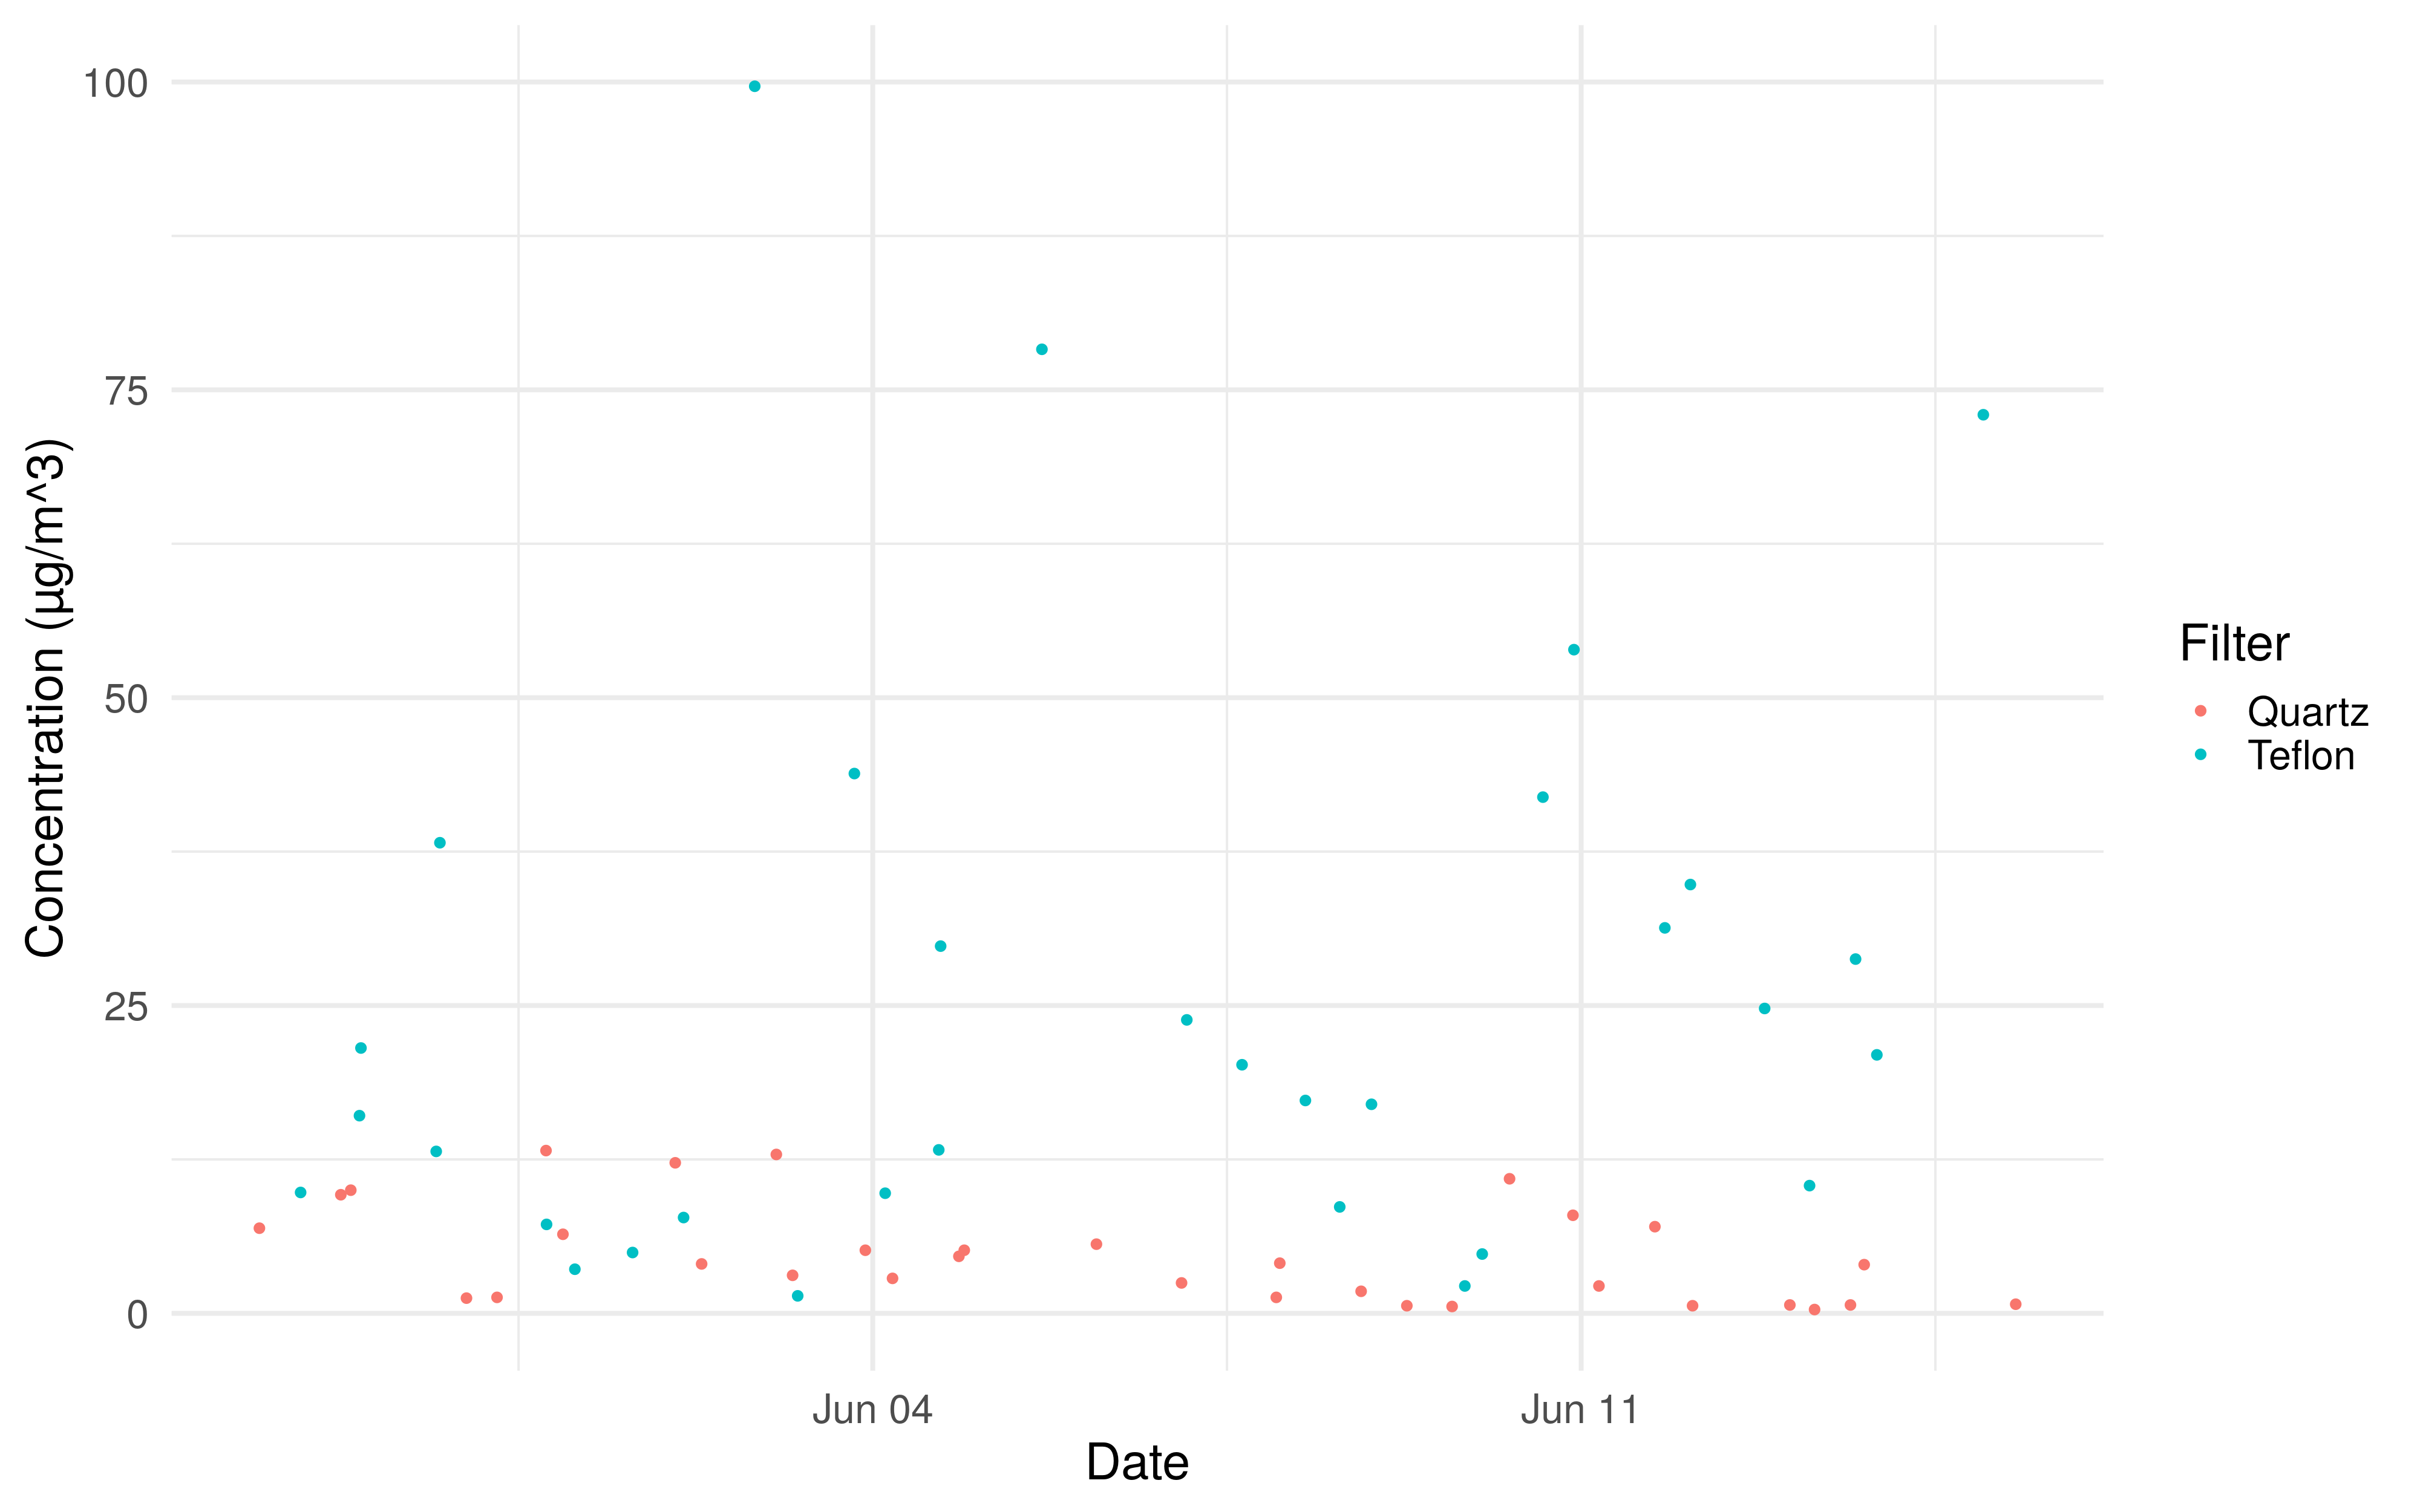
\includegraphics[width=\textwidth]{images/pm10_autumn_jitter.png}
    \caption{Caption}
    \label{fig:pm10_autumn_jitter}
\end{figure}

\begin{figure}[!htb]
    \centering
    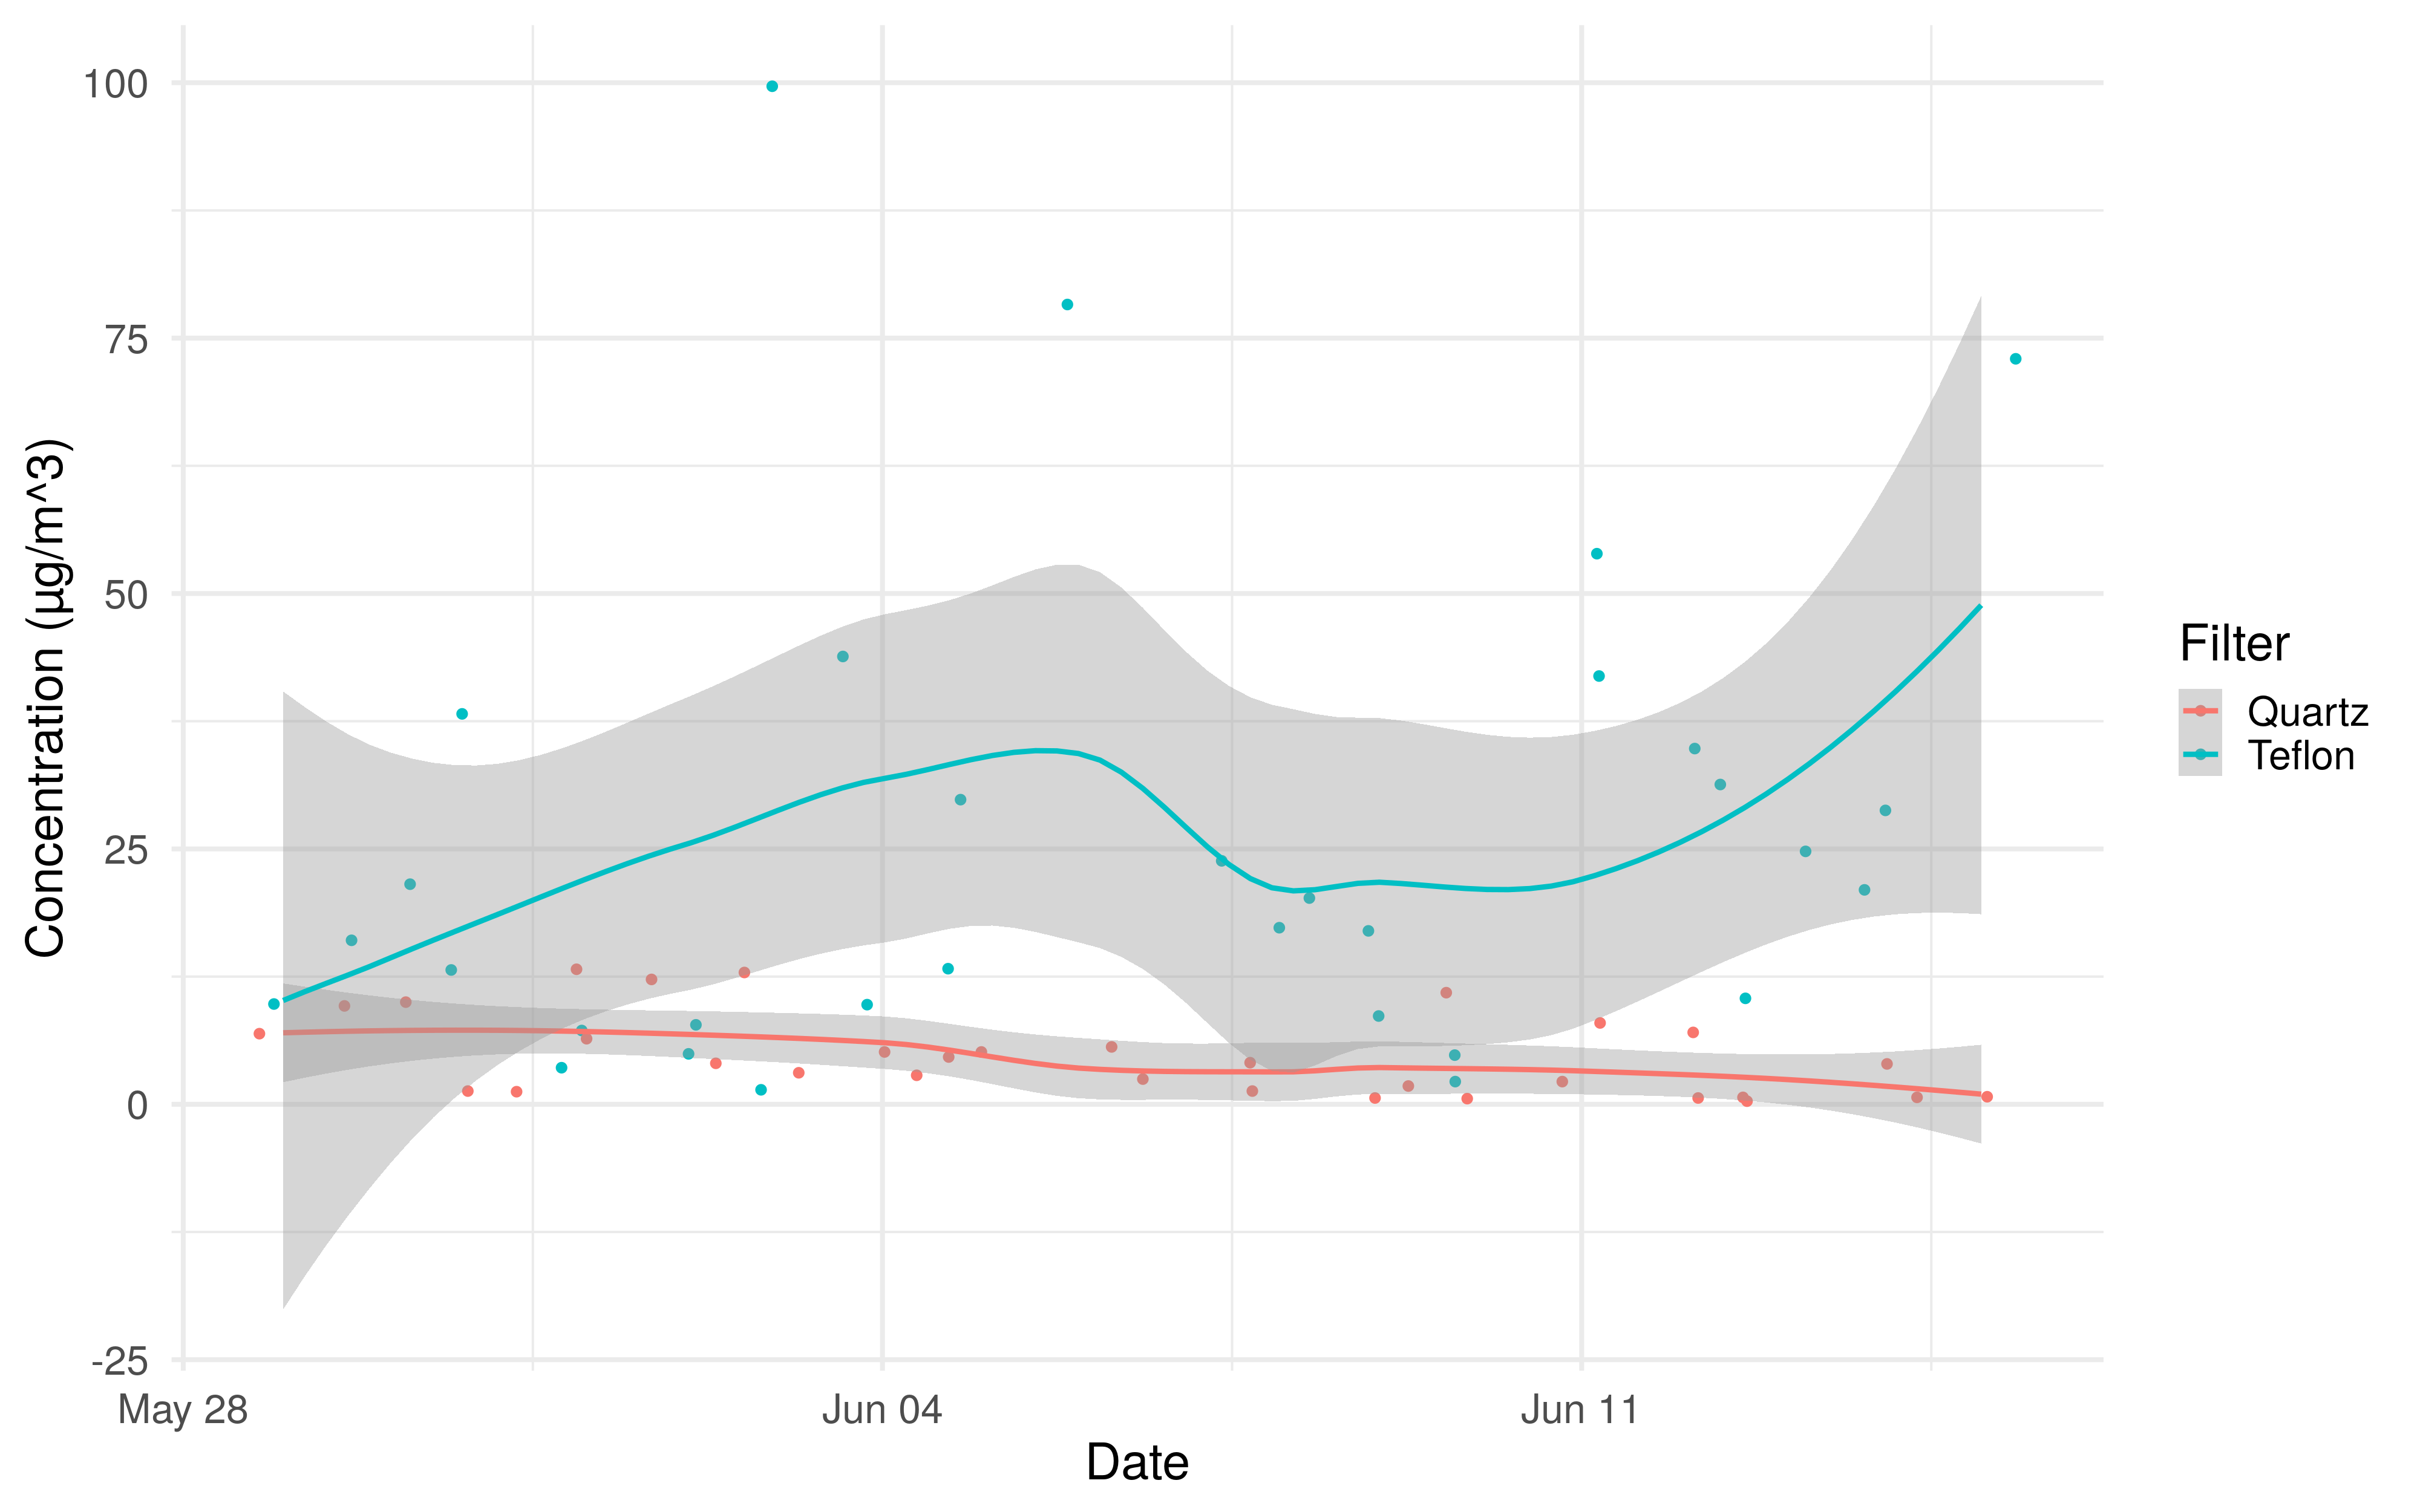
\includegraphics[width=\textwidth]{images/pm10_autumn_jittersmooth.png}
    \caption{Caption}
    \label{fig:pm10_autumn_jitter_smooth}
\end{figure}

\begin{figure}[!htb]
    \centering
    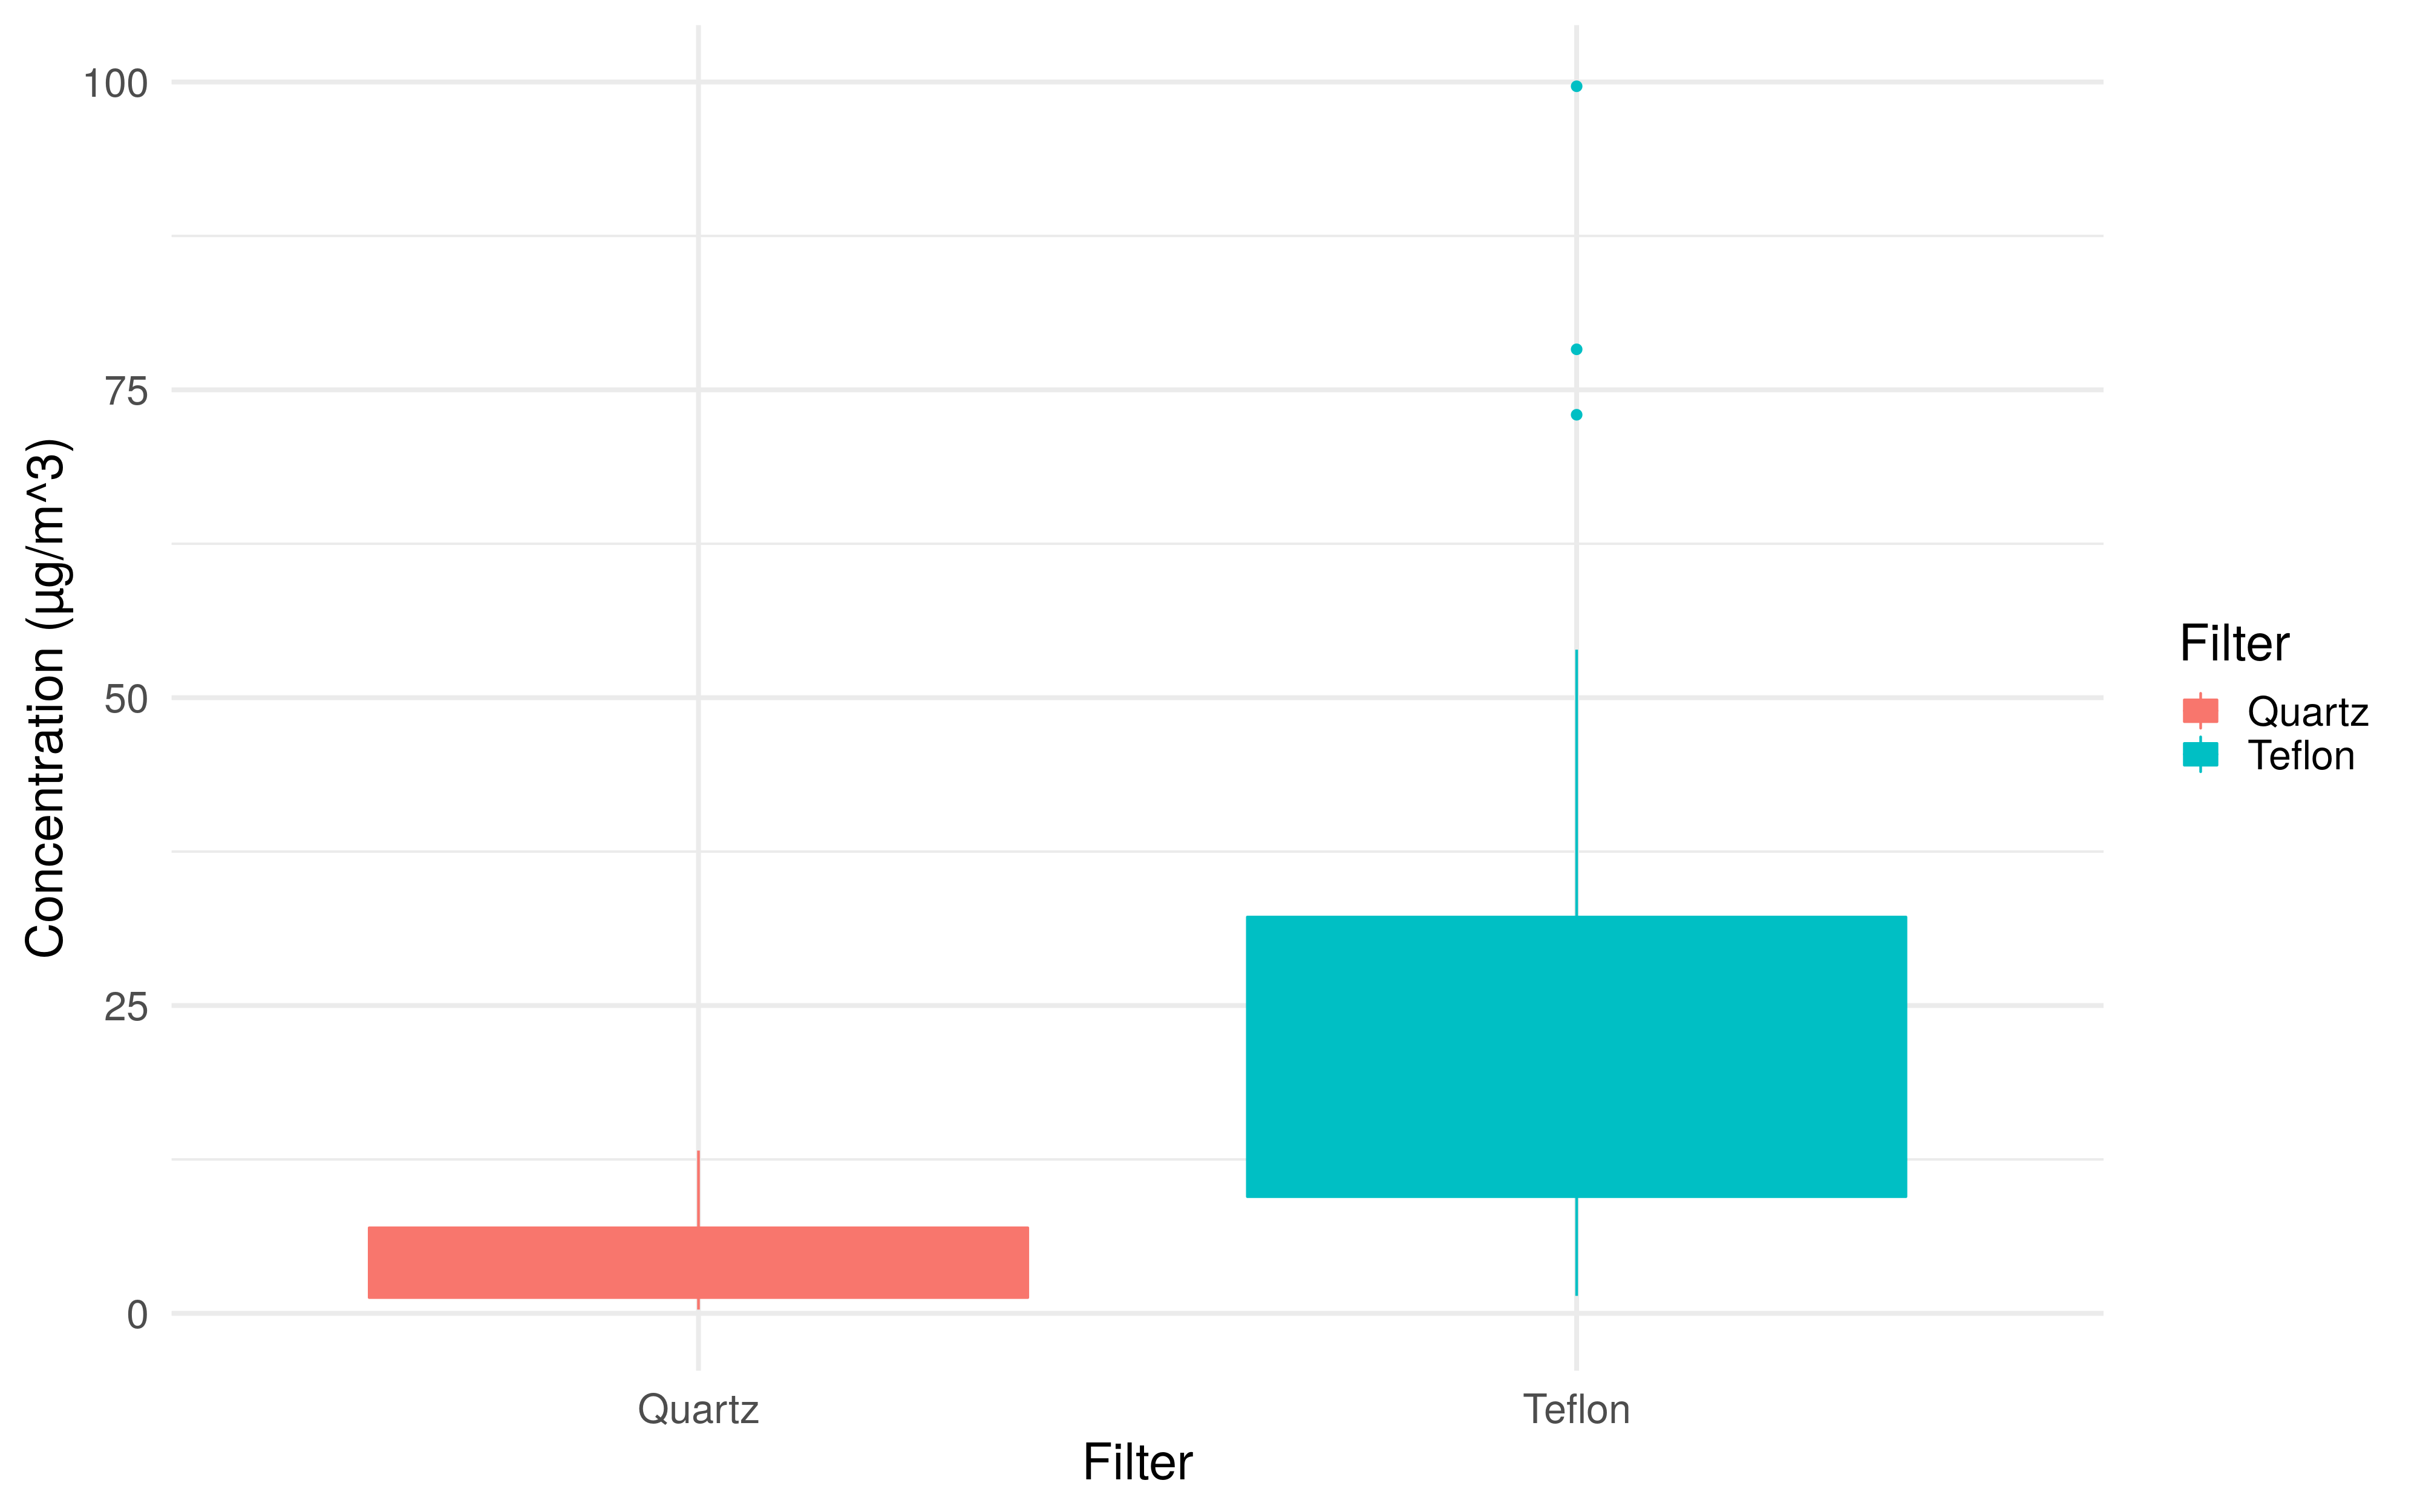
\includegraphics[width=\textwidth]{images/pm10_autumn_box_filter.png}
    \caption{Caption}
    \label{fig:pm10_autumn_box}
\end{figure}

What have we been doing so far

%%%%%%%%%%%%%%%%%%%%%%%%%%%%%%%%%%%%%%%%%%%%%%%%%%%%%%%%%%%%%

\chapter{Source apportionment campaigns}

Describe the campaigns and list data collected

%%%%%%%%%%%%%%%%%%%%%%%%%%%%%%%%%%%%%%%%%%%%%%%%%%%%%%%%%%%%%

\chapter{Conclusions}

What is the next step of the project 

\section{Next steps}

\section{Potential problems}

%%%%%%%%%%%%%%%%%%%%%%%%%%%%%%%%%%%%%%%%%%%%%%%%%%%%%%%%%%%%%

\begin{spacing}{0.3}
\linespread{0.8} \normalsize
\bibliography{library}
\end{spacing}

\end{document}